\documentclass[12pt,a4paper,normalheadings,titlepage]{scrreprt}

\usepackage{../common/evman}
\usepackage{graphicx}

\pagestyle{headings}

\def\title{RT-Druid reference manual}
\def\subtitle{A tool for the design of embedded real-time systems}
\include{dynamic_version}


%\usepackage[T1]{fontenc}
%\usepackage[latin1]{inputenc}
%\setcounter{secnumdepth}{3}
%\setcounter{tocdepth}{3}
%\usepackage{makeidx}
%\makeindex
%\usepackage{babel}

\begin{document}

\maketitle

\tableofcontents{}


\chapter{Introduction}
\label{cha:intro}

This document provides the user with a basic understanding of the
architecture, the features and the operations of \rtd\ and the
associated \ee\ Kernel.

\rtd\ is now fully integrated with the open source Eclipse framework,
as is distributed as a set of plugins that can be installed on top of
various Eclipse versions.

This document covers the description of two main components of \rtd,
which are the code generator plugins for OSEK/VDX systems and the
schedulability analysis plugins.

The Code generator plugins consists of a {\em core} component,
required for all operations, and a number of plugins providing time
verification and automatic generation of the implementation of
real-time embedded software.

The Schedulability analysis plugins provides schedulability analysis
support, allowing the user to model the application architecture using
the \rtd\ metamodel. Once modeled, the system can be analyzed using
the schedulability tests, providing in this way useful information
such as task response times, and sensitivity analysis.


\section{Software design with \rtd{}}

The architecture of \rtd\ is shown in Figure
\ref{fig:rtdruid-plugin-architecture}. Model information (i.e. for
both the functional and the architecture-level components) is stored
in an internal repository and it is made available by means of an open
format based on XML.

The toolset architecture is based on a kernel, or Core module, providing
management of internal data structure and basic services for GUI and
additional plugin modules.

Plugins exploit kernel services in order to provide support to the
design stages in a completely independent way. Here is a list of the
plugins currently available:

\begin{itemize}
\item \rtd\ Modeler;
\item \rtd\ Schedulability Analyzer;
\item \rtd\ Code generator from OIL/AUTOSAR XML;
\end{itemize}
%
\begin{figure}
\begin{center}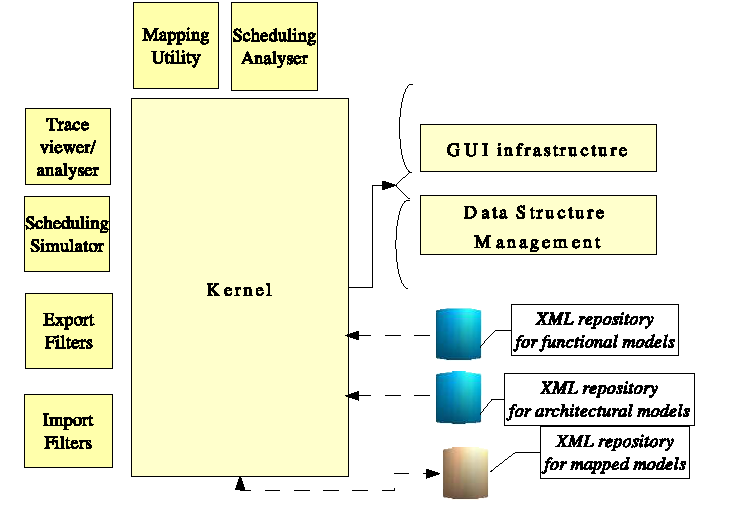
\includegraphics[%
  scale=0.7,bb=0 0 736 529]{images/rtd_plugin_arch.png}\end{center}
\caption{\label{fig:rtdruid-plugin-architecture}The plug-in architecture of \rtd.}
\end{figure}



\section{The open architecture of the \rtd\ tool}

%
\rtd\ allows saving all system information in an open XML
format. Information about the system model, configuration information
and the result of operations performed by plug-in tools, such as
schedulability analysis, tracing or debugging info, can easily be made
available to external or third party tools. Similarly, OIL files can
be imported from or exported to third party products.


\section{\rtd\ integration with Eclipse}

\rtd\ is entirely written in Java. It is based on well-known
development frameworks such as Eclipse, the framework originally
propoted by IBM and now released as an open source development
environment \cite{Eclipse}, and on the W3C XML standard. The \rtd\ tool
makes use of several Eclipse plug-ins, including EMF
\cite{Eclipse-EMF}, GEF \cite{Eclipse-GEF} and CDT
\cite{Eclipse-CDT}\footnote{CDT is the Eclipse component in charge of
C/C++ project management.}.

The integration of \rtd\ with the Eclipse framework easily allows any
user to perform the operations of editing, compiling, debugging and
running the software. The required commands and action sequences are
those common to all Eclipse projects, including CDT.


\section{Content of this document}

The document is divided in two parts. The first one is
dedicated to the code generator plugins, whereas the second one is
dedicated to the schedulability analysis plugins.

The first part about the code generator plugins contains the basic
information for operating with the tool and providing the right
configuration input for the code generation phase. 

In Chapter \ref{cha:overview}, the code generator plugins are
introduced, the code generation process is outlined and the
relationships among the products and the Eclipse development
environment are explained.

Chapter \ref{cha:creating-rtdruid-project} explains the basic steps
that are necessary to start an Rt-Druid project and how to define the
basic configuration info that is required by the tool. A fundamental
part of the configuration tool is contained in the OIL input
file. Syntax and methods for generating the OIL description of the
system are the subject of Chapter \ref{cha:oil-syntax}. The
\ee\ specific extensions to the OIL language that are necessary to
define task placement and other features of multicore systems are
described in Section \ref{sec:oil-multicore}.

The operations that are required for the code generation phase,
together with a detailed description of the input and output data at
each step is the subject of the Chapter \ref{cha:code-generation}.
The kernel configuration and the explanation of the programming model
that needs to be used for \rtd/\ee\ applications are also described in
Chapter \ref{cha:code-generation}.

Finally, the first part of the document concludes with a description
of the \rtd\ standalone version, which is a command-line version of
the code generation plugins, to be used without the Eclipse graphical
interface (see Chapter \ref{cha:Commandline}).

The second part of the document is related to the Schedulability
analysis plugins. The second part starts with Chapter
\ref{cha:schedulability-analysis-introduction}, which gives an
introduction to the purpose of the Schedulability Analysis
plugins. After that, the RT-Druid input file is described in detail
(Chapter \ref{cha:DTD-Input-file}).

Finally, Appendix \ref{cha:Script-File} contains a description of the
ANT scripting support, which enables to run most of the RT-Druid
operations batch. Appendix \ref{cha:oil-definition} contains a
comprehensive OIL implementation description that can be used as a
startup reference.



\part{Code Generation Plugins}
\chapter{An overview of \rtd\ Code Generator and \ee}
\label{cha:overview}

The \rtd\ Code Generator is an open and extensible environment, based
on XML and open standards allowing the generation of configuration
code for the \ee\ real-time kernel. The code configuration may start
from an OSEK OIL or an AUTOSAR XML definition, to create the
configuration code for applications running in a variety of
environments.

The code generator plugin is designed aiming at the following general
goals:

\begin{description}
\item [Modularity:] once the kernel module is installed, each design
  activity in the development flow is in charge of a module that can
  be separately used as standalone component.
\item [Portability~across~different~execution~environments:] the tool
  is designed and implemented in Java for maximum portability to
  different environments and operating systems (MS Windows, Linux,
  Macintosh).
\item [Extensibility:] The Code Generator tool includes an XSLT
  transformation engine to easily specify custom modifications to the
  standard OIL code generator.
\end{description}

Similarly, the operation for creating a new project, as shown in the
following Chapter \ref{cha:creating-rtdruid-project} and the editing
of the configuration files follow the standard Eclipse pattern. The
result of the generation of the configuration file by the \rtd\ wizard
and the result of most operations performed by \rtd\ are shown in a
dedicated Eclipse console (as happens for most Eclipse plug-ins, for
details, please see Section \ref{cha:code-generation}).

Integration with Eclipse is not only at GUI interface level, but it
also allows performing operations in batch (command line) mode
according to the ANT standard \cite{ANT}. \rtd\ extends the ANT
commands (``TASK'' in ANT terminology) adding the capability for code
generation and the execution of the compilation scripts starting from
an OIL file.


\section{Code generation}

The \rtd\ Code Generator is a plugin that is used to automatically
generate configuration code at compile time. The steps performed by
the Code Generator upon a compilation request are described in this 
section.

\paragraph{Creation of the build directory and its content}
Starting from an OIL configuration file, the tool creates a directory
that will contain all the generated files. The directory will be the
default directory for all the operations of the C/C++ compiler. In the
following, we assume that the name selected for this directory in the
configuration file is \file{Debug}.

The first file that is created is the \file{makefile}, created inside
the \file{Debug} directory itself. The \file{makefile} is used to
compile the application source code. The makefile structure may depend
on the final target architecture.

Then, typically the files \file{eecfg.h} and \file{eecfg.c} are
created, containing the data structures needed to run an
\ee\ application. Other files may be present depending on the specific
target microcontroller.

\paragraph{Makefile execution}
After the files are created, \rtd\ automatically runs the \file{make}
command in the \file{Debug} directory. As a result, the compilation
process starts and a set of output files are created.

\section{Multicore Version}

\rtd\ provides special support for the development of multicore
applications together with the \ee\ kernel. Currently
supported features include:

\begin{itemize}
\item Multicore systems with shared memory.
\item Support for code placement in a multicore system.
\end{itemize}

Programming-level implementation is independent from code placement on
processors, meaning that the programmer do not need to be aware of the
existence of multiple processors. The code generator provides the
correct implementation of system primitives based on the placement of
the threads and resources as specified in the \rtd\ (OIL)
configuration part. Independence from placement options provides:

\begin{itemize}
\item Easy testing of different placement configurations. 
\item Easy extension to a higher degree of parallelism and seamless
  porting of existing single processor applications
\end{itemize}

On a multicore system, the main makefile is responsible of triggering
the compilation of a separate image for each CPU. In that case,
together with the \file{makefile}, the tool also generates a file
\file{common.mk} (inside the \file{Debug} directory), containing
common makefile settings for the CPUs in the project. Then, one
directory is created for each CPU included into the project. The
content of that directory is similar to the content of the single core
system.

\chapter{Creating an \rtd\ project}
\label{cha:creating-rtdruid-project}

Following the standard Eclipse convention, the creation of a new \rtd\
project starts from the wizard for project creation, accessible in
several ways, such as, for example, by pressing the ``File'' button in
the menubar and then the ``New'' and the ``Project'' buttons in
sequence (see Figure \ref{fig:rtdruid-project-new}).

\begin{figure}
  \begin{center}
    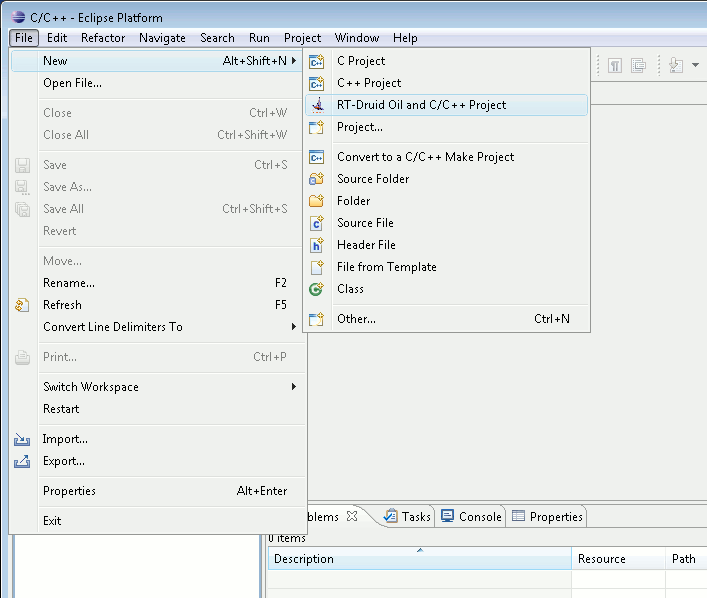
\includegraphics[width=8cm, bb=0 0 707 598]{images/project_new.png}
  \end{center}
  \caption{Activating the ``New Project'' Wizard.}
  \label{fig:rtdruid-project-new}
\end{figure}

After that, the wizard asks for a project template (see Figure
\ref{fig:rtdruid-project-template}), which is a pre-built application
that you can use, and after that for the project name and optionally
for the name of the home folder for the project. The use of spacing
characters in the project name is {\bf strongly discouraged} and
strictly forbidden for the names of all files inside the project
folder, since they would create problems with the
\file{make} and \file{gcc} tools when compiling a project, since (\file{make}
and \file{gcc} treat spaces as separators inside lists of file names
(see Figure \ref{fig:rtdruid-project-name}).

\begin{figure}
  \begin{center}
    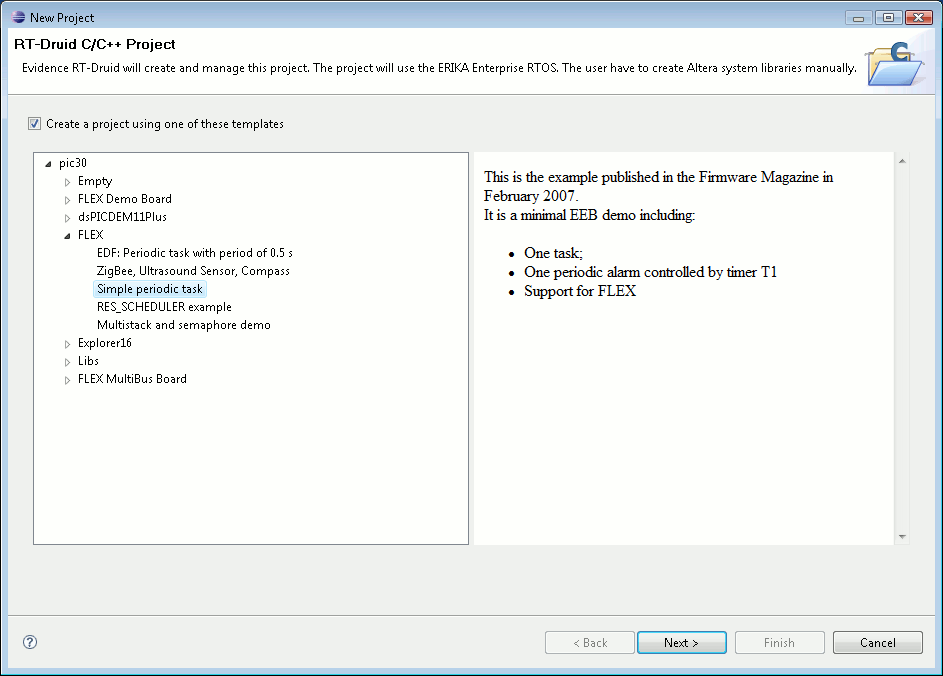
\includegraphics[width=8cm, bb=0 0 943 676]{images/project_template.png}
  \end{center}
  \caption{Choosing a template application for your new \rtd\ Project.}
  \label{fig:rtdruid-project-template}
\end{figure}

\begin{figure}
  \begin{center}
    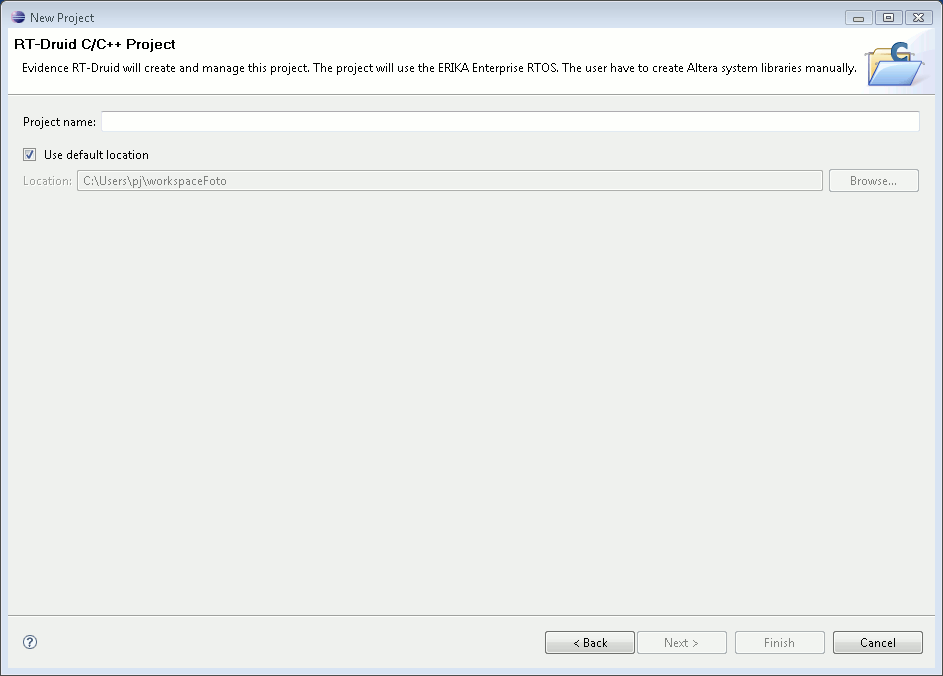
\includegraphics[width=8cm, bb=0 0 943 676]{images/project_name.png}
  \end{center}
  \caption{Choosing a  meaningful name for your new \rtd\ Project.}
  \label{fig:rtdruid-project-name}
\end{figure}

Once these steps are completed, the project is created and a OIL
configuration file template is automatically generated and inserted
into the project.

To edit the OIL File, just double click on in in the Navigation
sidebar, and a dedicated OIL Editor will appear.







\chapter{OIL syntax and OIL file generation}
\label{cha:oil-syntax}

OIL (OSEK Implementation Language) is a part of the OSEK/VDX standard,
that is used for OS and application configuration. The specification
of the OIL file structure and syntax is provided in the OSEK/VDX web
site at \url{http://www.osek-vdx.org} \cite{OSEKOIL}.

In the \rtd\ and in the \ee\ RTOS the configuration of the system is
defined inside an OIL file. In this chapter we only provide a quick
introduction of the OIL Language (see \cite{OSEKOIL} for a complete
description), together with a specification of the specific OIL
attributes implemented by \rtd.

Standard OIL has no knowledge of multiprocessor systems, nor of 
distribution of threads and resources. \ee\ provides mechanisms for 
resource sharing with predictable blocking time in a distributed 
environment. We defined a set of OIL extensions (see Section 
\ref{sec:oil-multicore}) which explicitly deals with the additional 
syntax features that are needed for the definition of a multiprocessor 
system, including placement of threads and resources. 

\section{OIL Basics}

In \ee\ all the RTOS objects like tasks, alarms, resources, are static
and predefined at application compile time. To specify which objects
exist in a particular application, \ee\ uses the OIL Language, which
is a simple text description language.

Here is an example of the OIL File for the \dspic\ device:

\begin{lstlisting}
CPU mySystem {
        OS myOs {
                EE_OPT = "DEBUG";
                CPU_DATA = PIC30 {
                        APP_SRC = "code1.c";
                        APP_SRC = "code2.c";
                        MULTI_STACK = FALSE;
                        ICD2 = TRUE;
                };

                MCU_DATA = PIC30 {
                        MODEL = 33FFJ256GP710;
                };

                BOARD_DATA = EE_FLEX {
                        USELEDS = TRUE;
                }

                KERNEL_TYPE = FP;
        };

        TASK myTask {
                PRIORITY = 1;
                STACK = SHARED;
                SCHEDULE = FULL;
        };

        TASK myTask {
                PRIORITY = 1;
                STACK = SHARED;
                SCHEDULE = FULL;
        };
};
\end{lstlisting}

The example contains a single object called \const{CPU}, which
contains all the specifications and the values used by the system. Inside
the \const{CPU}, are described the objects which are present in
the application: an \const{OS}, which specifies the global attributes
for the system, and, in the example, two \const{TASK}s.

The OIL File is parsed by the \rtd\ code generator and, as a result,
part of the RTOS source code is generated and compiled together with
the application.

An OIL file consists of two parts: a set of definitions and a set of
declarations. Definitions are used to define data types, constants and
kernel objects that need to be provided in the declaration part for
configuring a specific kernel. In other words, the definition part
tells the configurator that there exists different objects like
tasks, resources, and so on, describing their attributes and types,
like in a C struct declaration. Then, the declaration part is used to
specify which objects are really present in a particular application.

In \rtd, the definition part of the OIL file is fixed and is
contained inside the \rtd\ Eclipse Plugins. The definition part
including all the attributes which can be specified by users is
included in Appendix \ref{cha:oil-definition}. The user has only to
provide the declaration part, specifying for a particular application
the objects to be created.

The OIL file basically contains the description of a set of objects. A
\const{CPU} is a container of these objects. Other objects include the following:
\begin{itemize}
\item \const{OS} is the Operating System which runs on the CPU. This
  object contains all the global settings which influence the
  compilation process and the customization of the \ee\ RTOS.
\item \const{APPMODE} defines the different application mode.
  These modes are then used to control the autostart
  feature for tasks and alarms in the OIL file.
\item \const{TASK} is an application task handled by the OS.
\item \const{RESOURCE} is a resource (basically a binary mutex) used
  for mutual exclusion.
\item \const{EVENT} is a synchronization flag used by extended tasks.
\item \const{COUNTER} is a software source for periodic / one shot
  alarms.
\item \const{ALARM} is a notification mechanism attached to a counter
  which can be used to activate a task, set an event, or call a
  function.
\end{itemize}

All the attributes in the OIL file can be:

\begin{itemize}
\item numbers, i.e. the \const{PRIORITY} attribute;
\item strings, i.e. the \const{APP_SRC} attribute;
\item enumerations, i.e. the \const{KERNEL_TYPE} attribute.
\end{itemize}

Attributes can have a default value, as well as an {\em automatic}
value specified with the keyword \const{AUTO}. Some of the attributes
can be specified more than once in the OIL file, such as the
\const{APP_SRC}, and the configurator treats them as a {\em set} of
values; i.e., in the case of \const{APP_SRC}, the set of application
files to be compiled.

Finally, some items can in reality contain a set of sub-attributes,
like in a C-language struct definition. For example, \const{CPU_DATA}
contains a \const{PIC30} object, which is detailed by a set of
attributes.

\section{The CPU Object}

The CPU object is only used as a container of all the other objects,
and does not have any specific attribute.

\section{The OS Object}

The \oil{OS} Object is used to define the \ee\ global configuration as
well as the compilation parameters.

The attributes which can be specified for the \const{OS} object are 
specified in the following subsections.

\subsection{Compilation attributes}

The OIL file includes a set of fields for controlling the command line
parameters which are passed to the compiler tools. The meaning of those
elements is the following:

\begin{itemize}
\item \oil{EE_OPT} contains a list of additional compilation flags
  passed to the \ee\ makefile. In practice, the \const{EE_OPT}
  makefile variable controls which files has to be compiled and with
  which options. The \const{EE_OPT} attributes are translated in
  \const{#define}s in the C code.
\item \oil{CFLAGS} contains the list of additional C compiler options.
\item \oil{ASFLAGS} contains the list of additional assembly options.
\item \oil{LDFLAGS} Contains the list of additional linker parameters.
\item \oil{LDDEPS} Contains the list of additional library
  dependencies which have to be added to the makefile rules.
\item \oil{LIBS} Contains the list of additional libraries that needs
  to be linked.
\end{itemize}

Example of declaration:

\begin{lstlisting}
CPU mySystem {
  OS myOs {
    EEOPT = "MYFLAG1";
    EEOPT = "MYFLAG2";
    CFLAGS = "-G0";
    CFLAGS = "-O0 -g";
    CFLAGS = "-Wall -Wl,-Map -Wl,project.map";
    ASFLAGS = "-g";
    LIBS = "-lm";
    ...
  };
  ...
}
\end{lstlisting}

\subsection{OSEK attributes}
The OIL file includes a set of attributes which are part of the
OSEK/VDX specification. The meaning of those attributes is the
following:

\begin{itemize}
\item \oil{STATUS} specifies if the kernel should be compiled with
  \const{STANDARD} status or \const{EXTENDED} status. With the
  \const{STANDARD} status, only a subset of the error codes are 
  reported by the kernel primitives to reduce the system footprint. 
  This setting only applies to the OSEK/VDX conformance classes.
\item The settings \oil{STARTUPHOOK}, \oil{ERRORHOOK},
  \oil{SHUTDOWNHOOK}, \oil{PRETASKHOOK}, \oil{POSTTASKHOOK} specifies
  which particular hook routine should be included in the kernel.
\item \oil{USEGETSERVICEID} specifies if the Service ID debugging
  functionality of the \fn{ErrorHook()} routine should be included in
  the kernel.
\item \oil{USEPARAMETERACCESS} specifies if the \fn{ErrorHook()}
  should have access to the parameters passed to the primitives.
\item \oil{USERESSCHEDULER} specifies if the kernel includes the
  \const{RES_SCHEDULER} resource.
\end{itemize}

Example of declaration:

\begin{lstlisting}
CPU mySystem {
  OS myOs {
    STATUS = STANDARD;
    STARTUPHOOK = TRUE;
    ERRORHOOK = TRUE;
    SHUTDOWNHOOK = TRUE;
    PRETASKHOOK = FALSE;
    POSTTASKHOOK = FALSE;
    USEGETSERVICEID = FALSE;
    USEPARAMETERACCESS = FALSE;
    USERESSCHEDULER = TRUE;
    ...
  };
  ...
}
\end{lstlisting}

\subsection{Multi-core attributes}
The attributes \oil{STARTUPSYNC}, and \oil{USEREMOTETASK} are
described in the \ee\ Manual for the Altera Nios II target, since they
are specific for that architecture.

\subsection{Nios II target attributes}
The attributes \oil{NIOS2_MUTEX_BASE}, \oil{NIOS2_SYS_CONFIG},
\oil{NIOS2_APP_CONFIG}, \oil{IPIC_GLOBAL_NAME}, \oil{IPIC_LOCAL_NAME},
\oil{MP_SHARED_RAM}, \oil{MP_SHARED_ROM}, \oil{NIOS2_DO_MAKE_OBJDUMP},
\oil{SYSTEM_LIBRARY_NAME}, \oil{SYSTEM_LIBRARY_PATH}, \oil{NIOS2_PTF_FILE}, 
are described in the \ee\ Manual for the Altera Nios II target.

\subsection{CPU\_DATA sections}

The \oil{CPU_DATA} section of the \const{OS} object is used to specify
the configuration of a core in a single or in a multiple core device.

In general, the OIL file will contain a \const{CPU_DATA} section for
each core in the system. There is a specific \const{CPU_DATA} section
for each architecture supported by \ee. 

In particular, the \const{CPU_DATA} sections currently supported are
\oil{NIOSII}, \oil{PIC30} and \const{AVR_5}, which contain the following
attributes:

\begin{itemize}
\item \oil{ID} is a symbolic name uniquely identifying the
  CPU. The name used for the \const{CPU_ID} attribute must be the same
  name that is used when allocating objects to a particular CPU.

  CPUs with no name automatically get a default name
  \const{default_cpu}\index{default\_cpu}. If more than one CPU gets
  \const{default_cpu}, an error is raised, because different CPUs
  cannot have the same name.

  \const{default_cpu} is subsumed also when allocating Tasks (see
  Section \ref{sub:task-mapping-to-cpu}), and counters (see Section
  \ref{sec:counter-extensions}) to a CPU, and when the Master CPU is
  assigned (see Section \ref{sub:master-cpu}).

  For single processor systems, it is safe to avoid any declaration of
  the \const{CPU_ID} field in the entire OIL file. In this way, all
  the objects will be mapped to the only CPU in the system, named
  \const{default_cpu}.

  Example of declaration:

\begin{lstlisting}
CPU mySystem {
  OS myOs {
    CPU_DATA = NIOSII {
      ID = "mycpu";
      ...
    }
    ...
  };
  ...
}
\end{lstlisting}

\item \oil{APP_SRC} declares a list of all files containing code to
  be executed on the CPU.

  Example of declaration:

\begin{lstlisting}
CPU mySystem {
  OS myOs {
    CPU_DATA = NIOSII {
      APP_SRC = "file1.c";
      APP_SRC = "file2.c";
      ...
    }
    ...
  };
  ...
}
\end{lstlisting}


\item \oil{MULTI_STACK} defines if the system supports multiple
  stacks for the application tasks (\const{TRUE}) or not
  (\const{FALSE}). The default value is \const{FALSE}.

  If set to \const{TRUE}, it is possible to specify if IRQs are
  executed using a dedicated stack space. The attribute
  \oil{IRQ_STACK} is used for this purpose.

  Some architectures also allow the specification of a
  \oil{DUMMY_STACK}, which specifies if the background task is using
  a shared stack (\const{SHARED} value) or a dedicated stack segment
  (\const{PRIVATE} value). \ee\ schedules the \fn{main()}
  function as a background task, also called ``dummy'' task. For
  example, the Altera Nios II architecture provides support for the
  above described mechanism, while the \dspic\ family does not support
  it.

\item \oil{STACK_TOP} contains the highest address from which the
  stack space starts. The address can be provided as a symbol,
  assuming that the symbol is associated to a value in some other part
  of the OIL declaration or in some application file. For example, in
  the Altera Nios II HW version of \ee, the typical value for this
  attribute is \const{__alt_stack_pointer}, that is the symbol used
  inside the Altera Nios II System libraries as the initial stack
  pointer.

\item \oil{SYS_SIZE} is used to declare the total size of the memory
  that is allocated to the task stacks.

\item \oil{SHARED_MIN_SYS_SIZE} used to declare the minimum size of
  the shared stack space. The dimension of the shared stack space is
  computed as the difference between the available space
  (\const{SYS_SIZE}) and the space required for implementing the private
  stack spaces. \rtd\ guarantees that the remaining size is higher
  than or equal to the value defined with the
  \const{SHARED_MIN_SYS_SIZE} directive (an error is raised
  otherwise). The default value for this attribute is zero.

\item The attributes \oil{ICD2} and \oil{ENABLE_SPLIM} are described
  in the \ee\ Manual for the Microchip PIC24, dsPIC30 (R) DSC and
  dsPIC33 (R) DSC targets.

\item The specific attributes about the \oil{AVR_5} architecture are
  described in the \ee\ Manual for the Atmel AVR5 targets.
\end{itemize}

Here is an example of a declaration of a Nios II \const{CPU_DATA}:

\begin{lstlisting}
CPU mySystem {
  OS myOs {
    CPU_DATA = NIOSII {
      ID = "cpu2";
      MULTI_STACK = TRUE {
	IRQ_STACK = FALSE;
	DUMMY_STACK = SHARED;
      };
      APP_SRC = "cpu2_startup.c";
      STACK_TOP = 0x20004000;
      SHARED_MIN_SYS_SIZE = 1800;
      SYS_SIZE = 0x1000; 
      IPIC_LOCAL_NAME = "IPIC_INPUT_CPU0";
    };
    ...
  };
  ...
}
\end{lstlisting}

The same example can be written in two stages by splitting the
declaration of the structure. The only requirement is that the
separate declarations do not contain any conflicting assignment to the
same field name. The previous example can be rewritten as follows:

\begin{lstlisting}
CPU mySystem {
  OS myOs {
    CPU_DATA = NIOSII {
      ID = "cpu2";
      MULTI_STACK = TRUE {
	IRQ_STACK = FALSE;
	DUMMY_STACK = SHARED;
      };
      APP_SRC = "cpu2_startup.c";
    };
    
    CPU_DATA = NIOSII {
      ID = "cpu2";
      STACK_TOP = 0x20004000;
      SHARED_SYS_SIZE = 1800;
      SYS_SIZE = 0x1000; 
      IPIC_LOCAL_NAME = "IPIC_INPUT_CPU0";
    };
    
    CPU_DATA = NIOSII {
      /* The ID is not defined, this section refers
         to the "default_cpu" */
      STACK_TOP = "alt_data_end";
    };
    ...
  };
  ...
}
\end{lstlisting}

%\item [ARM7]
%
%  In case of an ARM7 target, the declaration of a stack space requires
%  both \const{SYS\_SIZE} e \const{IRQ\_SIZE}, for the system and IRQ
%  stack, respectively.

\subsection{MCU\_DATA sections}

The \oil{MCU_DATA} section of the \const{OS} object is used to specify
the configuration of peripherals which are present in a specific
microcontroller.

The following microcontrollers are supported:
\begin{itemize}
\item Microchip PIC24 microcontrollers and dsPIC DSCs. Please refer to
  the \ee\ Manual for the Microchip PIC24, dsPIC30 (R) DSC and dsPIC33
  (R) DSC targets.
\end{itemize}

\subsection{BOARD\_DATA sections}

The \oil{BOARD_DATA} section of the \const{OS} object is used to
specify the configuration of the board where the microcontroller is
placed. For example, the board configuration includes the
configuration of the external devices like leds, buttons, displays,
and other peripherals.

The following boards are supported:
\begin{itemize}
\item \oil{NO_BOARD} is a placeholder to specify that no board
  configuration is required.
\item \oil{EE_FLEX} is the Evidence / Embedded Solutions \flex\ Board
  based on the Microchip \dspic. For details, please refer to the
  \ee\ Manual for the Microchip PIC24, dsPIC30 (R) DSC and dsPIC33 (R)
  DSC targets.
\item \oil{MICROCHIP_EXPLORER16} is the Microchip Explorer 16
  evaluation board. For details, please refer to the \ee\ Manual for the
  Microchip PIC24, dsPIC30 (R) DSC and dsPIC33 (R) DSC targets.
\item \oil{MICROCHIP_DSPICDEM11PLUS} is the Microchip dsPIC Demo Plus
  1.1 evaluation board. For details, please refer to the \ee\ Manual
  for the Microchip PIC24, dsPIC30 (R) DSC and dsPIC33 (R) DSC
  targets.
\item \oil{ATMEGA_STK50X} is the Atmel STK 500 evaluation board for
  the AVR5 architecture. For details, please refer to the \ee\ Manual
  for the Atmel AVR5 targets.
\item \oil{XBOW_MIB5X0} is the Crossbow MIB 5x0 board used to program
  wireless sensor network hardware. For details, please refer to the
  \ee\ Manual for the Atmel AVR5 targets.
\end{itemize}

\subsection{Library configuration}
Typical microcontroller applications needs to link external libraries
to the application code. \ee\ supports both the linking of external
binary libraries as well as the development of library code that can
be automatically built by the \ee\ build scripts.

\subsubsection{Linking an external third-party binary library}
A third-party binary library is typically provided as a binary archive
with a ``.a'' extension.

If you need to link this kind of library to your executable, just add
the following lines to the OIL file:
\begin{lstlisting}
  CPU mySystem {
    OS myOs {
      LDFLAGS = "-Llibrarypath";
      LIBS = "-llibraryname";
    };
  };
\end{lstlisting}

These lines have the effect to add the proper option to tell the
linker to load the library you specified.

\subsubsection{Building and using libraries which are integrated in the \ee\ build system}

In this case, the target is to use the library code which is provided
in the \ee\ build tree. Basically, the OIL file can specify a set of
libraries which are distributed with or are supported by \ee\ and that
have to be linked together with the application. The specification is
done by using the \oil{LIB} attribute.

An example of this kind of library are the Scicos library, and other
communication libraries which can be found under the \file{ee/contrib}
directory of the \ee\ source tree.

The list of supported libraries depends on the target and
can be found in the \ee\ Manual for the specific target. 

The \const{LIB} attribute can be used in one of the following ways:

\begin{itemize}

\item
  This first option helps to build the library files -only-. In
  particular, \const{LIB} can be used to specify an OIL file which
  only compiles the supported libraries (that is, the OIL file is used
  to configure the libraries but {\em not} the application). The
  following example is an OIL file which only compiles the library
  \file{mylib.a}:

\begin{lstlisting}
  CPU mySystem {
    OS myOs {
      EE_OPT = "__BUILD_LIBS__";
      LIB = ENABLE { NAME = "mylib"; };
      CPU_DATA = PIC30;
    };
  };
\end{lstlisting}

\begin{note}
To compile {\em all} the libraries that are supported by a particular
architecture with a single OIL file, the following OIL file
configuration can be used:

\begin{lstlisting}
  CPU mySystem {
    OS myOs {
      EE_OPT = "__BUILD_ALL_LIBS__";
      CPU_DATA = PIC30;
    };
  };
\end{lstlisting}

\end{note}


\item
  \const{LIB} can be used for the {\em on-the-fly} creation of the
  library during the application compilation process. That is, the
  build process will create the library as well as the \ee\ library
  \file{libee.a}. After that, the application code will be compiled
  and linked with all the libraries just created. The following
  example can be used to compile and link the library \file{mylib.a}.

\begin{lstlisting}
  CPU mySystem {
    OS myOs {
      EE_OPT = "__ADD_LIBS__";
      LIB = ENABLE { NAME = "mylib"; };
      ...
    };
    ...
  };
\end{lstlisting}

\item
  In this case, an application will be linked with a library which has
  been generated using a separate OIL file. The following example
  shows the OIL file which can be used to link an already existing
  library which is located in the directory
  \file{librarypath}. \file{librarypath} typically is the \file{Debug}
  directory of a project used to build a library, as explained in the
  first bulled of this list.

\begin{lstlisting}
  CPU mySystem {
    OS myOs {
      LDFLAGS = "-Llibrarypath";
      LIB = ENABLE { NAME = "mylib"; };
      ...
    };
    ...
  };
\end{lstlisting}

\item
  Finally, please note that more than one library can be specified in
  a OIL file in one of the following two ways:
\begin{lstlisting}
  CPU mySystem {
    OS myOs {
      LIB = ENABLE { NAME = "mylib1"; };
      LIB = ENABLE { NAME = "mylib2"; };
      LIB = ENABLE { NAME = "mylib3"; };
      ...
    };
    ...
  };

  CPU mySystem {
    OS myOs {
      LIB = ENABLE {
	NAME = "mylib1"; 
	NAME = "mylib2"; 
	NAME = "mylib3"; 
      };
      ...
    };
    ...
  };
\end{lstlisting}

\end{itemize}


\subsection{Kernel Conformance class}

An explicit declaration of the kernel conformance class is required in
the \oil{KERNEL_TYPE} definition. The definition is shown below:

\begin{lstlisting}
  ENUM [
    FP {
      BOOLEAN NESTED_IRQ;
    },
    EDF {
      BOOLEAN NESTED_IRQ;
      STRING TICK_TIME; 
      BOOLEAN REL_DEADLINES_IN_RAM = FALSE;
    },
    FRSH {
      ENUM [
	CONTRACT {
	  STRING NAME;
          UINT32 BUDGET;
	  UINT32 PERIOD;
	  STRING CPU_ID;
        }
      ] CONTRACTS[];
      BOOLEAN USE_SYNC_OBJ;
      STRING TICK_TIME;
    },
    BCC1,
    BCC2,
    ECC1,
    ECC2
  ] KERNEL_TYPE;
\end{lstlisting}

For the \const{EDF} and \const{FRSH} kernels, it is possible to
specify the tick length. Given the tick length for the circular timer,
which is then used to compute the values to put in the relative
deadline task parameter. The tick time can be specified in various
unit measures, such as seconds (``s''), milliseconds (``ms''),
microseconds (``us''), and nanoseconds (``ns''). Please check the
manual for the CPU architecture you are currently using for the proper
configuration of the tick parameter. The EDF kernel has an additional
option which allows to specify that relative deadlines should be
stored in RAM and not in Flash, to allow them to be changed at
runtime.

For the \const{FRSH} kernel\footnote{The FRSH kernel is the result of
the IST FP6 FRESCOR Project, \url{http://www.frescor.org}}, a set of
contracts have to be specified. For each contract, the user has to
specify the contract name, the budget and period (either in clock
ticks or using unit measures as for the tick time described above),
and the \const{CPU_ID} (which must only be specified on multicore
applications).

For more details on the \const{FRSH} kernel, please see
% *** broken sentence

Some examples of use within the declaration part are the following:

\begin{enumerate}

\item
  To configure the \const{BCC1} conformance class:
  \begin{lstlisting}
    KERNEL_TYPE = BCC1;
  \end{lstlisting}
  
\item
  To configure the \const{FP} conformance class: 
  
  \begin{lstlisting}
    KERNEL_TYPE = FP;
  \end{lstlisting}
  
  By default, nested IRQs are set to \const{FALSE}.
  
\item
  To configure the \const{EDF} conformance class:
  
  \begin{lstlisting}
    KERNEL_TYPE = EDF { 
      NESTED_IRQ = TRUE; 
      TICK_TIME = "10.5ns"; 
      REL_DEADLINES_IN_RAM = TRUE;
    };
  \end{lstlisting}
  
  Nested IRQs are set to \const{TRUE}.

\item
  To configure the \const{FRSH} conformance class:
  
  \begin{lstlisting}
    KERNEL_TYPE = FRSH {
      TICK_TIME = "20ns";
      USE_SYNC_OBJ = TRUE;
      CONTRACTS = CONTRACT {
	CPU_ID = "cpu1";
        NAME = "c1";
        BUDGET = 20000;
        PERIOD = 100000;
      };
      CONTRACTS = CONTRACT {
	CPU_ID = "cpu3";
        NAME = "c7";
        BUDGET = "10ms";
        PERIOD = "50ms";
      };
    };
  \end{lstlisting}

  In this case, the \const{FRSH} kernel is configured with two
  contracts on different CPUs. budget and period are specified either
  with a unit measure or with clock cycles.
  
\end{enumerate}



\subsection{ORTI file generation and kernel awareness with Lauterbach Trace32}
\label{sub:orti}
% ripreso in buona parte dall'event demo...

This section describes the steps to use the Lauterbach Trace32 ORTI
support in \ee. To generate the ORTI information, the
\oil{ORTI_SECTIONS} attribute has to be specified inside the
\const{OS} object. The definition of \const{ORTI_SECTIONS} is the following:

\begin{lstlisting}
  ENUM [
    NONE,
    ALL,
    OS_SECTION,
    TASK_SECTION,
    RESOURCE_SECTION,
    STACK_SECTION,
    ALARM_SECTION
  ] ORTI_SECTIONS[];
\end{lstlisting}

Basically, each ORTI section can be selected separately. If
\const{ALL} is specified, then all the ORTI sections are generated.

Notice that the ORTI support currently applies only to the Altera Nios
II target for the \const{BCC1}, \const{BCC2}, \const{ECC1},
\const{ECC2}, \const{FRSH} conformance classes.

\rtd\ provides the possibility to automatically generate an
ORTI\footnote{ORTI is a standard file format specified by the OSEK/VDX
consortium.} file.  An ORTI file is basically a text file that
specifies which data structures the kernel information are stored
in. The file is parsed by an ORTI--enabled debugger, providing useful
feedback to the application developer during debug sessions.

Also, \rtd\ automatically produces a set of scripts that can be used
to automatically launch a Lauterbach Trace32 debugger
\cite{Lauterbach}. The provided scripts automatically load the FPGA
hardware, and start a debug session for each CPU in the system.

To enable all these features, you need to specify a JAM file
name\footnote{JAM is one of the file formats containing the FPGA
configuration that is accepted by Lauterbach Trace32} inside the OS
section of the OIL file, as well as the specification of the ORTI
sections that should be generated, as follows:

\begin{lstlisting}
CPU test_application {
  OS EE {
    ...
    NIOS2_JAM_FILE = "JAM_filename.jam";
    ORTI_SECTIONS = ALL;
  }
  ...
}
\end{lstlisting}

In the above example, \const{ALL} causes the generation of all the
ORTI information, and \file{JAM_filename.jam} is the path name of 
the JAM file specified in the \oil{NIOS2_JAM_FILE} attribute. If not
specified, \file{../../fpga.jam} is used.

As a result of the compilation process, a set of files are produced
inside the \file{Debug} directory (see Table \ref{tab:t32files} for a
detailed list).

Please refer to Section \ref{sec:trace32} for information on how to
use the ORTI Files and launch a Lauterbach Trace32 session.

%
\begin{table}
\begin{center}
\begin{tabular}{|c|p{8cm}|}
\hline 
File name&
Description\tabularnewline
\hline
\hline 
\file{debug.bat}&
This batch script loads the FPGA hardware and starts a T32 instance
for each CPU. You can double click it on the Nios II IDE to directly
launch the debug session.\tabularnewline
\hline 
\file{debug\_nojam.bat}&
This batch script starts a T32 instance for each CPU. You can double
click it on the Nios II IDE to directly launch the debug session.
You can use it if the FPGA has been already programmed with the hardware
contents.\tabularnewline
\hline 
\file{t32.cmm}&
Main PRACTICE script, responsible for loading the JAM file and starting
all the T32 instances on every CPU.\tabularnewline
\hline 
\file{testcase\_data.cmm}&
Internal file used for automatic testcase generation.\tabularnewline
\hline 
\file{t32/{*}}&
Internal PRACTICE scripts. They are a copy of the files inside 
\file{components/evidence\_ee/ee/pkg/cpu/nios2} 
\file{/debug/lauterbach/t32}.\tabularnewline
\hline 
\file{cpuname/config.t32}&
Configuration file for T32. Contains the Multicore configuration 
information.\tabularnewline
\hline 
\file{cpuname/orti.men}&
Trace32 menu automatically generated using the Lauterbach ORTI menu
generator.\tabularnewline
\hline
\file{cpuname/system.orti}&
The ORTI file, for each CPU.\tabularnewline
\hline
\file{cpuname/t32.cmm}&
The main script file executed by each CPU.\tabularnewline
\hline
\end{tabular}
\end{center}

\caption{\label{tab:t32files} Files generated for the Lauterbach
Trace32 support. ({\em cpuname} represents the name of the CPU as specified 
in the OIL file).}
\end{table}


\section{The Application mode Object}
The \oil{APPMODE} object is contained by the \const{CPU} object and is
used to define an application mode.

Example:

\begin{lstlisting}
CPU test_application {
  ...
  APPMODE myAppMode1;
  APPMODE myAppMode2;
  APPMODE myAppMode3;
  ...
}
\end{lstlisting}




\section{The Task Object}

The \oil{TASK} object is contained inside the \const{CPU} object and it is used to specify the properties of a task.

\subsection{Autostart attribute}
The \oil{AUTOSTART} attribute specifies if the task should be
automatically activated at system startup by the \fn{StartOS()}
primitive.

If the task must be activated at startup, the \const{AUTOSTART}
attribute has a value \const{TRUE}. When \const{TRUE}, the
\const{APPMODE} sub-attribute lists the application modes for which
the task is autostarted.

Example:

\begin{lstlisting}
CPU test_application {
  ...
  TASK myTask1 {
    AUTOSTART = TRUE { APPMODE = myAppMode1; };
    ...
  };
  TASK myTask2 {
    AUTOSTART = FALSE;
    ...
  };
  ...
}
\end{lstlisting}

\subsection{Priority attribute}
In the FP kernel, the \oil{PRIORITY} attribute specifies the task
priority. In the EDF kernel, the value specifies the task preemption
level. The value is used by \rtd\ as a relative ordering of priorities
and not as an absolute priority value. Higher values correspond to
higher priorities.

Example:

\begin{lstlisting}
CPU test_application {
  ...
  TASK myTask1 {
    PRIORITY = 1;
    ...
  };
  ...
}
\end{lstlisting}

\subsection{Relative Deadline attribute}
The \oil{RELDLINE} attribute specifies the task relative deadline. The
value is used by \rtd\ to compute the numerical value of the timing
attribute. The value can be expressed as a timing quantity such as
seconds (``s''), milliseconds (``ms''), microseconds (``us''), or
nanoseconds (``ns''). The value is interpreted as a time, and it is
divided by the \const{TICK_TIME} attribute specified inside the OS
attribute \const{KERNEL_TYPE} to obtain the final tick value which is
then programmed inside the microcontroller.

If a number is specified without any time unit (e.g., ``1234'' and not
``1234ms''), then the number is taken ``as is'' and programmed to
the target device.

Please remember that, to be complete, the OIL
file should also include a specification of the preemption level of
the task by using the \const{PRIORITY} field.

Example:

The following example specifies the preemption level and the relative
deadline of an EDF task.

\begin{lstlisting}
CPU test_application {
  OS myOS {
    ...
    KERNEL = EDF;
  };
  ...
  TASK myTask1 {
    PRIORITY = 3;
    REL_DEADLINE = "10ms";
    ...
  };
  ...
  TASK myTask2 {
    PRIORITY = 4;
    REL_DEADLINE = "1234";
    ...
  };
  ...
}
\end{lstlisting}


\subsection{Activation attribute}
The \oil{ACTIVATION} attribute specifies the number of pending
activations which can be stored by a task. It is only used in the
\const{BCC1}, \const{BCC2}, \const{ECC1}, and \const{ECC2} conformance
classes.

Example:

\begin{lstlisting}
CPU test_application {
  ...
  TASK myTask1 {
    ACTIVATION = 3;
    ...
  };
  ...
}
\end{lstlisting}

\subsection{Schedule attribute}
The \oil{SCHEDULE} attribute specifies if a task is full preemptive
(\const{FULL}) or non preemptive (\const{NON}).  The default is \const{NON}.

Example:

\begin{lstlisting}
CPU test_application {
  ...
  TASK myTask1 {
    SCHEDULE = FULL;
    ...
  };
  TASK myTask2 {
    SCHEDULE = NON;
    ...
  };
  ...
}
\end{lstlisting}

\subsection{Event attribute}
The \oil{EVENT} attribute is used to list the Events which belong to
a task. It is used in conformance classes \const{ECC1} and
\const{ECC2}.

Example:

\begin{lstlisting}
CPU test_application {
  ...
  TASK myTask1 {
    EVENT = "TimerEvent";
    EVENT = "ButtonEvent";
    ...
  };
  ...
}
\end{lstlisting}

\subsection{Resource attribute}
The \oiltwo{RESOURCE}{RESOURCEtask} attribute is used to list the
Resources used by a task.

Example:

\begin{lstlisting}
CPU test_application {
  ...
  TASK myTask1 {
    RESOURCE = "Resource1";
    RESOURCE = "Resource2";
    ...
  };
  ...
}
\end{lstlisting}


\subsection{Contract attribute}
The \oiltwo{CONTRACT}{CONTRACTtask} attribute is used to specify the \const{CONTRACT} statically linked to the task. The \const{CONTRACT} name must be one of the contracts listed in the \const{FRSH} \refoillst{KERNEL_TYPE}! section.

Example:

\begin{lstlisting}
CPU test_application {
  ...
  TASK myTask1 {
    CONTRACT = "Contract1";
    ...
  };
  ...
}
\end{lstlisting}

\subsection{Stack attribute}
The \oil{STACK} attribute is used to specify if the task stack is shared or of the task should have a separate private stack.

Example:

\begin{lstlisting}
CPU test_application {
  ...
  TASK myTask1 {
    STACK = SHARED;
    ...
  };
  TASK myTask2 {
    STACK = PRIVATE {
      SYS_SIZE = 128;
    };
  };
  ...
}
\end{lstlisting}

\subsection{Mapping tasks to CPUs using the CPU ID attribute}
\label{sub:task-mapping-to-cpu}

The \oiltwo{CPU_ID}{CPU_IDtask} attribute is used to specify the CPU
to which the task is allocated. The placement of the tasks on the CPUs
is defined before the compile time and can not be changed during the
system execution time. If the CPU identifier is missing, then \rtd\
assumes the default value ``default\_cpu''. An error is generated if
the CPU identifier specified for the task does not exist in the
system.

Example:

\begin{lstlisting}
CPU test_application {
  ...
  TASK myTask1 {
    CPU_ID = "cpu1";
    ...
  };
  ...
}
\end{lstlisting}



\subsection{Source files for each CPU}
The source files implementing the tasks can be declared inside the OIL
file in a dedicated section named \oiltwo{APP_SRC}{APP_SRCtask}. This allows identification of the
required files when producing the executable code for each CPU. The
\file{makefile} is automatically generated based on this declaration,
so that only the files implementing the task executing on the CPU need
to be compiled. If the task is moved to another CPU, the makefile is
automatically updated.

Example of declaration:

\begin{lstlisting}
CPU mySystem {
  TASK myTask {
    APP_SRC = "file1.c";
    APP_SRC = "file2.c";
    ...
  }
  ...
}
\end{lstlisting}

\subsection{Intertask notifications}
\label{sec:intertask-notifications}
The attribute \oil{LINKED} is related to intertask notifications on
multicore architectures and is described in the \ee\ Manual for the
Altera Nios II target.





\section{The Resource Object}

The \oil{RESOURCE} object is contained inside the \const{CPU} object
and it is used to specify the properties of a resource.

The Resource object contains an attribute named \oil{RESOURCEPROPERTY}
which can take the following values: 
\begin{itemize}
\item \const{STANDARD} is the default used for a normal resource. In
  that case, a set of source files can be specified using the
  \const{APP_SRC} sub-attribute. These files typically contain the
  resource data definition.
\item \const{LINKED} resources are only links/alias for other
  resources.
\item \const{INTERNAL} resources are currently not implemented.
%used for stack sharing techniques
%, only \const{STANDARD} type resources require the
%declaration of the source files implementing them. Please note that on
%a multiprocessor system \const{INTERNAL} resources can only be
%local. Global Internal resources are forbidden.
\end{itemize}

Example:

\begin{lstlisting}
CPU mySystem {
  RESOURCE mutex {
    RESOURCEPROPERTY = STANDARD {
      APP_SRC = "shareddata.c";
    };
  };
  ...
};
\end{lstlisting}

\section{The Event Object}
The \oiltwo{EVENT}{EVENTobj} object is used to define a bit mask which
then can be used by extended tasks. Events with the same name are
identical, and have the same mask. Events with the same mask are not
identical. If the value \const{AUTO} is specified for a mask, then
\rtd\ automatically computes the mask value.

Example:

\begin{lstlisting}
CPU mySystem {
  EVENT myEvent1 {
    MASK = 0x01;
  };
  EVENT mtEvent2 {
    MASK = AUTO;
  };
  ...
};
\end{lstlisting}



\section{The Counter object}
\label{sec:counter-extensions}

The \oil{COUNTER} object is the timing reference that is used by alarms.

The attributes of a counter are the following:
\begin{itemize}
\item \const{CPU_ID} is an indication
  of the CPU on which the counter is mapped. The default value is
  \const{default\_cpu}. If the identifier of the CPU does not exist in
  the system, an error is generated.
\item \const{MINCYCLE} is currently ignored by \ee.
\item \const{MAXALLOWEDVALUE} is currently ignored by \ee.
\item \const{TICKSPERBASE} is currently ignored by \ee.
%
% toOl: che significa che vengono ignorati?!?
%
\end{itemize}

Example:

\begin{lstlisting}
CPU mySystem {
  COUNTER myTimer {
    MINCYCLE = 32;
    MAXALLOWEDVALUE = 127;
    TICKSPERBASE = 23;
  };
  ...
};
\end{lstlisting}

\section{The Alarm Object}

The \oil{ALARM} Object is used to implement an asynchronous
notification which can activate a task, set an event or call a
callback function. Alarms can be autostarted at boot time depending on
the application mode.

The attributes of an alarm are the following:
\begin{itemize}
\item \const{COUNTER} specifies the counter to which the alarm is
  statically linked.
\item \const{ACTION} specifies the kind of action which has to be
  implemented when the alarm fires. The action is specified using one
  of the following sub-attributes:
  \begin{itemize}
  \item \const{ACTIVATETASK} specifies that a task has to be
    activated. The name of the task must be specified inside the
    \const{TASK} sub-attribute.
  \item \const{SETEVENT} specifies that an event has to be set on a
    task. The task name and event must be specified inside the
    \const{TASK} and \const{EVENT} sub-attributes.
  \item \const{ALARMCALLBACK} specifies that an alarm callback has to
    be called. The name of the callback is specified inside the
    attribute \const{ALARMCALLBACKNAME}.
  \end{itemize}
\item \const{AUTOSTART} specifies if the alarm has to be autostarted
  at system startup. If \const{TRUE}, the alarm properties and the
  application modes for which the alarm should be autostarted have to be
  specified in the sub-attributes \const{ALARMTIME}, \const{CYCLETIME},
  and \const{APPMODE}.
\end{itemize}

\section{Notes on source files}

If a system object (CPU, TASK or RESOURCE) is implemented by more than
one source file, all the corresponding file names need to appear in
one or more corresponding OIL declarations (not necessarily in order,
as shown by the following examples for a CPU, a task and a resource):

\begin{lstlisting}
  CPU_DATA = NIOSII {
    ID = "cpu0";
    APP_SRC = "cpu0_src0.c";
  };
  CPU_DATA = NIOSII {
    ID = "cpu0";
    APP_SRC = "cpu0_src1.c";
    APP_SRC = "cpu0_src2.c";
    APP_SRC = "cpu0_src3.c";
    APP_SRC = "cpu0_src4.c";
  };
\end{lstlisting}

\begin{lstlisting}
  TASK thread1 {
    CPU_ID = "cpu1";
    APP_SRC = "thread1_a.c";
    APP_SRC = "thread1_b.c";
    APP_SRC = "thread1_c.c";
  };
\end{lstlisting}

\begin{lstlisting}
  RESOURCE mutex {
    RESOURCEPROPERTY = STANDARD {
      APP_SRC = "res_a.c";
      APP_SRC = "res_b.c";
    };
  };
\end{lstlisting}

It is possible, even if we discourage its use, to list several file
names in the same declaration, separated by spaces:

\begin{lstlisting}
  APP_SRC = "cpu0_src1.c cpu0_src2.c";
\end{lstlisting}

If a file name appears more than once, all declarations following the
first one are ignored.

\section{OIL extensions for multiprocessing}
\label{sec:oil-multicore}

\subsection{Partitioning support}
When developing a multiprocessor application, the developer faces the
job of mapping a multitask application on the CPUs that are available
in the system.  That mapping procedure involves the partitioning of
the application tasks into the CPUs, meeting all application
constraints.

As the starting point, each CPU runs a copy of \ee, and all the copies 
of \ee\ on the CPUs have the same configuration. Depending on the 
application needs, for example, the kernel can be configured to have 
monostack or multistack support, which is useful when dealing with 
blocking primitives, and to support debugging features such as hooks, 
and extended error status report. All these features are set at the same 
time for all CPUs. For example, the case where a CPU runs with monostack 
support while other CPUs run with multistack support is not possible. 

From the OIL configuration point of view, the developer defines a set
of CPUs in the OIL configuration file using the \const{CPU_DATA}
sections inside the \const{OS} object, and the job of partitioning
consists in placing the OIL objects into the existing CPUs.

The OIL Objects that must be explicitly mapped to a processor are
Tasks and Counters. As explained in Sections
\ref{sub:task-mapping-to-cpu} and \ref{sec:counter-extensions} the OIL
extensions implemented by \rtd\ allow the specification of the CPU to
which a \const{TASK} or \const{COUNTER} is allocated by using the
attribute \const{CPU_ID}. The link between the particular object (Task
or Counter) and the CPU is {\em static} and specified at compile time,
and cannot be changed at runtime.

Other OIL Objects are automatically mapped by the system. In
particular, Resources will be {\em local} if the tasks using them are
allocated to the same CPU or {\em global} otherwise. Alarms are linked
to a Counter (that in turn is mapped to a CPU). However, please note
that Alarm notifications can result in activation of remote tasks, and
setting of events on remote tasks.

Finally, other objects are local and are replicated on each CPU. Hooks
and Application Modes fall in this category. This means that each CPU
will have its own copy of the hook routines, and each CPU will be
initialized passing an appropriate Application Model. It is
responsibility of the application developer that all CPUs are
initialized with the same Application mode.


\subsection{Master CPU}
\label{sub:master-cpu}
%
%\nb{PJ: questo lo ho spiegato bene anche nella parte multiprocessore,
%forse conviene riprenderlo da li o citare quello!!!}
%

When designing multiprocessor systems, the user must specify which CPU
acts as ``Master CPU''\footnote{For details about the role of the Master CPU
please look at the Multiprocessor Sections of the \ee\ manuals}. Here
is the definition of the \oil{MASTER_CPU} attribute:

\begin{lstlisting}
  STRING MASTER_CPU = "default_cpu";
\end{lstlisting}

The default value for the \const{MASTER_CPU} attribute is
\const{default_cpu}\index{default\_cpu}. 

Example:
\begin{lstlisting}
  MASTER_CPU = "cpu0";
\end{lstlisting}




\subsection{Specification of the source files.}

In order to make easier the change among different application 
partitionings, each
system object should be implemented in a separate file. Then, each
file is specified into the OIL file as the implementation of the
corresponding object, such as \const{CPU_DATA}, \const{TASK},
\const{RESOURCE}. \rtd\ uses the information to create the
\file{subdir.mk} files that are used by the makefile scripts to
compile the source code.

\rtd\ generates a \file{subdir.mk} file for each CPU, including all
the files that refer to the objects allocated to the CPU.

When a source file is specified inside a \const{CPU_DATA} element, the
file is inserted in the \file{subdir.mk} of that CPU.

When a source file is specified inside a \const{TASK} element, the
file is inserted in the CPU where the task is allocated.

When a source file is specified inside a \const{RESOURCE} element, the
file is inserted in the CPU where all the tasks using it are allocated
in case it is a local resource, or on the Master CPU if it is a global
resource.

A source file name can be specified more than once inside the OIL
file. However, it will be inserted at most once for each CPU.

To better understand this situation, consider the following example:

\begin{lstlisting}
CPU test_application {

  OS EE {
    MASTER_CPU = "cpu0";			

    CPU_DATA = NIOSII {
      ID = "cpu0";
      APP_SRC = "cpu0.c";
    };

    CPU_DATA = NIOSII {
      ID = "cpu1";
      APP_SRC = "cpu1.c";
    };
  };

  TASK task0 {
    CPU_ID = "cpu0";
    APP_SRC = "task0.c";
    RESOURCE = globalmutex;
  };

  TASK task1 {
    CPU_ID = "cpu1";
    APP_SRC = "task1.c";
    RESOURCE = globalmutex;
    RESOURCE = localmutex;
  };

  TASK task2 {
    CPU_ID = "cpu1";
    APP_SRC = "task2.c";
    RESOURCE = localmutex;
  };
  
  RESOURCE globalmutex {
    RESOURCEPROPERTY = STANDARD { APP_SRC = "globalmutex.c"; };
  };

  RESOURCE localmutex {
    RESOURCEPROPERTY = STANDARD { APP_SRC = "localmutex.c"; };
  };
};
\end{lstlisting}

\const{cpu0}'s \file{subdir.mk} will include the files
\file{cpu0.c}, \file{task0.c}, and \file{globalmutex.c};
\const{cpu1}'s \file{subdir.mk} will include the files \file{cpu1.c},
\file{task1.c}, \file{task2.c}, and \file{localmutex.c}.




\chapter{Code generation and the Build process}
\label{cha:code-generation}

This chapter describes in detail the automatic generation of the
configuration code for \ee\ and the build process of an \ee\
application. The process of automatic generation of the configuration
code is the method used by \rtd\ to generate \ee\ configuration code
starting from an OIL configuration file. The Build Process is the set
of operations that are used to compile the application source code
together with the configuration source code.

Code Generation and Build Process need to be performed in two separate
stages. Each stage can be enabled or disabled by acting on the project
properties. To open the Project properties, right click on the project
name in the navigation toolbar, and then select ``Properties'', as
shown in Figure \ref{fig:build1}. After that, you can select
``Builders'' in the left list, and activate only the desired subset of
the build process. Please note, that all checkboxes are typically
checked, as shown in Figure \ref{fig:build2}.

\begin{figure}
  \begin{center}
    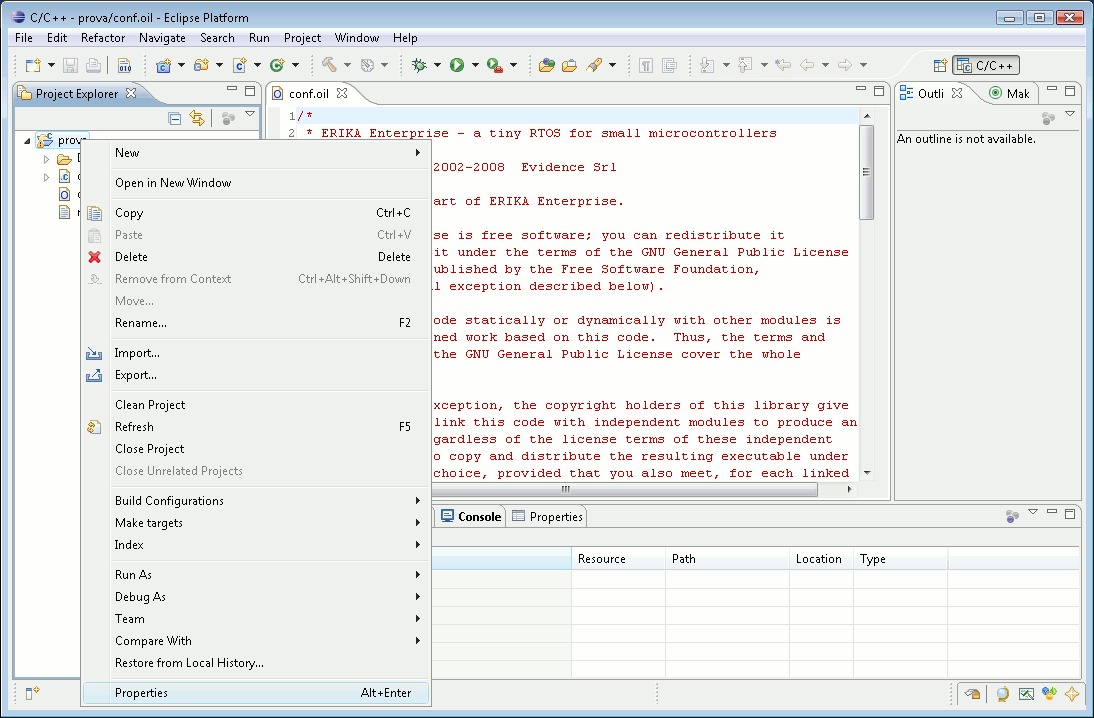
\includegraphics[width=6.3cm, bb=0 0 1094 718]{images/build1.png}
  \end{center}
  \caption{Opening the Project Properties.}
  \label{fig:build1}
\end{figure}

\begin{figure}
  \begin{center}
    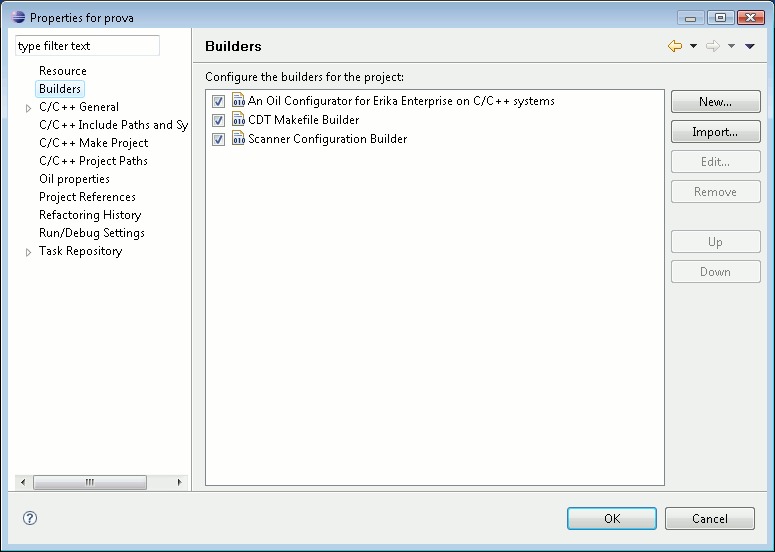
\includegraphics[width=6.3cm, bb=0 0 775 552]{images/build2.png}
  \end{center}
  \caption{The Builders property page. All checkboxes are selected by
    default.}
  \label{fig:build2}
\end{figure}

The first entry in Figure \ref{fig:build2} is relative to the \rtd\ 
Plugins shipped with Evidence, whereas the others are part of the CDT
\cite{Eclipse-CDT} plugin.




\section{Setting the OIL configuration file}

Whenever you need to set or change the OIL file that is used for code
generation, you must go to the ``Oil properties'' tab in the project
preference window. Open the Project Preference Window as shown in
Figure \ref{fig:build1}, then select the ``Oil properties'' item in
the left list, as shown in Figure \ref{fig:conf1}. After, you can type
the name of the Oil file in the ``File Name'' textbox, or you can
choose it by pressing the ``Browse'' button, as shown in Figure
\ref{fig:conf2}. The file {\em must} have a \file{.oil} extension.

\begin{figure}
  \begin{center}
    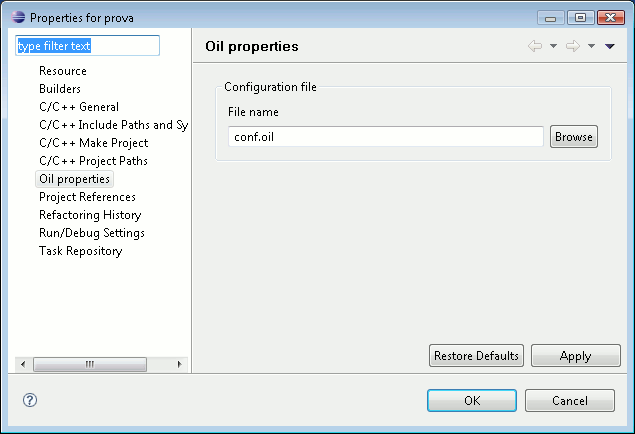
\includegraphics[width=6.2cm, bb=0 0 635 434]{images/conf1.png}
  \end{center}
  \caption{Changing the current OIL file for code generation.}
  \label{fig:conf1}
\end{figure}

\begin{figure}
  \begin{center}
    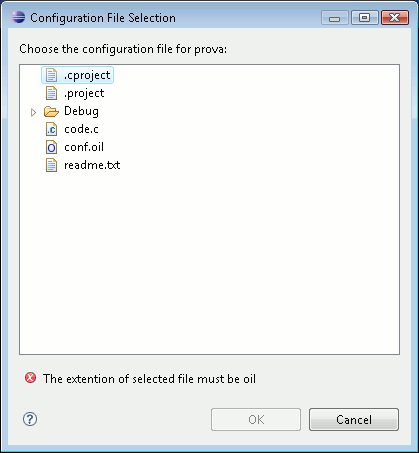
\includegraphics[width=3.5cm, bb=0 0 419 453]{images/conf2.png}
  \end{center}
  \caption{Choosing an existing OIL file by browsing the filesystem.}
  \label{fig:conf2}
\end{figure}





\section{Starting the Project Build procedure}

When the project Build is started, Eclipse executes the selected
builders. Figure \ref{fig:build2} shows the active Builders for a
project.

A project Build command can be run explicitly upon user request, or
automatically upon saving a file (see the option ``Build
Automatically'' in the ``Project'' menu). The manual execution of the
project Build command can be invoked by right clicking on the project
name in the navigation toolbar and then selecting ``Build Project'',
or directly from the ``Project'' menu, after having selected the
project in the navigation toolbar (see Figure
\ref{fig:buildproc1}).

\begin{figure}
  \begin{center}
    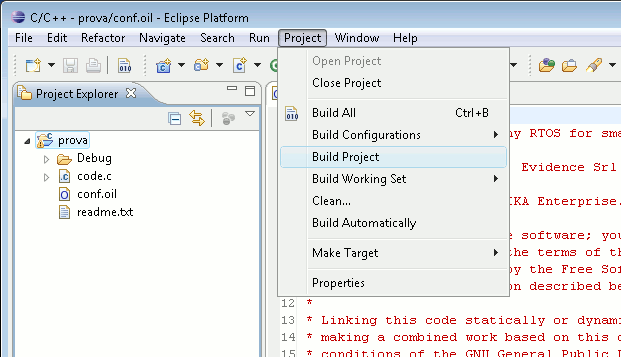
\includegraphics[width=4.4cm, bb=0 0 621 357]{images/buildproc1.png}
  \end{center}
  \caption{The ``Build Project'' option from the ``Project''
  menu. Please note that the ``Build Automatically'' option is not
  selected.}
  \label{fig:buildproc1}
\end{figure}

As a first step of the compilation process the \rtd\ builder is
launched. In this step the \rtd\ builder generates all the configuration 
scripts and the source code that is needed for the next steps of the
compilation process.

\begin{warning}
Be aware that when generating the code, the old build directories are
removed and completely overwritten!
\end{warning}

\rtd\ performs a code generation when one of the following conditions
apply:

\begin{itemize}
\item The OIL configuration file has been modified since the last
  build.
\item The Project properties have been modified, including the
  case in which the OIL configuration file name has been changed.
\item One or more files be generated do not exist anymore.
\item One or more files be generated is older than the OIL
configuration file.
\end{itemize}

The modification of the application source files does not imply
executing the \rtd\ code generation step.

The \rtd\ code generation is forced every time the OIL configuration 
file changes or the the project is cleaned as explained in Section 
\ref{project-clean}. 

After the \rtd\ builder generates the configuration source files and
scripts, the CDT builder is executed to compile the application. The
CDT Builder executes the make operation on the makefile that has been
generated by RT-Druid.

During the entire compilation phase, a progress window is displayed,
as shown in Figure \ref{fig:buildproc2}. The compilation can be done
in background by clicking on the ``Run in Background'' button in the
progress window.

\begin{figure}
  \begin{center}
    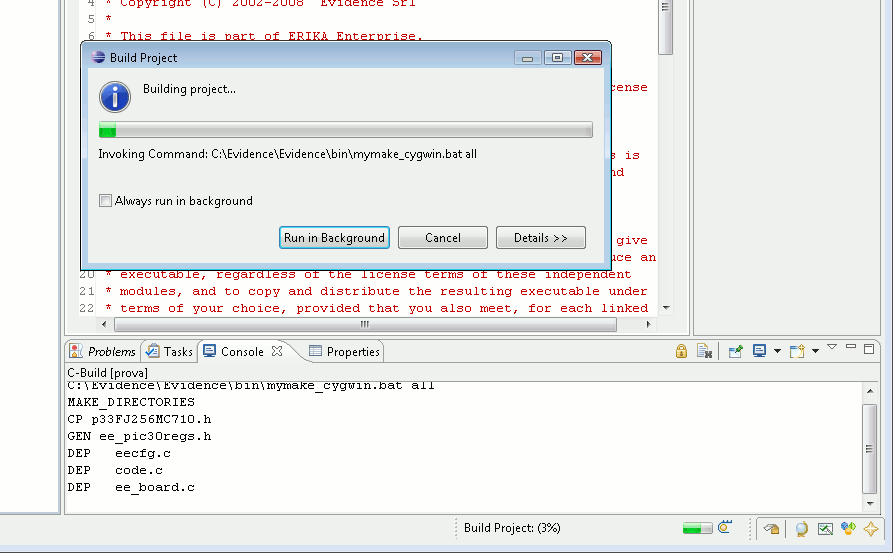
\includegraphics[width=5.1cm, bb=0 0 893 553]{images/buildproc2.png}
  \end{center}
  \caption{The Build progress window.}
  \label{fig:buildproc2}
\end{figure}

\section{RT-Druid Console}

Once the compilation process is completed, or if the compilation is
run in background, an \rtd\ console can be used to browse the messages
generated during code generation. To do that, the following steps must
be performed:

\begin{itemize}
\item Select the View ``console'' that typically appears in the 
  part of the screen after a build command.
\item Click on the monitor icon in the console view button list, and
  then choose ``RT-Druid output'' (see Figure \ref{fig:console1}).
\end{itemize}

\begin{figure}
  \begin{center}
    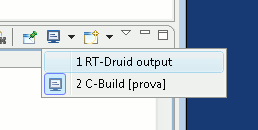
\includegraphics[width=2.3cm, bb=0 0 258 130]{images/console1.png}
  \end{center}
  \caption{Displaying the RT-Druid Console.}
  \label{fig:console1}
\end{figure}

As a result, a window like the one shown in Figure \ref{fig:console2}
appears. Please note that the text in the window can be selected and
copied as normal text.

\begin{figure}
  \begin{center}
    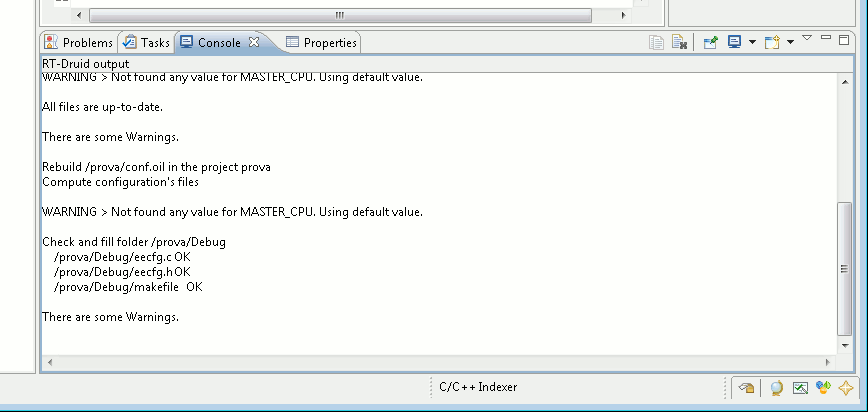
\includegraphics[width=7cm, bb=0 0 868 412]{images/console2.png}
  \end{center}
  \caption{The \rtd\ console.}
  \label{fig:console2}
\end{figure}

The pop-up menu in Figure \ref{fig:console2} can be obtained by right
clicking on the console. The menu allows to clear the content of the
console, to find strings inside it, or to drop the console\footnote{If
the console is dropped, a new one will appear at the next
build.}. Also note that upon a new build the new messages are appended
to the existing consoles.




\section{\ee\ Signatures}

The \ee\ kernel may be distributed in binary form. A so called
``binary distribution'' of \ee\ does not include the kernel C source
code, but only with a set of include files and precompiled
libraries. The \ee\ code is configured using \const{\#ifdef}
directives for efficiency reasons, and each library is the result of
the compilation of the \ee\ code with a specific combination of
\const{\#define}s.

The configurations used when generating the \ee\ libraries are
described in the \file{ee\\signature\\signature.xml} (for Altera Nios
II, the file is inside the \const{evidence_ee} SOPCBuilder component).

The location of the signature file is contained in the Eclipse
preferences, under the ``Windows/Preferences'' menu (see Figure
\ref{fig:sign1}). Then, inside the preferences Dialog box, select
``RT-Druid/Oil/OS Configurator'' (see Figure \ref{fig:sign2}).

\begin{figure}
  \begin{center}
    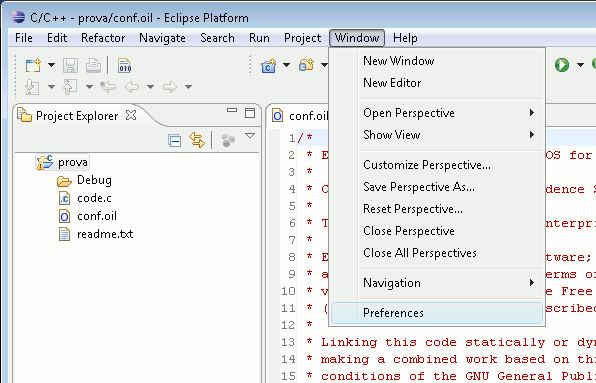
\includegraphics[width=4.6cm, bb=0 0 596 383]{images/sign1.png}
  \end{center}
  \caption{The ``Windows/Preferences'' menu item.}
  \label{fig:sign1}
\end{figure}

\begin{figure}
  \begin{center}
    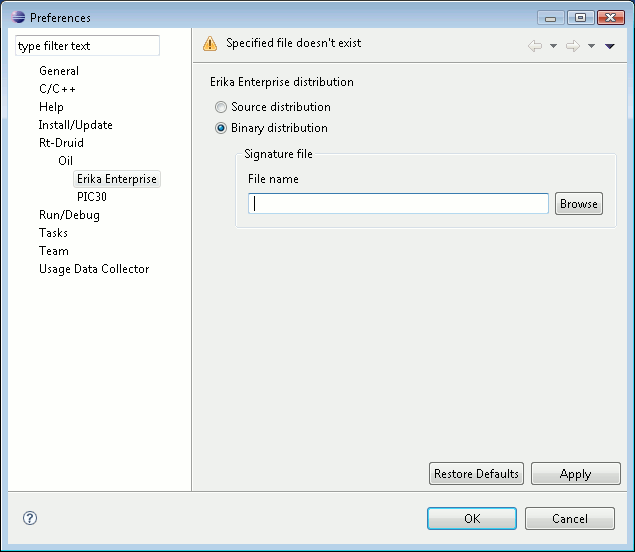
\includegraphics[width=7.3cm, bb=0 0 635 552]{images/sign2.png}
  \end{center}
  \caption{The OS Configurator dialog box.}
  \label{fig:sign2}
\end{figure}

In this box, the user can select if the code generator must be
configured for a source or for a binary distribution of \ee. When
using a Binary Distribution, the signature file location must be
specified. The standard location is ``Nios II Devices
Drivers/evidence\_ee/ee/signature/signature.xml'', as shown by Figure
\ref{fig:sign2}. Figure \ref{fig:sign4} shows the default location of
the \ee\ signatures.

If the system is correctly configured the signature file is
automatically found by \rtd\ without need of the user intervention.

\begin{figure}
  \begin{center}
    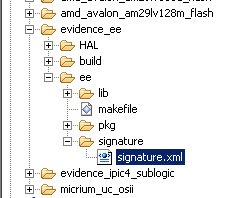
\includegraphics[width=2.4cm, bb=0 0 239 198]{images/sign4.png}
  \end{center}
  \caption{The default location of the signature file.}
  \label{fig:sign4}
\end{figure}

If \rtd\ is unable to find a library that can be used with the system
being generated, an error message is printed on the \rtd\ 
console, and the Build process is interrupted.

%\nb{(Mancano due immagini e da
%finire nel programma un mini HELP per capire come risolvere il
%problema)}

\section{Project cleanup}
\label{project-clean}

\rtd\  provides the feature to clean all the files produced by the code
generator. The cleanup process removes, if it
exists, the Build Directory.

To clean the project, just select the ``Clean...'' command inside the
``Project'' menu. The project need not be be selected if the command
is issued after selecting the project itself.

Please note the checkbox on the bottom left that can be used to build
the project right after the cleanup has been completed (see Figures
\ref{fig:clean2} and \ref{fig:clean2}).

\begin{figure}
  \begin{center}
    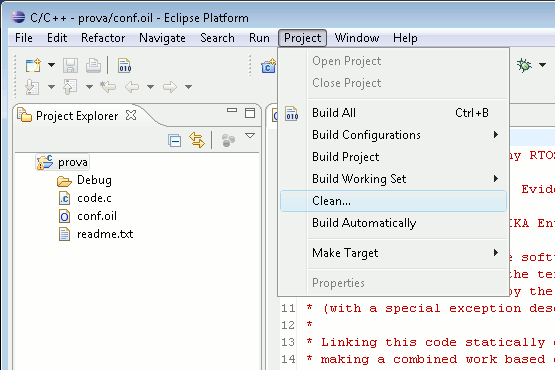
\includegraphics[width=4.4cm, bb=0 0 555 370]{images/clean1.png}
  \end{center}
  \caption{The ``Clean...'' command on the Project menu.}
  \label{fig:clean1}
\end{figure}

\begin{figure}
  \begin{center}
    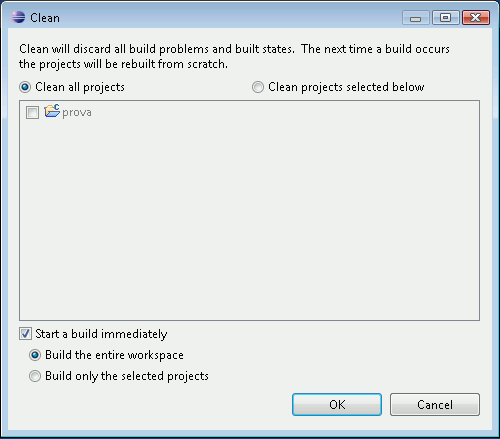
\includegraphics[width=5.3cm, bb=0 0 500 439]{images/clean2.png}
  \end{center}
  \caption{The Clean dialog box. Please note the bottom left checkbox.}
  \label{fig:clean2}
\end{figure}

Figures \ref{fig:clean3} and \ref{fig:clean4} shows the Navigation 
toolbar ``C/C++ projects'', before and after a project clean. The 
\file{Debug} directory have been removed, together with the ``Binary'' 
object list. During the cleanup, some errors may be shown in the Problem 
window. They can be ignored, since they refer to files that have been 
removed and that will be automatically re-created by \rtd\ at Build 
time. 

\begin{figure}
  \begin{center}
    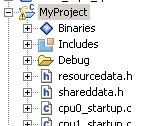
\includegraphics[width=1.6cm, bb=0 0 157 126]{images/clean3.png}
  \end{center}
  \caption{The Navigation toolbar before the Project clean.}
  \label{fig:clean3}
\end{figure}


\begin{figure}
  \begin{center}
    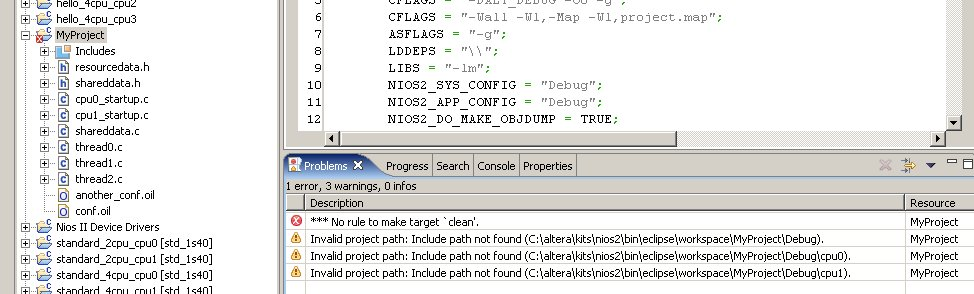
\includegraphics[width=9.8cm, bb=0 0 974 294]{images/clean4.png}
  \end{center}
  \caption{The Navigation toolbar after the Project clean. The errors
in the Problem window can be ignored, because they refer to files that
have been removed and that will be automatically created by \rtd\
at Build time.}
  \label{fig:clean4}
\end{figure}


\section{Application Debug and Run}
 
This section explicitly refers to the Altera Nios II target.

As a result of the compilation process, one ELF file for each CPU will
be placed inside the build directory. In the case of Altera Nios II,
these ELF files are equivalent to those built by traditional Altera
Build Scripts. To Debug and Run them, the best option is the creation
of a ``Multiprocessor collection'', as explained in the Altera
documentation \cite{Altera-multicpu-tutorial}.



\section{Application debug using Lauterbach Trace32}
\label{sec:trace32}

This section explicitly refers to the Altera Nios II target.

This section shows how to run a Lauterbach debug session using the
Trace32 scripts and ORTI files automatically generated by \rtd\ (see
Section \ref{sub:orti} for more information).

\begin{warning}
The scripts generated by \rtd\ suppose Lauterbach Trace32 being
installed in \file{C:\\t32}, and the Lauterbach ORTI utility
\file{genmenu.exe} being installed insie
\file{C:\\T32\\demo\\kernel\\orti}.
\end{warning}

Once the application has been compiled, and the Trace32 scripts have
been generated, launch Trace32 by double clicking on the
\file{Debug/debug.bat} file generated during the compilation. The
debugger opens up showing a window similar to the one in Figure
\ref{fig:trace32_splash}.

%
\begin{figure}
\begin{center}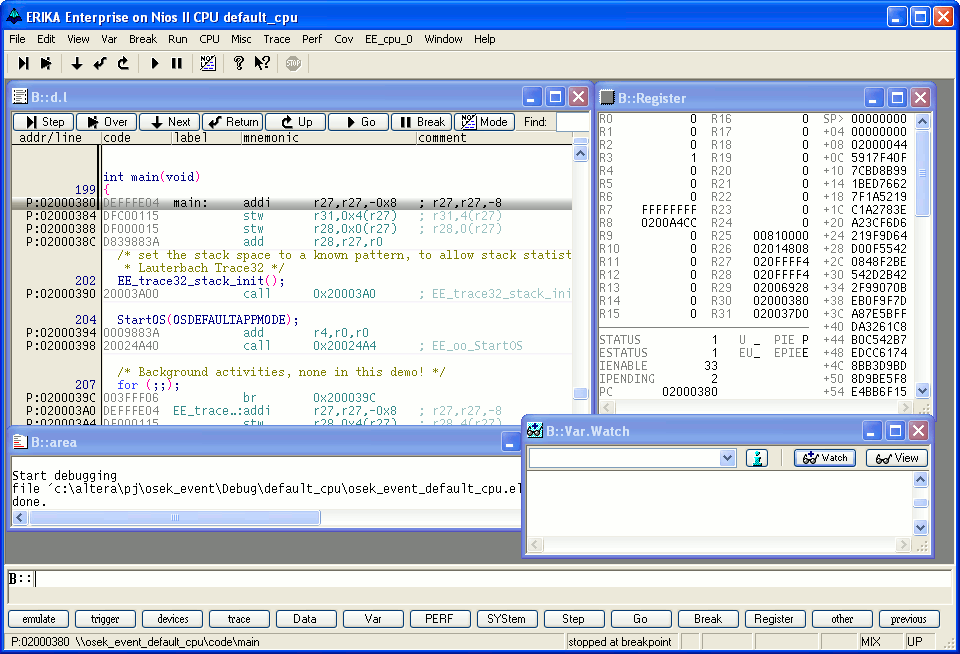
\includegraphics[%
  width=12cm, bb=0 0 960 654]{images/trace32_splash.png}\end{center}
\caption{\label{fig:trace32_splash} The Lauterbach Trace32 for Altera
Nios II.}
\end{figure}
%

Please note that each window has a title
with the name of the CPU being under debug. The menu list include a
submenu named ``ee\_cpu\_0'' containing the specification of the ORTI
related debug features.

By clicking on each menu item, you can get useful debug informations
about \ee. In particular:
\begin{itemize}
\item Figure \ref{fig:trace32_os} shows the general information about
  the kernel global variables, such as the name of the running task,
  the current priority of the running task, the last RTOS primitive
  called, the last error returned by an \ee\ primitive, the current
  application mode and the current system ceiling.
%
\begin{figure}
\begin{center}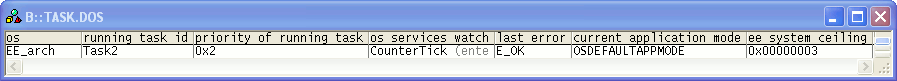
\includegraphics[%
  width=12cm, bb=0 0 897 81]{images/trace32_os.png}\end{center}
\caption{\label{fig:trace32_os} General information about the \ee\ status.}
\end{figure}
%

\item Figure \ref{fig:trace32_task} shows, for each task, the task
  name, its current priority, which may be different from the nominal
  priority when the task lock a resource, the task state, the task
  stack, and the current pending activations.
%
\begin{figure}
\begin{center}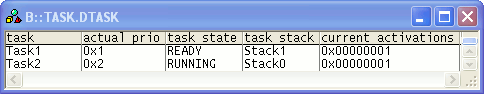
\includegraphics[%
  width=11cm, bb=0 0 484 94]{images/trace32_task.png}\end{center}
\caption{\label{fig:trace32_task} Information about the tasks in the
system.}
\end{figure}
%

\item Figure \ref{fig:trace32_resource} shows, for each resource, the
  resource name, the resource status, the task that has locked the
  resource (if any), and the ceiling priority of the resource.
%
\begin{figure}
\begin{center}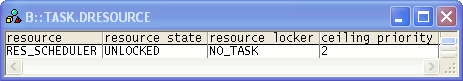
\includegraphics[%
  width=9cm, bb=0 0 463 81]{images/trace32_resource.png}\end{center}
\caption{\label{fig:trace32_resource} Information about the resources
in the system.}
\end{figure}
%

\item Figure \ref{fig:trace32_alarm} shows, for each alarm in the
  system, the alarm name, the time to which the alarm will fire, the
  cycle time of the alarm (\const{0x0} means the alarm is not cyclic),
  the alarm state, the action linked to the alarm notification, the
  counter to which the alarm is attached, and its value.
%
\begin{figure}
\begin{center}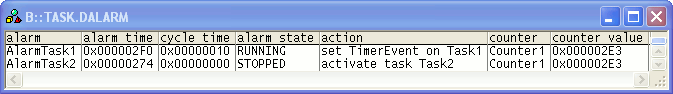
\includegraphics[%
  width=11cm, bb=0 0 673 94]{images/trace32_alarm.png}\end{center}
\caption{\label{fig:trace32_alarm} Information about the alarms in the
system.}
\end{figure}
%

\item Finally, Figure \ref{fig:trace32_stack} and Figure
  \ref{fig:trace32_stackview} show information about the stacks that
  has been configured in the application. In particular, the first
  figure shows the stack name, size, base address, direction, and fill
  pattern, while the second figure shows in a graphical way the
  current stack usage. To obtain the graphical stack usage estimation
  the application has to call \fn{EE_trace32_stack_init} at system
  startup. In this example, \const{Stack0} is the shared stack used by
  the background task (the \fn{main} function), and by
  \fn{Task2}. \fn{Stack1} is used by \fn{Task1}, and \fn{Stack2} is
  the interrupt stack.
%
\begin{figure}
\begin{center}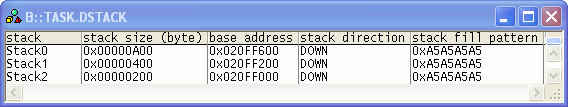
\includegraphics[%
  width=11cm, bb=0 0 568 107]{images/trace32_stack.png}\end{center}
\caption{\label{fig:trace32_stack} The application stack list.}
\end{figure}
%
\begin{figure}
\begin{center}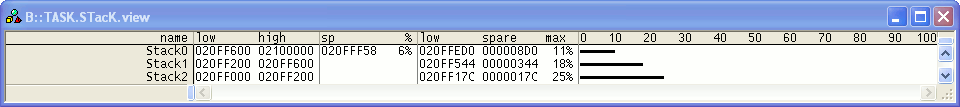
\includegraphics[%
  width=13cm, bb=0 0 960 107]{images/trace32_stackview.png}\end{center}
\caption{\label{fig:trace32_stackview} A graphical view of the
application stack usage.}
\end{figure}

\end{itemize}


The \rtd\ and \ee\ Trace32 support also includes support for the Nios
II tracer module. As an example, Figure \ref{fig:trace32_chart_irq}
shows the execution of an interrupt handler as recorded by the tracer
module. Figure \ref{fig:trace32_chart_state} shows an interpretation
of the context changes and task status values using the ORTI
information.

%
\begin{figure}
\begin{center}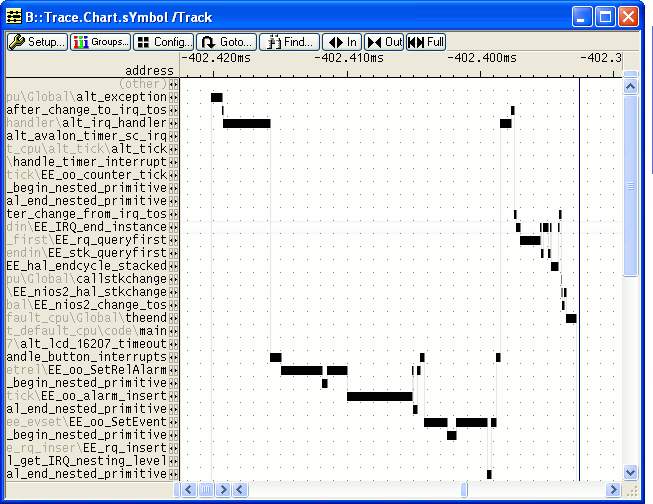
\includegraphics[%
  width=11cm, bb=0 0 653 504]{images/trace32_chart_irq.png}\end{center}
\caption{\label{fig:trace32_chart_irq} The execution of the Button IRQ
as recorded by Lauterbach Trace32.}
\end{figure}

%
\begin{figure}
\begin{center}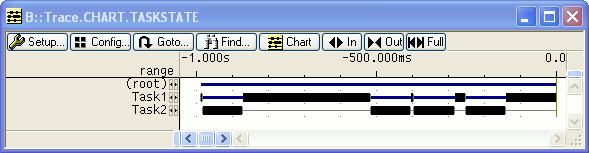
\includegraphics[%
  width=11cm, bb=0 0 589 153]{images/trace32_chart_state.png}\end{center}
\caption{\label{fig:trace32_chart_state} The interpretation of a trace
recorded with Lauterbach Trace32 showing the context changes happened
in the system.}
\end{figure}

\subsubsection{Acknowledgements}

We would like to thank Ing. Maurizio Menegotto from Lauterbach Italy
Srl for his support in the integration of \rtd\ and \ee\ with the
Lauterbach Trace32 Debugger and Tracer.


\chapter{Standalone version of \rtd}
\label{cha:Commandline}

\section{Introduction}

This chapter describes the standalone version of \rtd. The idea behind
of the standalone version is to provide the \rtd\ code generator
plugin packed {\em without} the Eclipse Framework, to have a simple and
fast way to generate code and templates from the command line.

The standalone version of \rtd\ is stored inside the \file{bin}
directory inside the \rtd\ installation directory.

\section{Code generation}
To generate code using the standalone version of \rtd, please run the
following command:

\begin{lstlisting}
rtdruid_launcher.bat --oil filename --output dir
\end{lstlisting}

\noindent Where:
\begin{itemize}
\item \const{filename} is the name of the OIL file.
\item \const{dir} is the directory where the generator should put the
  generated files. The \const{--output} option is optional. If not
  specified, the default directory name used is \const{Debug}.
\end{itemize}

\section{Template code instantiation}
This section explains how to obtain the automatic generation of a
template example, as it is done from the ``New Project'' menu item
from the Eclipse Framework.

To obtain the list of available templates, please run the following
command:

\begin{lstlisting}
template.bat --list
\end{lstlisting}

\noindent as a result, the command displays a list of the available
templates, with their IDs.

Then, to instantiate a template, please run the following command:

\begin{lstlisting}
template.bat --template ID --output dir
\end{lstlisting}

\noindent Where:
\begin{itemize}
\item \const{ID} is one of the IDs returned using the \const{--list} command..
\item \const{dir} is the directory where the generator should put the
  generated files. The \const{--output} option is optional. If not
  specified, the default directory name used is the current directory.
\end{itemize}


\part{Schedulability Analysis Plugins}
\chapter{Schedulability Analysis Plugins Introduction}
\label{cha:schedulability-analysis-introduction}

\section{Generalities}


\subsection{Background}

Embedded control systems development is about producing systems or
sub-systems according to a set of specifications dictating their
required (physics) properties. The output of the design stage is a set
of models that describe the system at different levels of
abstraction. Properties and constraints are captured by mathematical
formalisms.

A typical design flow of embedded software (a v-shape process is
represented in Figure~\ref{fig:V-shaped-design-process.}) includes
(among others) two stages of fundamental importance. The first stage,
at the logical level, is the domain of application developers such as
control engineers or other domain experts and produces a model of the
software application providing a solution to the functional
requirements in terms of one or more block diagrams. Most commercial
design flows provide extensive support for this stage. Compliance
against functional requirements is typically validated by extensive
simulation and the risk of functional errors due to incorrect
implementation is reduced by tools for the automated translation of
the model (Real-Time Workshop Embedded Coder or TargetLink).

%
\begin{figure}
  \begin{center}
    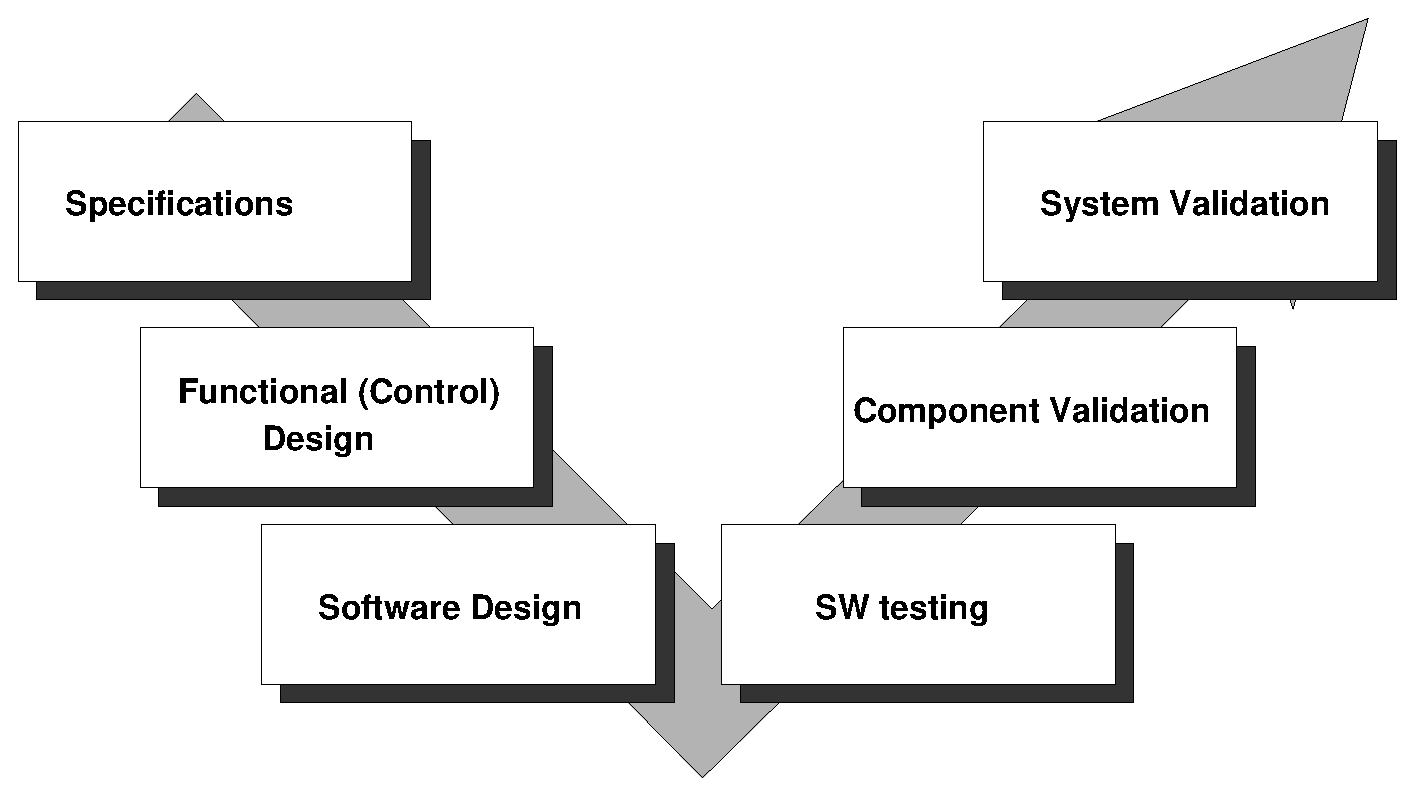
\includegraphics[width=10cm]{images/vshape}
  \end{center}
  \caption{V-shaped design process.}
  \label{fig:V-shaped-design-process.}
\end{figure}


The second stage of the design process is at the architecture level,
where software engineers (real-time systems experts) map the
functions/components developed in the previous stage to real-time
threads, select the scheduler and the resource managers by exploiting
the services of a Real-Time Operating System (RTOS) and ultimately
check the correctness of the timing requirements upon the target (HW)
architecture. This design stage is transparent to software
functionality (only provides its implementation), but it is crucial to
achieve performance/cost trade-offs with the objective of providing
the best possible quality and the best possible accuracy to system
functions within the timing constraints and/or the performance target.


\subsection{Problem description}

Unfortunately, even in state-of-the-art processes, the above steps are
performed relying solely on the skills or the experience of project
developers. As a consequence, projects often suffer from design errors
that show up only after deployment with obvious economic losses. If
the software manufacturer detects timing errors or unsatisfactory
performance during the extensive testing period, a chain of
engineering changes is initiated that implies many iterations between
the logical and the architectural view, trading implementation
complexity for schedulability (or time performance) and tuning many
design parameters, including system resources and (when possible)
activation rates.

The separation of the design environments for functionality and for
time, together with the limited support (feedback) provided by the
existing tools make the process quite inefficient. Trial-and-error
iterations are often performed without a clear knowledge of what
should be modified and how.


\subsection{Innovating the architecture design}

Schedulability analysis theory bears the promise to fill in this gap,
since it enables formal validation of the timing behavior of
architecture-level solutions at the highest possible level in the
flow. To this purpose, timing properties and constraints should be
explicitly stated (by appropriate design annotations) and the
(hardware and software) resources available for the execution of the
application tasks and the resource allocation and scheduling policies
must be clearly stated in appropriate design environments.

We take inspiration from recent literature in the field of embedded
systems design, where a clear separation of concerns between
functional design and implementation choices is advocated and the use
of a shared set of abstractions allows for an efficient exchange of
information between the two activities. In this way, the functional
design remains independent from architectural choices and it does not
require an advance commitment to any specific implementation.


\section{The envisioned methodology: Architecture-level design}
\label{sec:envisioned-methodology}

\subsection{Introduction }

The distinctive aspect of schedulability analysis is a match between
the timing (or, in general, QoS) requirements of logical entities in
the logical layer and the corresponding QoS offers of an
implementation or architecture layer (Figure
\ref{fig:logical-phisical}) and consequently raises the fundamental
problem of mapping logical-level entities into architecture-level
entities \cite{OMG-PST02}.

The logical architecture\footnote{In the sequel, we shall use the
  adjective s{}``logical'' and {}``functional'' interchangeably.} (or
functional model) consists of a network of functional blocks or
components connected by means of communication variables and it is the
outcome of the control design phase. This network is typically a
straightforward derivation of the control schemes produced, for
example, using such CAD tools as Matlab/Simulink or ETAS ASCET-SD.
The concurrency description layer contains an implementation
description consisting of all the threads that are running in the
system and of the policies for managing resources (possibly
implemented in the operating system). Finally, the hardware layer
describes the hardware and its QoS features. The two bottom layers
collectively define the so-called physical architecture layer,
describing the mapping of the functional or logical design to a
particular real-time execution environment.

\begin{figure}
  \begin{center}
    \includegraphics[width=8cm]{images/logical-phisical.eps}
  \end{center}
  \caption{Schedulability analysis requires creating a correspondence
    between logical and physical architecture.}
  \label{fig:logical-phisical}
\end{figure}


The mapping stage consists of assigning each functional block to a
software thread and each communication variable to a communication
facility of the implementation (e.g. a task's private variable, a
protected shared variable, etc.). It also includes an appropriate
choice for such high level execution parameters as task activation
rates. In order to comply with the timing constraints, it is crucial
to perform appropriate choices for such real-time scheduling
parameters as, at this stage, task priorities and ceilings for
semaphores protecting shared resource (see the OSEK/VDX
specification). To this regard, a fundamental aid is offered by
schedulability analysis. This activity is performed right after
mapping (Figure \ref{fig:Schedulability-analysis}) to test the
correctness of a mapping hypotheses and to automatically synthesize
some of the real-time scheduling parameters.


\begin{figure}
\begin{center}
\includegraphics[width=10cm]{images/flow}
\par\end{center}
\caption{\label{fig:Schedulability-analysis}Schedulability analysis in
  the design flow}
\end{figure}


Several mapping-schedulability analysis iterations can be required
before coming up with a satisfactory design. In our envisioned
methodology such iterations are not \emph{blind-eyed} since
schedulability analysis does not simply provide a boolean answer on
the schedulability of the system, but it returns performance
information (i.e. response times) and sensitivity analysis. This
feedback drives mapping and/or architecture design changes but it can
also provide a measure of the resource (time) budgets that should be
accounted for in a possible functional redesign stage.


\subsection{Logical level design }
\label{sub:Logical-level-design}

At the logical level, most real-time systems feature a control and a
dataflow part. The dataflow part is often time-driven, since inputs
are sampled at regular intervals and it is suitable for an
implementation consisting mainly of periodic activities. In contrast,
the control-dominated functionality is highly asynchronous
(event-driven) and state-dependent.

The model of the system represents both parts with suitable
abstractions.  The syntax and the semantics of the modeling language
used by control engineers may vary, but in general, all models provide
a meta-representation of the design as a structure or network of
(functional) components connected via nets to each other's ports
(mechanisms to communicate between blocks, such as shared variables)
and communicating with each other using message (event)
abstractions. Messages may be asynchronous (signals) or synchronous
(call messages).

We provide a very simple and general metamodel (and a corresponding
syntax based on XML) for representing an abstraction of the functional
model where each component and event is annotated with timing
attributes and constraints, such as assumptions on the maximum rate of
arrival of events and on the worst case computation time of
components. This abstraction is suitable for specification of
architecture-level mapping and verification of timing properties.


\subsection{Software architecture design }
\label{sub:Software-architecture-design}

If the logical architecture primarily focuses on functional
requirements, the physical architecture level is where physical
concurrency, resource requirements and schedulability constraints are
expressed. At this level, the units of computation are the processes
or threads (or in general, tasks), executing concurrently in response
to environment stimuli or prompted by an internal clock. Tasks
cooperate by exchanging data and synchronization or activation signals
and compete for the use of shared resources (including the processor,
shared buffers, network links, etc.). Eventually, all logical entities
have to be mapped onto corresponding software architectural entities,
and the latter have to be mapped onto target hardware components in
the physical architecture level. This activity entails the selection
of an appropriate scheduling policy (for example, offered by a
real-time operating system), which must be clearly supported by
techniques for analyzing schedulability.

Our conceptual model uses the concepts of execution engine, scheduling
policy, resources, and schedulable resources to model the elements
of a physical architecture. An execution engine models the processing
resource and has a scheduling policy that determines how the tasks
will be scheduled. 


\subsection{Mapping}
\label{sub:Mapping}

The mapping process consists of establishing an \emph{implemented by}
or realization relationship between functional components and
architecture-level objects (such as tasks) and in the definition of a
binding or deployment relationship between threads and resources and
hardware components. The mapping relationship is constrained by the
specifications defined at both the logical and the architecture
levels, such as precedence and exclusion constraints among functional
blocks or timing constraints enforcing the activation rates of
software actions.

Mapping and binding decisions have crucial impact on the result of
timing analysis. Load balancing and local schedulability clearly
depend on binding decisions, when multiprocessor architectures are
considered.


\subsection{Schedulability Analysis}
\label{sub:Schedulability-Analysis}

Once the application functional model has been mapped on to a set of
real-time tasks, it is necessary to verify that all temporal
constraints are respected before actually implementing the system.

A real-time task is characterized by a period T (or minimum
interarrival time or maximum activation rate), by a relative deadline
D (i.e. the time computed from the activation by which each job must
complete) and by a worst-case execution time C. The goal of the
schedulability analysis is to check if all jobs can execute C units of
execution time between their activation time and their deadline.

For example, all OSEK-compliant OS provide the fixed priority
scheduling algorithm. For the fixed priority scheduling algorithm,
three different schedulability analysis can be performed: the
utilization-based test, the response time test and the hyperplane
test.

In case of detected timing failures, the Schedulability Analysis
returns feedback to the mapping in a form that allows the designer to
pinpoint the exact cause that lead to schedulability or timing errors
and give a range of actions as well as a measure of the entity of the
corrections that would make the design feasible.


\section{The Schedulability Analysis plugins}

The Schedulability Analysis plugins of \rtd\ aids the designer in
modeling, analyzing, and simulating the timing behavior of embedded
real-time systems. Being an open and extensible environment based on
XML and open standards (Java), \rtd\ can be easily integrated with
existing systems.

\begin{figure}
\begin{center}
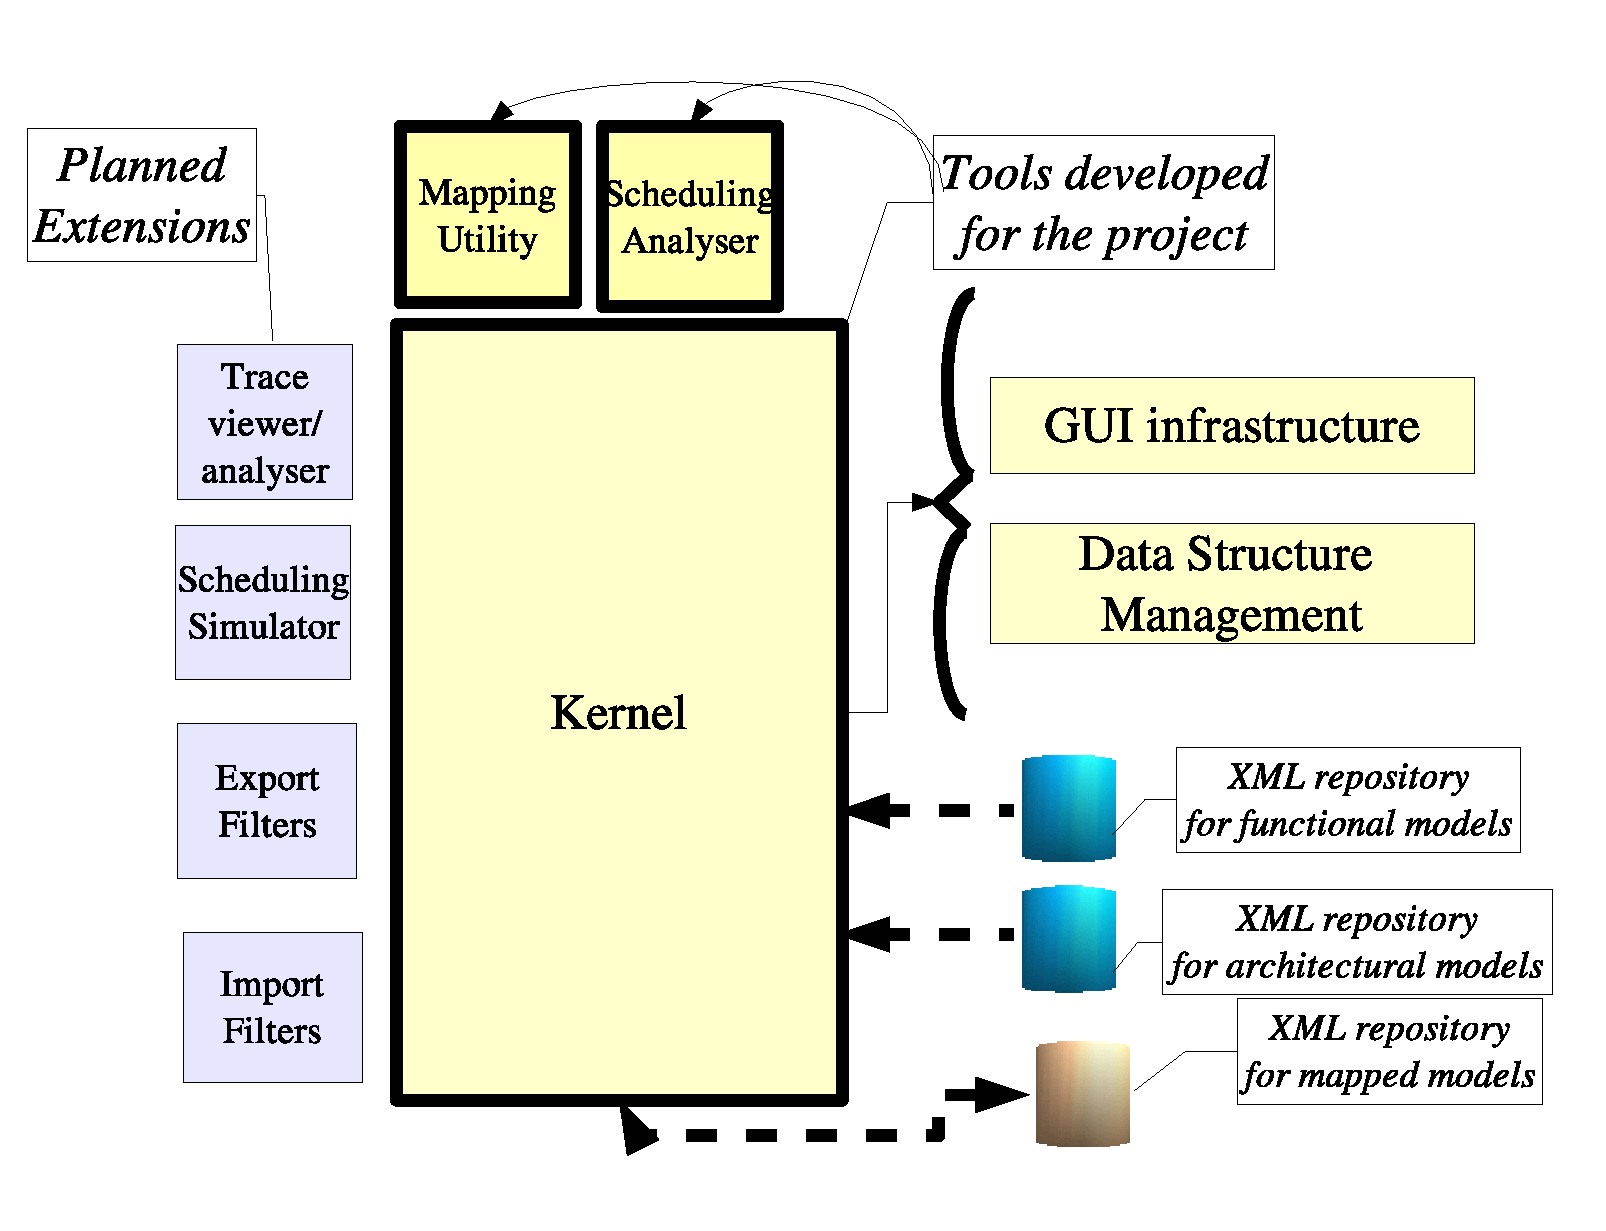
\includegraphics[width=10cm]{images/architecture}
\end{center}
\caption{\rtd\ architecture}
\label{fig:RTDruid-architecture}
\end{figure}


The \rtd\ schedulability plugins have a modular architecture shown in
Figure \ref{fig:RTDruid-architecture}.  Model information (i.e. for
both the functional and the architecture-level parts) is stored in an
internal repository and it is made available by means of an open
format based on XML. The tool set architecture is based on a kernel
module, providing management of internal data structure and basic
services for GUI and additional plugin modules.  Plugins exploit
kernel services in order to provide support to the design stages in a
completely independent way.

The modeling and mapping module provides general Graphics and Text
Diagrams to capture textual requirements, flowcharts, component and
deployment notation and other general purpose information. Design
teams can develop a representation of the embedded real-time system in
graphical or textual form and capture the interaction between
functional and architecture-level designs without disrupting the
existing development process. This is done by using a neutral
(XML-based) format and metamodel.  Both logical and architecture-level
modeling entities can be interactively defined within the context of
the tool or imported by translation from external models. XML-based
import/export utilities enable the transfer of information between our
tools and other tools supporting XML or text-based standards. Modeling
elements for logical and architecture-level abstractions mirror the
definitions given in the previous sections.

The \textbf{schedulability analyzer} plugin provides support for worst
case timing analysis. The module interacts with the other components
by exchanging design information in the form of back annotations
according to the schema of Figure
\ref{fig:schedulability-analysis-interactions}. The forward path of
Figure \ref{fig:schedulability-analysis-interactions} represents the
communication of the system model (as defined in the previous
sections) to the schedulability analysis tool. The inverse model
conversion provides an alternate option for using the results of the
schedulability analysis since it can produce its results in the same
XML files that are used to encode the design information. In
particular, it stores the values for the attributes (priority,
priority ceiling) that are synthesized based on the selected
scheduling policy and the schedulability results
themselves. Back-annotating the results into the same XML file that
represents the model of the system helps the designer in keeping all
the information related to the current iteration in the design flow
aligned and consistent.

\begin{figure}
\begin{center}
\includegraphics[width=10cm]{images/interoperability}
\end{center}
\caption{Interactions between the kernel module and the Schedulability analyzer.}
\label{fig:schedulability-analysis-interactions}
\end{figure}

% These are not implemented yet
%The \textbf{trace viewer/analyzer} provides support for estimating the
%execution time attributes of software components

%The \textbf{Scheduling simulator} enables an evaluation of the worst
%case response time of the threads needs to be supplemented by simulations
%of average as well as critical runs highlighting the expected time
%behavior of the system. 

%The \textbf{Export/import} filters automatically imports model diagrams
%from existing tools such as Simulink, ASCET or UML-based design frameworks. 

%The \textbf{Automatic code generation} features automates the production
%of functional as well as architecture-level code and debugging information
%in OSEK-compliant systems.


\subsection{Status of the Schedulability analysys plugin}

As shown in Figure \ref{fig:RTDruid-architecture}, the current version
of the tool offers a set of components that enables the user to
perform a schedulability analysis of the system under design. A
graphical GUI based on the Eclipse Project is available, which allows
the user to edit the input files, perform the schedulability analysis
and to visualize the related results.

The tool can be used as follows (see Figure \ref{fig:RTDflow}):

\begin{figure}
  \begin{center}
    \includegraphics[width=6.3cm]{images/RTDruid_flow3.eps}
  \end{center}
  \caption{Status of the Schedulability analysis plugin.}
  \label{fig:RTDflow}
\end{figure}

\begin{itemize}
\item The user is required to specify the system (inclusive of
  functional model, software architecture and mapping) by means of XML
  files, whose format is documented in Chapter
  \ref{cha:DTD-Input-file}. The input files can be edited with any
  text editor, or with the GUI. The system specification can be
  contained in one single XML files, or it can be split among many
  files. The tool will automatically merge all files in one single
  specification. The initial specification may also come from an input
  file expressed in OSEK OIL or AUTOSAR XML (typically in these cases
  the model must be augmented with execution time informations since
  these file formats are not meant for schedulability analysis but
  only for RTOS configuration).
\item Once the system has been specified, the user can run the tool in
  either batch mode or in graphical mode. To perform the operations in
  batch mode, the user must provide a Ant script file (see the Apache
  Ant project on the Apache web site). The script file features are
  described in Chapter \ref{cha:Script-File}. The tool invocation
  results into the execution of commands specified in the script file.
\item The results of schedulability analysis are then reported in an
  output file as well as in the \rtd\ Table view (if run from the
  graphical interface). It is possible to annotate the results in the
  same input files in a specific section.
\end{itemize}


\chapter{Format of the Input File}
\label{cha:DTD-Input-file}


\section{Introduction}

This chapter describes the structure and the syntax of the RTD XML
format, which is used to describe the main component of a system. The
RTD format has been used since the first versions of \rtd\ as the
source of the information for the schedulability analysis plugin.

The DTD of the RTD specification is contained in the file
\file{templates/evidence.DTD} of the \rtd\ documentation.
% FIXME: check if the file position is still correct.

The structure of this chapter is the following: first, it describes
the development process of an embedded real-time system with \rtd, and
how the different steps of this process are reflected in the sections
of the \rtd\ input file. Then, it details the structure of the DTD,
describing each of its sections with examples. Finally, it describes
other miscellaneous, like common elements and conventions.


\section{Development process with \rtd}

The objective of the \rtd\ schedulability plugins is to help the
system designer in all phases of the design and development of a
complex embedded application. For this reason, the input file is
divided into different sections, each one containing information on a
single phase of the design and development process. In particular, we
envision the following steps:
\begin{itemize}
\item Modeling the functional behavior of the application. In this
  phase, the designer models the behavior of the system and of the
  application without any regard to the implementation of the system
  on a specific platform. This phase is typically done with tools like
  Matlab/Simulink, or similar. The description of the functional model
  of the system is done in the \const{FUNCTIONAL} section of the input
  file (see Section \ref{sec:Functional-section} for details).
\item Modeling the software and hardware architecture of the
  system. In this phase, the designer models the characteristics of
  the platform on which the application will be implemented. This
  involves the definition of the number of computational nodes, the
  number and types of processors for each node, the RTOS used on each
  node, the number of real-time tasks, etc. The architectural model is
  specified in the \const{ARCHITECTURAL} part of the \rtd\ input file
  (see Section \ref{sec:Architectural-section} for more details).
\item Mapping the functional model to the architectural model. In this
  phase, the functional elements defined in the \const{FUNCTIONAL}
  section are ``mapped'' on to the appropriate architectural
  elements. For example, it is important to decide which task will
  perform a specific operation of the applications, and on which
  node/RTOS such task is allocated. Of course, many different mapping
  choices are possible, and the choice of the mapping can influence
  the performance of the system. In the \rtd\ input file, the mapping
  is specified in the \const{MAPPING} section (see Section
  \ref{sec:Mapping-section} for more details).
\item Back-annotation of performance measurement. In this phase, the
  system is run under specific testing conditions, and the performance
  of each element is measured and back-annotated. For example, in this
  phase each task is run under different conditions and the execution
  time is measured and recorded. At the end of the test, the
  average-case and worst case execution time of the task can be
  obtained. These information will be useful for the next phase, the
  schedulability analysis. The back-annotation information is
  contained in the \const{ANNOTATION} section of the \rtd\ input file
  (see Section \ref{sec:Annotation-section} for more details).
\item Schedulability analysis. In this phase, a systematic off-line
  analysis of the system is performed. The analysis will tell the
  designer if the system is schedulable (i.e. if all tasks will
  complete in time) under all conditions. Moreover, the analysis gives
  back additional sensitivity information about the system. For
  example, if the system is not schedulable, the analysis tells us
  which task will miss its deadline and how it is possible to modify
  the system the avoid this.  In case the system is schedulable, it
  tells us how much ``free space'' is left before a deadline is
  missed. The results of the analysis are provided by the tool in the
  \const{SCHEDULABILITY} section (see
  Section\ref{sec:Schedulability-section} for more details).
\end{itemize}

Not all sections are mandatory. In most cases, it is possible to
specify only some section and still be able to analyze the system. For
example, under certain conditions, the \const{FUNCTIONAL} section need
not to be specified. This is useful, for example, when analyzing
systems that are already implemented.


\section{RTD and ERTD files}

The \rtd\ schedulability plugin stores the input files in two
different formats, each one having a different file extension, as
shown in Table \ref{tab:file-formats}.

%
\begin{table}
\begin{centering}
\begin{tabular}{|c|p{7cm}|}
\hline 
File extension & Description
\tabularnewline
\hline
\hline 
.RTD & XML file format that has been created for ease human processing.
\tabularnewline
\hline 
.ERTD & XML file format automatically generated by EMF. That format is not
suited for readability. 
\tabularnewline
\hline
\end{tabular}
\par\end{centering}

\caption{XML file formats used by the \rtd\ Tool set.}
\label{tab:file-formats}
\end{table}


The two formats express the system semantic in a different form: the
.ERTD form is suited for automatic processing by the EMF automatically
generated loader, whereas the .RTD form is more easily readable, and
hence it is more suited for manual editing. This chapter only
describes the .RTD style XML file structure. The .ERTD file structure
is an internal XML representationand and it is not described in this
manual.

\textbf{Note:} \rtd\ uses the file extension to discriminate which
file format should be expected as content. Files in .RTD form are
parsed by an XSLT sheet, converted in .ERTD form, and then loaded.
When saving the file from the GUI it is possible to save in both formats.


\section{.RTD XML file structure}

The purpose of the file format presented in this section is to describe
all the aspects of a complex system. As its root, a system is composed
by a single \const{system} element, that contains a \const{Name}
attribute used to discriminate between different instances of systems.
The following is an example of a system definition:

\begin{lstlisting}
<?xml version="1.0" encoding="UTF-8"?>
<SYSTEM Name="mySystem">
[...]
</SYSTEM>
\end{lstlisting}

Each system is described using sections. Each section is used to
describe a particular phase of the design methodology that
\rtd\ proposes.  Here is a quick list of the various sections that
compose a system description:

\begin{description}
\item [{modes}] The modes section is used to list different working
  modes of a system. See section \ref{sec:Mode-section}.
\item [{functional}] The functional section contains all the elements
  that describe the functional part of the system. The functional part
  of a system is in general composed by different elements, named
  \const{PROC}, \const{VAR}, \const{SUBSYSTEM}, and \const{TRIGGER}
  (external events).  Moreover, the functional part contains the
  \emph{use} relationships between the different elements in the
  system, the \emph{partial ordering} between different events
  (start/end of a method, proc activation, trigger arrival). For each
  element it is possible to specify some temporal characterization,
  such as periodicity, deadline, minimum interarrival time, jitter and
  offset (see sections \ref{sub:Logical-level-design} 
  % FIXME reference not found
  and \ref{sec:Functional-section}).
\item [{architectural}] The architectural section contains the
  specification of different parts of the system that are of interest
  for the purpose of mapping. This section contains, for example,
  elements such as \const{ECU}, \const{CPU}, \const{TASK},
  \const{SEMAPHORE}s, \const{BUS} and related \const{FRAME}s. This
  section does not contain the relation between tasks and CPUs, that
  is instead contained in the mapping section.  If a system includes
  only the architectural but not the functional section, all the
  references to \const{VAR}s are substituted with resources that
  otherwise are ignored (see Sections
  \ref{sub:Software-architecture-design} 
  % FIXME reference not found
  and
  \ref{sec:Architectural-section}).

\item [{mapping}] The mapping section is used to describe the
  assignment of \const{PROC}s to \const{TASK}s, to specify which RTOS
  a task is assigned to, and to specify if a \const{VAR} element
  should be implemented as a mutex or through a bus frame. These
  information depend on the system application modes (see sections
  \ref{sub:Mapping} 
  % FIXME ref not found
  and \ref{sec:Mapping-section}).
\item [{annotation}] The annotation section includes the temporal
  information related to the execution times of each task and of each
  method related to proc, var and resources. This information depends
  on the system application modes (see section
  \ref{sec:Annotation-section}).
\item [{schedulability}] The schedulability section contains the
  result of the schedulability test that is made for each CPU and for
  each task. This information depends on the system application modes
  (see sections \ref{sub:Schedulability-Analysis} and
  \ref{sec:Schedulability-section}).
  % FIXME ref not found
\end{description}

It is not possible to describe more than one system inside a single
input file. Not all the sections just described are mandatory in an
instance of an input file, however it must be clear that some features
may be disabled in case of missing informations. For example,
schedulability tests cannot be performed if computation times are
missing.

All the identifiers in an input file are \emph{case insensitive},
except for the references that must contain the exact name of an
object (that usually has a one-to-one relation with some identifier
used in the source code).


\paragraph{Example}

Here is an example of a typical XML file structure.

\begin{lstlisting}
<?xml version="1.0" encoding="UTF-8"?>
<SYSTEM Name="...">
  <MODES>
    [...]
  </MODES>
  <FUNCTIONAL>
    [...]
  </FUNCTIONAL>
  <ARCHITECTURAL>
    [...]
  </ARCHITECTURAL>
  <MAPPING>
    [...]
  </MAPPING>
  <ANNOTATION>
    [...]
  </ANNOTATION>
  <SCHEDULABILITY>
    [...]
  </SCHEDULABILITY>
</SYSTEM>
\end{lstlisting}

The following sections present in detail the content of each section
in the XML file, detailing all the elements that characterize each
part.


\section{Mode section}
\label{sec:Mode-section}

Modes are abstractions that can be used to specify a configuration of
the system that is used only under particular working conditions.  For
example, an airplane controller probably has different control
algorithms when the airplane is taking off, flying and landing, and
these algorithms have requirements expressed by a different set of
tasks, resources, and so on. For this reason, the specification of
modes in the system is useful for describing the behavior and the
composition of the system in all its aspects and in an unified way.

Modes typically influence the mapping phase, because it is in that
phase that the designer decides:

\begin{itemize}
\item which is the task that contains each PROC;
\item which is the RTOS that contains each Task;
\item how each variable is handled (private, protected using some kind
  of mutual exclusion, or bus variables);
\end{itemize}

As a consequence, the mapping phase influences the computation time
and the blocking time of each task, and the schedulability of each
single task and CPU in the system.

The Mode section is simply composed by a sequence of \const{MODE}
elements, as described below. \rtd\ defines implicitly a \emph{default
  Mode} that is always used for all the elements that do not
explicitly specify one.

Please note that, although the name is similar, \const{MODE}s are not
equivalent to OSEK/VDX Application Modes. OSEK/VDX Application Modes
are used to identify a boot configuration which cannot be changed
after the system starts (for example, normal operation, testing,
...). The \const{MODE} section is instead used to specify runtime
aspects of an application (for example, engine stop, engine running at
minimum RPM, engine running at 1000~rpm, engine running at 2000~rpm,
...). The idea is that each \const{MODE} may define a different
application setup and a different schedulability analysis (for
example, some tasks may have a frequency which is directly linked to
the rotation speed of the engine).

\subsection{\const{MODE}}

\const{MODE} elements simply describe mode names. A \const{MODE}
element contains only one attribute:
\begin{description}
\item [{attribute~Name}] is the symbolic name of a mode.
\end{description}

\paragraph{Example}

In the following example, four modes (\const{Init}, \const{Running,
Fault} and \const{default mode}) are defined:

\begin{lstlisting}
[...]
<MODES>
  <MODE Name="Init"/>
  <MODE Name="Running"/>
  <MODE Name="Fault"/>
</MODES>
[...]
\end{lstlisting}

% FIXME: we should link to an existing example

\section{Functional section}
\label{sec:Functional-section}

The functional section contains a set of elements that describe the
\emph{functional behavior} of the system. These entities will be
mapped onto the architectural elements during the mapping phase. Each
entity is represented by an XML element inside the main
\const{FUNCTIONAL} element. The functional section may contain one or
more instances of the following elements: \const{PROC},
\const{TRIGGER}, \const{VAR}, \const{EVENT}, \const{PARTIALORDER},
\const{TIMECONST}, \const{SUBSYSTEM}.

Element names are grouped in namespaces. Two elements inside the same
namespace must have different names. \rtd\ defines the following
namespaces for the \const{FUNCTIONAL} element:
\begin{itemize}
\item One namespace that contains \const{TRIGGER} names,
  \const{SUBSYSTEM} names, \const{PROC} and \const{VAR} external to
  subsystems.
\item One namespace for each \const{SUBSYSTEM}. This namespace
  contains its internal \const{SUBSYSTEM}s, \const{PROC} and
  \const{VAR};
\item One namespace for each \const{PROC}, \const{VAR},
  \const{REQUIRED\_INTERFACE} and \const{PROVIDED\_INTERFACE.} This
  namespace contains the names of the \const{METHOD} specified inside
  any of the elements listed before.
\item One namespace for each \const{PROC}, \const{VAR},
  \const{TRIGGER}, and \const{REQUIRED\_INTERFACE.} This namespace
  contains the names of the \const{METHODREF} specified inside any of
  the elements listed before.
\item One namespace that contains \const{EVENT} names
  \footnote{In all the functional section, even if they are related to different
    subsystems}.
\end{itemize}

% FIXME: to be changed in the next version. EVENT names should stay in
% the namespaces of the subsystems where they are specified



\subsection{\const{PROC}}
\label{sub:PROC}

A \const{PROC} element allows the description of the minimal
computational entity, that \emph{provides} one or more methods and
\emph{uses} one or more methods exported by other \const{PROC}s.

A \const{PROC} element may be internal or external to a subsystem:

\begin{itemize}
\item if a \const{PROC} element is internal to a subsystem, it can use
  only the \const{METHOD}s provided by the \const{PROC}, and the
  \const{VAR}iables internal to the same subsystem, or by the
  \const{REQUIRED\_INTERFACE} of its own subsystem;
\item if a \const{PROC} element is external to a subsystem, it can use
  the \const{METHOD}s provided by \const{PROC}s and \const{VAR}iables
  external to the subsystems, or the \const{PROVIDED\_INTERFACE} of
  the other subsystems.
\end{itemize}

A \const{PROC} element has only one attribute:

\begin{description}
\item [{attribute~Name}] this attribute specifies the \const{PROC}
  name inside the current namespace.
\end{description}

A \const{PROC} element must contain at least one
\const{METHOD}\footnote{The next versions of \rtd\ will provide a
  default method if no method is specified}. A \const{PROC} can
contain zero or more \texttt{METHODREF} elements.


\subsubsection{\const{METHOD}}

This element represents a method provided by a \const{PROC}. For more
information about methods, see Section \ref{sub:METHOD}.


\subsubsection{\const{METHODREF}}

This element specifies the coordinates that identify a method provided
by some other element that will be called by the \const{PROC}'s
methods (see Section \ref{sub:METHODREF}).


\paragraph{Example}

The following example shows the definition of two \const{PROC} elements
named \const{filter1} and \const{filter2}. \const{filter1} provides
a method \const{method1}, that is required by \const{filter2}.

\begin{lstlisting}
[...]
<FUNCTIONAL>
  <PROC Name="filter1">
    <METHOD Name="method1"/>
    [...]
  </PROC>
  <PROC Name="filter2">
    <METHODREF
      Name="internal_name_for_method1"
      MethodName="filter1/method1"
    />
    [...]
  </PROC>
  [...]
</FUNCTIONAL>
[...]
\end{lstlisting}



\subsection{\const{VAR}}
\label{sub:VAR}

The \const{VAR} element inside the XML representation is used to model
an abstract data type. An abstract data type is typically composed by
some data structures, and by a set of methods that are used to access
and modify the them.

The \const{VAR} element has the following attributes:
\begin{description}
\item [{attribute~Name}] this attribute specifies the \const{VAR} name
  inside the current namespace.
\item [{attribute~Type}] this attribute specifies the type of the VAR
  element.
\end{description}

A \const{VAR} can only contain a set of \const{METHOD} elements.

\subsubsection{\const{METHOD}}

This element represents a method provided by the abstract data type
implemented inside the \const{VAR}. See Section \ref{sub:METHOD} for
details.


\subsubsection{Example}

The following example describes two VAR elements, the first named
\const{image} is implemented as an C integer matrix (\const{int[][]}),
that provides two elements \const{read} and \const{write}; the second
named \const{size} is implemented as an C integer (\const{int}), that
provides two implicit methods \const{read} and \const{write}.

\begin{lstlisting}
[...]
<FUNCTIONAL>
  <VAR Name="image" Type="int[][]">
    <METHOD Name="read"/>
    <METHOD Name="write"/>
  </VAR>
  <VAR Name="size" Type="int"/>
  [...]
</FUNCTIONAL>
[...]
\end{lstlisting}

\subsection{\const{TRIGGER}}

A \const{TRIGGER} element describes an external event that can
activate and use one or more methods provided by other elements in the
functional specification.

A trigger is characterized by a single attribute:

\begin{description}
\item [{attribute~Name}] this attribute specifies the \const{TRIGGER}
  name inside the \const{FUNCTIONAL} specification.
\end{description}

A \const{TRIGGER} can only contain a set of \const{METHODREF}
elements.


\subsubsection{\const{METHODREF}}

This element represent a method invoked by a TRIGGER. For details see
Section \ref{sub:METHODREF}.


\paragraph{Example}

The following example, extracted from the example contained in the
directory \file{examples/001}, describes a trigger named \const{imageArrival}
that requires three methods: \const{write}, \const{decodeX} and
\const{derX}, provided respectively by objects \const{image}, \const{filter1}
and \const{der1}.
%FIXME: check the file name

These reference have been renamed inside the trigger as \const{image.write,}
\const{filter1.decodeX} and \const{der1.derX}.

\begin{lstlisting}
[...]
<FUNCTIONAL>
  <TRIGGER Name="imageArrival" >
    <METHODREF
      Name="image.write"
      MethodName="image/write"
    />
    <METHODREF
      Name="filter1.decodeX"
      MethodName="filter1/decodeX"
    />
    <METHODREF
      Name="der1.derX"
      MethodName="der1/derX"
    />
    [...]
  </TRIGGER>
  [...]
</FUNCTIONAL>
[...]
\end{lstlisting}

Please note the difference between, for example, \const{der1.derX} and
\const{der1/derX}: the former is the name of the \const{METHODREF}
(the ``\const{.}'' is part of the name), whereas the latter is the
path to the \const{METHOD} element (as specified in Section
\ref{sub:Paths-to-elements}, the ``\const{/}'' is used as separator).


\subsection{\const{EVENT}}
\label{sub:EVENT}

An \const{EVENT} element is used to tag the execution of a
\const{METHOD}.  \const{EVENT}s are then used when representing order
between events, or timing constraints between different method
executions. An \const{EVENT} can describe the action of activating a
method (\const{activation}), and the fact that a method has started
(\const{begin}) or ended (\const{end}) its execution on the final
architecture.

Subsystems do not have {}``internal'' \const{EVENT}s. In any case,
\const{EVENT}s can tag internal subsystem methods. An \const{EVENT}
has the following three attributes:
\begin{description}
\item [{attribute~Name}] this attribute specifies the \const{EVENT}
  name inside the functional section. \const{EVENT} names are unique
  in the entire functional section.
\item [{attribute~Type}] specifies the action that the \const{EVENT}
  is tagging:

  \begin{description}
  \item [{activation}] specifies that the \const{EVENT} tags the activation
    of a method. Activating a method means that the method is ready to
    execute, without specifying when the task will be really executed
    on the architecture.
  \item [{begin}] specifies that the \const{EVENT} tags the beginning of
    execution of a method. The \const{begin} of a method always follows
    its \const{activation}.
  \item [{end}] specifies that the \const{EVENT} tags the end of the execution
    of a method. The \const{end} of the execution of a method always
    follows its \const{begin}.
  \end{description}

\item [{attribute~MethodRefName}] specifies the name of the \const{METHODREF}
  that the \const{EVENT} is tagging.
\end{description}

\paragraph{Example}

The following example shows how to represent the activation event
of a method.

\begin{lstlisting}
[...]
<FUNCTIONAL>
  <EVENT 
    Name="my_activation_event"
    Type="activation"
    MethodRefName="imageArrival/der1.derX"
  /> 
  [...]
</FUNCTIONAL>
[...]
\end{lstlisting}

\subsection{\const{PARTIALORDER}}

A \const{PARTIALORDER} element is a container of \const{ORDER} elements.
An \const{ORDER} element can be used to describe a precedence relationship
between two events. A \const{PARTIALORDER} is related to a particular
system mode.

\const{PARTIALORDER} has only one attribute:

\begin{description}
\item [{attribute~ModeRef}] this attribute specifies the Mode to which
  the \const{ORDER} elements contained inside the \const{PARTIALORDER}
  element are related to. If ModeRef is not specified, the default mode
  is used.
\end{description}

The \const{PARTIALORDER} element can contain zero or more \const{ORDER}
elements.


\subsubsection{\const{ORDER}}

An \const{ORDER} element only contains a pair of \const{EVENTREF}
elements. The first \const{EVENTREF} is the predecessor, the second is
the successor. For information about \const{EVENTREF} elements, see
Section \ref{sub:EVENTREF}.


\paragraph{Example}

The following \const{PARTIALORDER} example shows four events with
precedence relationship as shown in Figure
\ref{fig:PARTIALORDER-Example}.

\begin{figure}
  \begin{center}
    \includegraphics[width=6.3cm]{images/partialorder.eps}
  \end{center}
  \caption{The \const{PARTIALORDER} Example.}
  \label{fig:PARTIALORDER-Example}
\end{figure}

\begin{lstlisting}
[...]
<FUNCTIONAL>
  <PARTIALORDER>
    <ORDER>
      <EVENTREF Name="one"/>
      <EVENTREF Name="three"/>
    </ORDER>
    <ORDER>
      <EVENTREF Name="two"/>
      <EVENTREF Name="three"/>
    </ORDER>
    <ORDER>
      <EVENTREF Name="three"/>
      <EVENTREF Name="four"/>
    </ORDER>
  </PARTIALORDER>
  [...]
</FUNCTIONAL>
[...]
\end{lstlisting}

\subsection{\const{TIMECONST}}

A \const{TIMECONST} element is a container of one or two
\const{EVENTREF} followed by a \const{BOUND} element. A
\const{TIMECONST} is used to represent a constraint on events.

When the constraint describes a property of an event (such as an event
periodicity), only one \const{EVENTREF} is needed.

When the constraint describes a property related to two events (such
as an end-to-end deadline), two \const{EVENTREF}s are needed.

A \const{TIMECONST} has only one attribute:
\begin{description}
\item [{attribute~ModeRef}] this attribute specifies the Mode to which
  the \const{TIMECONST} elements is related to. If ModeRef is not
  specified, the default mode is used.
\end{description}


\subsubsection{\const{EVENTREF}}

For information about \const{EVENTREF} elements, see Section
\ref{sub:EVENTREF}.


\subsubsection{\const{BOUND}}

The \const{BOUND} element is used to characterize the type of
constraints represented by a \const{TIMECONST} element.

The available constraints are the following:

\begin{description}
\item [{deadline}] specifies a constraint that the distance between
  two events must not exceed the deadline.
\item [{period}] specifies the period of an event;
\item [{mit}] specifies the Minimum Interarrival Time (MIT) of an
  event.  That is, if an event appeared at time $t$, then the same
  event will not appear again before time $t+mit$.
\item [{jitter}] specifies the maximum jitter between two events;
\item [{offset}] specifies the constant time distance between two
  events;
\end{description}

The \const{BOUND} object has two attributes:

\begin{description}
\item [{attribute~Type}] The type of the constraint; Should be either
  ``deadline'', ``period'', ``mit'', ``jitter'', or ``offset''.
\item [{attribute~Value}] The temporal value related to the
  constraint.
\end{description}

\underbar{The current version of \rtd\ only supports deadline, period
  and offsets.}
% FIXME: is this still true?

\paragraph{Example}

The following example describes how to model the periodicity of an
event and a deadline between two events.

\begin{lstlisting}
[...]
<FUNCTIONAL>
  <TIMECONST>
    <EVENTREF Name="my_periodic_event"/>
    <BOUND Type="period" Value="40ms"/>
  </TIMECONST>
  <TIMECONST> 
    <EVENTREF Name="start_event"/>
    <EVENTREF Name="end_event"/>
    <BOUND Type="deadline" Value="35ms"/>
  </TIMECONST> 
  [..]
</FUNCTIONAL>
[...]
\end{lstlisting}

\subsection{\const{SUBSYSTEM}}
\label{sub:SUBSYSTEM}

This element is a container that can be used to group a set of
\const{SUBSYSTEM}s, \const{PROC}s and \const{VAR}s. It has been
introduced since \rtd\ 0.2 to permit a modular specification of the
functional part of a system. It mimics the concept of subsystem
defined in component-based languages.

A \const{SUBSYSTEM} consists of three sub-elements:

\begin{itemize}
\item an \const{IMPLEMENTATION} element that groups internal
  \const{SUBSYSTEMs, PROC}s and \const{VAR}s; it represents the
  internal implementation of a module or component.
\item a \const{PROVIDED\_INTERFACE} element; it represents the
  interface that this subsystem provides to other subsystems or
  external elements.
\item a \const{REQUIRED\_INTERFACE} element; it represents the
  interface that this subsystem requires from external subsystems or
  elements in order to work correctly.
\end{itemize}

The implementation of a subsystem is hidden to the rest of the system.
In this way, it is possible to change the implementation without
affecting the implementation of the rest of the system. For this
reason, \const{SUBSYSTEM, PROC} and \const{VAR} elements specified in
the \const{IMPLEMENTATION} of a \const{SUBSYSTEM} cannot be referred
directly from external entities. An external entity can only refer to
the \const{METHOD} elements specified in the
\const{PROVIDED\_INTERFACE} section. On the other hand, a \const{PROC}
or a \const{VAR} inside the \const{IMPLEMENTATION} can only refer to
the \const{METHOD} elements specified in its
\const{REQUIRED\_INTERFACE}.

% check the following image before putting it in production
%(see Figure \ref{fig:subsystem}).
%% %
%% \begin{figure}
%% \includegraphics[width=1\columnwidth,keepaspectratio]{subsystem.eps}
%% \caption{\label{fig:subsystem}A subsystem. The figure highlights the purpose
%% of the \emph{provided} and the \emph{required} interface. Please note
%% that \const{EVENT\_PROC\_2} points to the link (the \const{METHODREF})
%% between \const{PROC\_1} and \const{PROC\_2}, not directly to \const{PROC\_2}'s
%% \const{METHOD}.}
%% \end{figure}


A subsystem does not contain \const{EVENT}s. However, \const{EVENTS}
can tag internal subsystem methods (see Section \ref{sub:EVENT}).

Note: subsystems can be nested. That is, a subsystem can contain
another subsystem.

A subsystem has the following attribute:

\begin{description}
\item [{attribute~Name}] This attribute is the name of the subsystem.
\end{description}

A subsystem contains three kinds of elements:

\begin{itemize}
\item \const{IMPLEMENTATION}
\item \const{PROVIDED\_INTERFACE}
\item \const{REQUIRED\_INTERFACE}
\end{itemize}

\subsubsection{\const{IMPLEMENTATION}}

This element contains one or more \const{SUBSYTEM} elements (see
Section \ref{sub:SUBSYSTEM}), one or more \const{PROC} elements (see
Section \ref{sub:PROC}) and one or more \const{VAR} elements (see
Section \ref{sub:VAR}) internal to a subsystem.


\subsubsection{\const{REQUIRED\_INTERFACE}}

This element contains a list of methods that are required by the
subsystem because some \const{PROC} element inside the subsystem needs
that \const{METHOD}. Each one of these methods must be mapped on the
external \const{PROC}, \const{VAR}, \const{SUBSYSTEM} that provides
it, using a \const{METHODREF}. Therefore, the
\const{REQUIRED\_INTERFACE} is composed by a sequence of pairs each
one composed by a \const{METHOD} and its \const{METHODREF}. The
\const{METHODREF} can be missing if the binding of the
\const{SUBSYSTEM} has not been completed (see the example below).


\subsubsection{\const{PROVIDED\_INTERFACE}}

This element contains the list of methods exported by the subsystem.
These exported \const{METHOD}s are mapped to the methods of the
objects inside the subsystem using elements of type
\const{EXPORTED\_METHOD}.  For that reason, the
\const{PROVIDED\_INTERFACE} is composed by a sequence of pairs each
one composed by a \const{METHOD} and its \const{EXPORTED\_METHOD}.
The \const{EXPORTED\_METHOD} can be missing if the binding of the
\const{SUBSYSTEM} has not been completed (see the example below).


\subsubsection{\const{EXPORTED\_METHOD}}

This XML element is used to specify the internal method that is binded
to the provided method exported by the subsystem. This element has the
following attributes:

\begin{description}
\item [{attribute~ObjRef}] is the name of the object that contains the
  method (a \const{PROVIDED\_INTERFACE} of a \const{SUBSYTEM} internal
  to the current subsystem, or a \const{PROC} or a \const{VAR}
  internal to the subsystem);
\item [{attribute~MethodName}] is the method name.
\end{description}

\paragraph{Example}

The following example describes a subsystem named \const{mySub}, which
exports four methods \const{read,} \const{write, start} and
\const{stop} and which requires two methods \const{input} and
\const{output}.  The subsystem contains a \const{PROC} named
\const{subProc} and a var named \const{subData}. The provided methods
are linked to the internal methods. The subsystem requires two
external methods, \const{input} and \const{output}. The first one has
been mapped on method \const{getData} of subsystem \const{yourSum},
whereas the output method has not been mapped yet.\textcolor{red}{}%

%FIXME: for an example with nested subsystems check ``testcase 003''

\begin{lstlisting}
[...]
<FUNCTIONAL>
  <SUBSYSTEM Name="mySub">
    <IMPLEMENTATION>
      <PROC Name="subProc">
        <METHOD Name="start"/>
        <METHOD Name="stop"/>
        <METHODREF
          Name="subProc.read"
          MethodName="mySub/input"
        />
        <METHODREF
          Name="subProc.write"
          MethodName="mySub/output"
        />
        <METHODREF
          Name="subProc.data.read"
          MethodName="subData/read"
        />
        <METHODREF
          Name="subProc.data.write"
          MethodName="subData/write"
        />
      </PROC>

      <!-- implicit read and write methods -->
      <VAR Name="subData" Type="int"/>
    </IMPLEMENTATION>

    <PROVIDED_INTERFACE>
       <METHOD Name="read"/>
       <EXPORTED_METHOD
          ObjRef="subData"
          MethodRef="read"
       />
       <METHOD Name="write"/>
       <EXPORTED_METHOD
          ObjRef="subData"
          MethodRef="write"
       />
      <METHOD Name="start"/>
      <EXPORTED_METHOD
          ObjRef="subProc"
          MethodRef="start"
       />
      <METHOD Name="stop"/>
      <EXPORTED_METHOD
          ObjRef="subProc"
          MethodRef="stop"
       />
     </PROVIDED_INTERFACE>
     <REQUIRED_INTERFACE>
       <METHOD Name="input"/>
       <METHODREF 
          Name="inputMapping"
          MethodName="yourSub/getData"
       />
       <METHOD Name="output"/>
     </REQUIRED_INTERFACE>
  </SUBSYSTEM>
  [...]
</FUNCTIONAL>
[...]
\end{lstlisting}


\section{Architectural section}
\label{sec:Architectural-section}

The architectural section contains a set of elements that describes
the \emph{hw/sw architecture} of the system. These entities will be
mapped together with methods of the functional section during the
mapping phase.

Each architectural entity is represented by an XML element inside the
main \const{ARCHITECTURAL} element. The architectural section may
contain the following elements: \const{ECU}, \const{TASK},
\const{RESOURCE}, \const{BUS}, \const{FRAME}, \const{SIGNAL},
\const{MUTEX}. Element names are grouped in namespaces. Every element
inside a namespace must have a different name. The \rtd\ Toolset
defines the following namespaces for the \const{ARCHITECTURAL}
section:

\begin{itemize}
\item a namespace that contains \const{ECU} names;
\item a namespace that contains \const{RTOS} names;
\item a namespace that contains \const{TASK} names;
\item a namespace that contains \const{RESOURCE} names;
\item a namespace that contains \const{BUS} names;
\item a namespace that contains \const{FRAME} names;
\item a namespace that contains \const{SIGNAL} names;
\item a namespace that contains \const{MUTEX} names.
\end{itemize}


\subsection{\const{ECU}}

The \const{ECU} (Embedded Control Unit) element represents a
computational node composed by one or more \const{CPU} elements;
\const{CPU} elements belonging to the same ECU may be etherogeneous
(e.g., an \const{ECU} can have an ARM7TDMI and an Hitachi H8). The
various \const{CPU} elements mapped to the same \const{ECU} can
communicate using a shared bus (message passing paradigm) and/or
shared variables (shared memory).

Note: the current version of the schedulability analysis of the \rtd\
Toolset does not consider shared resources between tasks allocated
to different \const{CPU} elements. Moreover, there is currently no
check to prevent such situation. A mutex shared between tasks allocated
to different CPUs is treated as a local mutex on both CPUs; no warning
message is printed if this condition appears.

The \const{ECU} element has only one attribute:

\begin{description}
\item [{attribute~Name}] is the name assigned to the \const{ECU}.
\end{description}

The \const{ECU} element contains one or more \const{CPU}s.


\subsubsection{\const{CPU}}

The \const{CPU} element models a computation unit (that in general can
be a generic commercial micro-controller) that is controlled by a
Real-Time Operating System (RTOS).

The current version of the \rtd\ Tool set only allows the existence of
one \const{RTOS} for each \const{CPU}. This constraint will be relaxed
in the following versions.

The \const{CPU} element has the following attributes:

\begin{description}
\item [{attribute~Name}] is the the name of the \const{CPU} inside the
  \const{ECU};
\item [{attribute~Model}] is the CPU model (e.g., ARM7TDMI, PPC z7,
  ...). This information is optional.
\end{description}

A \const{CPU} can contain one or more \const{RTOS}.


\subsubsection{\const{RTOS}}

The \const{RTOS} element is used to model the operating system that
will be installed on the CPU, and it is identified by a name that is
used during the mapping phase to specify the relation between task and
CPU.

The \const{RTOS} element has the following attribute:

\begin{description}
\item [{attribute~Name}] is the the name of the \const{RTOS} element;
\end{description}

The RTOS element contains two elements named \const{OSMODEL} and
\const{OILVAR}, that in future releases of the \rtd\ Toolset will
specify the peculiarities of the Operating System. In the current
version of the \rtd\ Tool set these elements are empty.


\paragraph{Example}

This example shows a single \const{ECU} node, that has two ARM7TDMI
CPUs each one handled by a different operating system.

\begin{lstlisting}
[...]
<ARCHITECTURAL>
[...]
  <ECU Name="ECU0">
    <CPU Name="CPU0" Model="ARM7TDMI">
      <RTOS Name="CPU0.erikaEnterprise"/> </RTOS>
    </CPU>
    <CPU Name="CPU1" Model="ARM7TDMI">
      <RTOS Name="CPU1.erikaEnterprise"/> </RTOS>
    </CPU>
  </ECU>
[...]
</ARCHITECTURAL>
[...]
\end{lstlisting}

\subsection{\const{TASK}}

The \const{TASK} element can be used to represent both an RTOS task or
and RTOS ISR.\footnote{When running the schedulability analysis, the
  \rtd\ Tool set handles task and ISRs in the same way.  When
  generating RTOS configuration files, tasks and ISRs are considered
  in a different way.}

Each \const{TASK} element is characterized by a set of parameters
(e.g., its priority, period or deadline), that in general depends on
the Application Modes.

Moreover, a \const{TASK} contains some information useful for the OIL
standard. These informations are not used in the current version of
the \rtd\ Tool set.

The \const{TASK} element has the following attributes:

\begin{description}
\item [{attribute~Name}] is the name of the \const{TASK} element;
\item [{attribute~Type}] specifies whether the \const{TASK} element
  represents a task or an ISR in the final implementation.
\end{description}

The \const{TASK} element may contain the following elements:


\subsubsection{\const{SCHEDULING}}

The \const{SCHEDULING} element is used to specify the scheduling
parameters of a task.

The \const{SCHEDULING} element has the following attributes:

\begin{description}
\item [{attribute~Priority}] is used to store informations about the
  Task priority. Lower values are considered to be lower priority in
  the system; bigger numbers refer to higher priorities
  \footnote{Please note that this priority assignment extends the OSEK
    Priority assignment used in OIL, where 0 is considered the lowest
    priority and bigger number correspond to higher priorities.};
\item [{attribute~Threshold}] is used to store informations about Task
  Threshold (supposing that the Kernel specifies a Preemption
  Threshold scheduling algorithm).
  %FIXME - bug 146 on the old Evidence bugzilla
\item [{attribute~PreemptionGroupName}] is used to store the
  Non-Preemption Group of a Task. 
\item [{attribute~ModeRef}] is used to specify to which Mode these scheduling
  parameters are related.
\end{description}


\subsubsection{\const{ACTIVATION}}

This element is used to specify the activation parameters of a task.
For example, this element specifies if the task is activated
periodically or not, if it can have pending activations, and moreover
it specifies other activation parameters.

The \const{ACTIVATION} element has the following attributes:
\begin{description}
\item [{attribute~Type}] is the type of the Task/ISR. Can be
  {}``\const{sporadic}'', {}``\const{periodic}'',
  {}``\const{aperiodic}''.
% FIXMEE ISRs should have the same types
\item [{attribute~ActNumber}] is the number of pending activations for
  a task. This value is used for example in RTOS like those compliant
  with OSEK BCC2/ECC2 conformance classes, that can admit more than
  one pending activation for tasks. Typically this value is set to 1.
\item [{attribute~Class}] is the class of the task/ISR. %
% FIXME: is the class attribute used?
\item [{attribute~Period}] is a time value that can be used to specify
  a typical period of a Task/ISR. In the case of periodic tasks, the
  value is the period of the task. In the case of sporadic tasks or
  ISRs, this value represents the Minimum Interarrival Time.%
% FIXME note for an ISR only the mit makes sense, not the period!
\item [{attribute~Offset}] is a time value that specifies the
  activation offset of the task. It is currently used \emph{only} for
  the purpose of scheduling analysis, and does not influence the code
  generated by the \rtd\ Toolset.%
%FIXME - this is not for ISRs
\item [{attribute~Deadline}] is a time value that represents the
  relative deadline of a task. %
\item [{attribute~ModeRef}] is used to specify to which Mode these activation
  parameters are related.%
% FIXME check what happens if nothing is specified. The default mode should be used
\end{description}

\subsubsection{\const{RESOURCEREF}}

A \const{RESOURCEREF} element is used to group the methods of the
resources used by tasks (depending on the mode of
operation). \const{RESOURCEREF} elements are mainly used for
schedulability analysis when a partial system is specified (e.g., a
system with incomplete mapping or incomplete functional
specification). In this sense, \const{RESOURCEREF} elements are not
the main way a user should follow to specify the relationship between
tasks, methods, and mutexes. See Section \ref{sub:RESOURCE} for
details.

A \const{RESOURCEREF} element has the following attribute:
\begin{description}
\item [{attribute~ModeRef}] is used to specify to which Mode these
  \const{RESOURCEREF} element is related to.
\end{description}

A \const{RESOURCEREF} should contain one or more \const{METHODREF}
element (see Section \ref{sub:METHODREF}), that specifies the methods
used by a task that have to be protected by mutexes.


\subsubsection{\const{OILVAR}}

The \const{OILVAR} element is used to store in an RTD file the
corresponding content of an \ee\ OIL File. The idea is the following:
the OIL file contains all the information needed to generate the
configuration code of the \ee\ kernel. Most of these information are
often linked to a specific microcontroller or boards, and it is not
worth to model them in detail into an RTD or ERTD file. For this
reason, when RT-Druid imports an OIL file inside an RTD file, all the
elements which cannot be directly mapped to an RTD element are put
inside the OILVAR container.


\paragraph{Example}

This example describes a periodic TASK, with a 45~ms period, named
Writer. The task has a priority equal to 3, and it uses three
resources, Res8, Res12 and Res6, to do write operations on the first
two resources, and read operations on the latter.

\begin{lstlisting}
[...]
<ARCHITECTURAL>
[...]
  <TASK Name="Writer" Type="task">
     <SCHEDULING Priority="3" />
     <ACTIVATION Type="periodic" Period="45ms" />
     <RESOURCEREF>
        <METHODREF Name="Res8.write"  MethodName="Res8/write" />
        <METHODREF Name="Res12.write" MethodName="Res12/write" />
        <METHODREF Name="Res6.read"   MethodName="Res6/read" />
    </RESOURCEREF>
  </TASK>
[...]
</ARCHITECTURAL>
[...]
\end{lstlisting}


\subsection{\const{RESOURCE}}
\label{sub:RESOURCE}

A \const{RESOURCE} element is used to specify methods of the resources
used by tasks (depending on the mode of operation). \const{RESOURCE}
elements are mainly used for schedulability analysis when a partial
system is specified (e.g., a system with incomplete mapping).

Typically a user specifies (using the elements in the \const{MAPPING}
section) the mapping between \const{TASK} and \const{PROC} elements,
and between \const{VAR} and \const{MUTEX} elements (see Figure
\ref{fig:RESOURCE}).  Then, in the \const{FUNCTIONAL} section the
\const{PROC} elements specifies which \const{VAR} elements they
use. Using these informations the schedulability analyzer can know
which are the resources used by \const{PROC} elements (that
information is useful when doing a schedulability analysis).

\begin{figure}
  \includegraphics[width=1\columnwidth]{images/resource}
  \caption{Use of \const{RESOURCE} elements to enable schedulability
    analysis without complete mapping specified.}
  \label{fig:RESOURCE}
\end{figure}


Suppose now that the user do not have a complete system, because for
example the mapping has not been completed yet. In such a situation,
the user could not perform schedulability analysis, because there is
no way for the system to know which mutexes each task is using.

Unfortunately such a situation happens often, for example when the
user tries to import an OSEK OIL architectural specification (OIL
contains the architectural specification of a system, but not the
functional part). \const{RESOURCEREF} elements is a temporary way the
user can use to link resources to tasks directly inside the
architectural specification making schedulability analysis possible
also with a incomplete mapped system.

If both methods (mapping and \const{RESOURCE} elements) are specified
for an object (e.g. a task) in the a system, the schedulability
analyzer will always use the mapping informations regardless of what
specified in the \const{RESOURCE} elements.

The presence of the mapping relationship between \const{TASK} and
\const{PROC} elements are the discriminant part that is used by the
\rtd\ Toolset for choosing the right path to follow. That is, if the
mapping is present and a \const{VAR} has links with any mutex, it is
supposed that the \const{VAR} is a private data structure that does
not need to be protected with mutexes. That because the Toolset
subsumes that the mapping part can be either not or completely
present.

A \const{RESOURCE} element has the following attribute:

\begin{description}
\item [{attribute~Name}] is the name of the \const{RESOURCE} element.
\end{description}

The \const{RESOURCE} element can contain zero or more \const{METHOD}
elements (same as in Section \ref{sub:METHOD}) and one or more
\const{MUTEXREF} elements (see Section \ref{sub:MUTEXREF}).

A \const{RESOURCE} always has two \emph{predefined} methods named
\const{read} and \const{write}.


\paragraph{Example}

This example shows a resource \const{Res2} that is protected by mutex
\const{Mutex2}.

\begin{lstlisting}
[...]
<ARCHITECTURAL>
[...]
  <RESOURCE Name="Res2">
     <MUTEXREF MutexName="Mutex2"/>
  </RESOURCE> 
[...]
</ARCHITECTURAL>
[...]
\end{lstlisting}


\subsection{\const{BUS}}

The \const{BUS} element is used to represent the bus of the
\const{ECU}.

The \const{BUS} element is currently not used.

A \const{BUS} element has the following attributes:
\begin{description}
\item [{attribute~Name}] is the name of the bus.
\item [{attribute~Type}] is the type of the bus.
\item [{attribute~Speed}] is the speed of the bus.
\end{description}

\paragraph{Example}

No example available for the \const{BUS} element.


\subsection{\const{FRAME}}

The \const{FRAME} element is used to represent a set of messages sent
on the network, such as an OSEK COM IPDU.

The \const{FRAME} element is currently not used.

A \const{FRAME} has the following attributes:
\begin{description}
\item [{attribute~Name}] is the name of the frame.
\item [{attribute~ID}] is the identifier of the frame.
\item [{attribute~ActivationType}] is the activation type of the frame.
\item [{attribute~ActivationClass}] is the activation class of the frame.
\item [{attribute~ActivationRate}] is the activation rate of the FRAME.
\item [{attribute~Length}] is the length of the frame.
\end{description}

\paragraph{Example}

No example available for the \const{FRAME} element.


\subsection{\const{SIGNAL}}

The \const{SIGNAL} element is used to represent the behavior of OSEK
alarms, counters and events.

The \const{SIGNAL} element is currently not used.

A \const{SIGNAL} element has the following attributes:
\begin{description}
\item [{attribute~Name}] is the name of the signal.
\item [{attribute~Type}] is the type of the signal.
\end{description}

\paragraph{Example}

No example available for the \const{SIGNAL} element.


\subsection{\const{MUTEX}}

The \const{MUTEX} element is used to represent a RTOS mutex. A mutex
can be thought as a binary semaphore used to ensure mutual exclusion
between tasks (and on OSEK OS, also between ISRs). \const{MUTEX}
elements are currently used during the schedulability analysis to
compute blocking times of tasks. A \const{MUTEX} element has the
following attributes:

\begin{description}
\item [{attribute~Name}] is the name of the mutex.
\item [{attribute~Policy}] is the policy that must be used for the
  mutex.  The attribute is optional. Policy identifiers have not been
  specified yet. Currently, the behavior of the Tool set is to ignore
  the Policy attribute, considering that all the mutexes will use the
  Immediate Priority Ceiling Protocol.
\end{description}

\paragraph{Example}

This example shows how to declare a mutex named \const{Mutex2}.

\begin{lstlisting}
[...]
<ARCHITECTURAL>
[...]
  <MUTEX Name="Mutex2"/>
[...]
</ARCHITECTURAL>
[...]
\end{lstlisting}


\section{Mapping section}
\label{sec:Mapping-section}

The mapping section contains a set of elements that describes the
\emph{mapping} of the system. The mapping of the system is the result
of the mapping phase, which links the functional aspects (that is,
\const{PROC} elements, \const{VAR} elements, and so on) to the
architectural aspects of a system (that is, \const{TASK},
\const{MUTEX}es, and so on). Each architectural entity is represented
by an XML element inside the main \const{MAPPING} element. The mapping
section may contain the following elements: \const{PROCMAP},
\const{TASKMAP}, \const{VARMAP}.


\subsection{\const{PROCMAP}}

The \const{PROCMAP} element is used to represent the mapping
relationship between \const{PROC} and \const{TASK} elements: that is,
the fact that a \const{PROC} is executed by a particular
\const{TASK}. In general, different \const{PROC} elements will be
mapped to a single Task. The ordering between different \const{PROC}
elements can be also specified passing an integer number as
attribute. The \const{PROCMAP} element has the following attributes:

\begin{description}
\item [{attribute~TaskRef}] is the name (path) of the \const{TASK}. If
  the \const{TASK} name contains special characters, they must be
  protected using {}``\textbackslash{}''.
\item [{attribute~ProcRef}] is the full name (path) of the
  \const{PROC}.  If the \const{PROC} name contains special characters,
  they must be protected using {}``\textbackslash{}''.
\item [{attribute~ModeRef}] is the name of the mode to which this
  mapping is related. If not specified, the default mode is used.
\item [{attribute~Order}] is the mapping order (an integer
  number). This attribute is currently not used.
\end{description}

Please note that the \const{PROCMAP} elements do not have {}``names''.


\paragraph{Example}

The \const{Guide} task is composed by three \const{PROC} contained
inside the \const{Guide} subsystem. These \const{PROC} elements have
the following names: \const{decode}, \const{feedBack} and
\const{pwmRef}.  This example shows how to specify that the
\const{Guide} task is composed by the sequence of the three
\const{PROC} elements in that particular order.

\begin{lstlisting}
[...]
<MAPPING>
[...]
  <PROCMAP ProcRef="Guide/decode"   TaskRef="Guide" Order="0"/>
  <PROCMAP ProcRef="Guide/feedBack" TaskRef="Guide" Order="1"/>
  <PROCMAP ProcRef="Guide/pwmRef"   TaskRef="Guide" Order="2"/>
[...]
</MAPPING>
[...]
\end{lstlisting}


\subsection{\const{TASKMAP}}

The \const{TASKMAP} element is used to represent the mapping
relationship between \const{TASK} and \const{RTOS} elements: that is,
the fact that a \const{TASK} is executed by a particular \const{RTOS}
on a given \const{CPU}. The \const{TASKMAP} element has the following
attributes:

\begin{description}
\item [{attribute~TaskRef}] is the name (path) of the \const{TASK}. If
  the \const{TASK} name contains special characters, they must be
  protected using {}``\textbackslash{}''.
\item [{attribute~RtosRef}] is the name of the \const{RTOS}. The name
  of the RTOS is NOT a pathname.
\item [{attribute~ModeRef}] is the name of the mode to which this
  mapping is related. If not specified, the default mode is used.
\end{description}

Please note that the \const{TASKMAP} elements does not have {}``names''.


\paragraph{Example}

This example shows how the \const{Guide} task is mapped to the
\const{RTOS} identified by the name \const{CPU0.erika}.

\begin{lstlisting}
[...]
<MAPPING>
[...]
  <TASKMAP rtosRef ="CPU0.erika" TaskRef="Guide"/>
[...]
</MAPPING>
[...]
\end{lstlisting}


\subsection{\const{VARMAP}}

The \const{VARMAP} element is used to represent the mapping
relationship between \const{VAR} and \const{MUTEX} elements, or
between a \const{VAR} element and \const{FRAME}/\const{BUS} elements.

The idea is that a data structure needs some kind of mutual exclusion
protection that is provided by a \const{RTOS} by means of some sort of
binary semaphore (in case of a shared memory paradigm) or by means of
some message that needs to be transmitted on a bus (in case of a
message passing paradigm).

The \const{TASKMAP} element has the following attributes:
\begin{description}
\item [{attribute~VarRef}] is the name (path) of the \const{VAR}
  element.  This attribute is mandatory. If the \const{VAR} name
  contains special characters, they must be protected using
  {}``\textbackslash{}''.
\item [{attribute~FrameRef}] is the name of the \const{FRAME} element
  to which the \const{VAR} is mapped. This attribute is optional. If
  specified, also the \const{BUS} element must be specified.
\item [{attribute~BusRef}] is the name of the \const{BUS} element to
  which the \const{VAR} is mapped. This attribute is optional. If
  specified, also the \const{FRAME} element must be specified.
\item [{attribute~MutexRef}] is the name (path) of the \const{MUTEX}
  element to which the \const{VAR} is mapped. This attribute is
  optional.  If the \const{MUTEX} name contains special characters,
  they must be protected using {}``\textbackslash{}''.
\item [{attribute~ModeRef}] is the name of the mode to which this
  mapping is related. If not specified, the default mode is used.
\end{description}

\paragraph{Example}

This example shows 2 global variables named \const{OmegaRef1} and
\const{OmegaRef2}, and two variables local to the \const{Guide}
subsystem, named \const{img1} and \const{img2}. These variables are
protected by two distinct mutexes: \const{InputMutex} that protects
\const{img1} and \const{img2}, and \const{SpeedMutex} that protects
\const{omegaRef1} and \const{omegaRef2}.

\begin{lstlisting}
[...]
<MAPPING>
[...]
  <VARMAP VarRef="Guide/img1" MutexRef="InputMutex"/>
  <VARMAP VarRef="Guide/img2" MutexRef="InputMutex"/>

  <VARMAP VarRef="omegaRef1" MutexRef="SpeedMutex"/>
  <VARMAP VarRef="omegaRef2" MutexRef="SpeedMutex"/> 
[...]
</MAPPING>
[...]
\end{lstlisting}



\section{Annotation section}
\label{sec:Annotation-section}

The annotation section contains a set of elements that describes
information about the actual performance of the system being modeled.

The idea is that the system is modeled, mapped, and then tested on the
final target. Once a test application have been run, some performance
results (such ad example the task execution times) are back-annotated
inside the model using the \const{ANNOTATION} section. Back-annotated
informations are then used for other purposes, such as schedulability
analysis or scheduling simulation.

The current version of the \rtd\ Tool set needs back-annotated
informations for the purpose of scheduling analysis.

The \const{ANNOTATION} section may contain only the element
\const{EXECTIME}.


\subsection{\const{EXECTIME}}

The exectime element is used to describe the execution time of an
entity in the system. Supported entities for \const{EXECTIME} are
\const{TASK} elements, \const{PROC} elements, \const{METHOD} elements
and \const{RESOURCE} \const{METHOD} elements.

The \const{EXECTIME} element has the following attributes:
\begin{description}
\item [{attribute~Ref}] is the identifier (path) of the element which
  the \const{EXECTIME} is referred to. Please note that when
  specifying the path you must not specify the section name (e.g.,
  ARCHITECTURAL), because it is implicit in the Type attribute.
\item [{attribute~Type}] is the type of element to which the
  \const{EXECTIME} element is referred to. Available types are:

  \begin{description}
  \item [{task}] The Ref attribute refers to a \const{TASK} name. The
    back annotation gives information about an entire \const{TASK}
    instance.
  \item [{proc}] The Ref attribute refers to a \const{PROC} name. The
    back annotation gives information about a \const{PROC} execution
    time.
    % FIXME: to be better specified which is the method to which the
    % annotation is referring
  \item [{method}] The Ref attribute refers to a specific
    \const{METHOD} of a \const{VAR} or of a \const{PROC}.
  \item [{resource\_method}] The Ref attribute refers to a
    \const{METHOD} of an architectural element \const{RESOURCE}.
  \end{description}
  
\item [{attribute~ModeRef}] is the name of the mode to which this
  mapping is related. If not specified, the default mode is used.
\end{description}

The current version of the schedulability analyzer use the Task exec
times as informations for the execution time of tasks. Then, it uses
the execution time of methods linked to \const{VAR} and
\const{RESOURCE} elements as the information from where the blocking
times are computed.

The \const{EXECTIME} element can contain the following elements:
\const{WORST}, \const{BEST}, \const{DISTRIBUTION}.

The current version of the \rtd\ Toolset uses only the \const{WORST}
element.


\subsubsection{\const{WORST}}

This element can be used to specify the worst case execution time of
the element being measured by the \const{EXECTIME}.

The \const{WORST} element has only one attribute:
\begin{description}
\item [{attribute~Value}] is the worst case execution time.
\end{description}

\subsubsection{\const{BEST}}

This element can be used to measure the best case execution time of
the element being measured by the \const{EXECTIME}.

The current version of the \rtd\ Tool set does not use this element.

The \const{BEST} element has only one attribute:
\begin{description}
\item [{attribute~Value}] is the minimum measured execution time.
\end{description}

\subsubsection{\const{DISTRIBUTION}}

This element can be used to represent the probabilistic distribution
of the execution time of the element being measured by the
\const{EXECTIME}.  The current version of the \rtd\ schedulability
analysis does not use this element. The \const{DISTRIBUTION} element
has only one attribute:

\begin{description}
\item [{attribute~Type}] is used to specify the kind of distribution
  (e.g., Gaussian, Poisson, ...).
\end{description}

The \const{DISTRIBUTION} element can contain the following elements:
\const{AVG}, \const{VARIANCE}, \const{SAMPLE}.


\paragraph{\const{AVG}}

The \const{AVG} element is used to contain an average execution time.
It only has an attribute \textbf{Value} that contains that
information.  Only zero or one element of this kind can appear inside
a \const{DISTRIBUTION} element.


\paragraph{\const{VARIANCE}}

The \const{VARIANCE} element is used to contain the variance of the
execution time. It only has an attribute \textbf{Value} that contains
that information. Only zero or one element of this kind can appear
inside a \const{DISTRIBUTION} element.


\paragraph{\const{SAMPLE}}

The \const{SAMPLE} element is used to represent a discrete probability
distribution of the execution times. Each \const{SAMPLE} element
represents a sample of the probability distribution. For that reason,
the element has two attributes, \textbf{Value} and
\textbf{Probability}, that are used to describe the value of the
sample and its probability.

Of course, zero or more \const{SAMPLE} elements can appear inside a
\const{DISTRIBUTION} element.


\paragraph{Example}

The following example shows how to annotate the execution time of the
\const{read} and \const{write} methods provided by variable
\const{img1} internal to the \const{Guide} subsystem. The annotation
also shows the amount of time the \const{Guide} task has executed on
the CPU.

\begin{lstlisting}
[...]
<ANNOTATION>
[...]
  <EXECTIME Ref="Guide/img1/read" Type="METHOD">
     <WORST Value="8us" />
  </EXECTIME>
  <EXECTIME Ref="Guide/img1/write" Type="METHOD">
     <WORST Value="10us" />
  </EXECTIME> 

  <EXECTIME Ref="Guide" Type="TASK">
     <WORST Value="0.5ms" />
  </EXECTIME> 
[...]
</ANNOTATION>
[...]
\end{lstlisting}


\section{Schedulability section}
\label{sec:Schedulability-section}

The schedulability section contains a set of elements that store the
result of the schedulability analysis. The idea is that the \rtd\ Tool
set (once the user has provided all the necessary informations about
tasks, methods, resources, ...) is able to compute some
schedulability analysis (see Chapter
\ref{cha:Schedulability-analysis}) that returns two kind of
informations:
% FIXME - ref not existing

\begin{itemize}
\item a textual report;
\item a detailed (for each \const{RTOS}, for each \const{TASK}) schedulability
information.
\end{itemize}

The schedulability section reports, for each application mode, a
scheduling \emph{scenario}, that is, the schedulability information
for the system.  The system retains the last detailed schedulability
informations and all the reports which have been generated. The
schedulability section is composed by a sequence of
\const{SCHEDULINGSCENARIO} elements.


\subsection{\const{SCHEDULINGSCENARIO}}

A scheduling scenario represents the system schedulability
information.  A scheduling scenario is explicitly referred to a single
application mode. Only a scheduling scenario may exist for a given
application mode.

The \const{SCHEDULINGSCENARIO} element has only one attribute:

\begin{description}
\item [{attribute~ModeRef}] is the application Mode to which the
  scenario refers to.
\end{description}

The \const{SCHEDULINGSCENARIO} element can contain one ore more of the
following elements: \const{REPORT}, \const{CPUSCHED},
\const{TASKSCHED}.


\subsubsection{\const{REPORT}}

The \const{REPORT} element is an unformatted text container that
contains the schedulability report produced by the schedulability
tool. More than one report can be present for the same application
mode.


\subsubsection{\const{CPUSCHED}}

The \const{CPUSCHED} element gives some overall scheduling
informations about an \const{RTOS} mapped to a \const{CPU}. The
\const{CPUSCHED} element contains the following attributes:

\begin{description}
\item [{attribute~CpuRef}] is the \const{CPU} name which this element
  refers to. \const{CpuRef} is not a pathname, because there is only a
  namespace for \const{CPU}s.
\item [{attribute~Utilization}] is the utilization factor of the
  taskset allocated to the \const{CPU}.
\item [{attribute~SpeedFactor}] is the speed factor of the taskset
  allocated to the \const{CPU}.
\item [{attribute~Boundary}] is the theoretical $U_{lub}$boundary for
  the taskset.
\item [{attribute~Schedulable}] is the answer of the schedulability
  test.  Possible values are {}``\emph{yes}'' and {}``\emph{no}''.
\end{description}

\subsubsection{\const{TASKSCHED}}

The \const{TASKSCHED} element gives some overall scheduling
informations about a task.

The \const{TASKSCHED} element contains the following attributes:

\begin{description}
\item [{attribute~TaskRef}] is the task (path) name which this element
  refers to. If the \const{TASKREF} name contains special characters,
  they must be protected using {}``\textbackslash{}''.
\item [{attribute~Utilization}] is the utilization of the task.
\item [{attribute~CDelta}] is the amount of computation time the task
  should decrease to let the task set being schedulable.
\item [{attribute~TDelta}] is the amount of time the period of a task
  should increase to let the task set being schedulable.
\item [{attribute~Schedulable}] is the answer of the schedulability
  test.  Possible values are {}``\emph{yes}'' and {}``\emph{no}''.
\item [{attribute~ResponseTime}] is the worst case response time of a
  task.
\end{description}

\paragraph{Example}

A detailed explanation of the report and on the results can be
obtained running the examples provided with the \rtd\ Toolset. The
meaning of each field is described in detail in Chapter
\ref{cha:Schedulability-analysis}.
% FIXME ref


\section{Conventions and references}

The XML file structure defined in this chapter is written using a set
of conventions that specifies how things should be written inside some
attribute or element descriptions. Moreover, some elements (e.g.,
\const{METHOD} elements) are common to different element
specifications (e.g., a \const{VAR} and a \const{PROC} can have a
\const{METHOD} element). Finally, some elements often need to refer
other elements (for example, to express that {}``a \const{PROC} is
using a \const{METHOD} provided by a \const{VAR}''). For that reason,
specific XML elements have to be used (e.g., a \const{METHODREF}), and
the meaning of these elements is simply to refer other elements.

This section lists all these reference elements, conventions, and
shared elements.


\subsection{Name convention}

The current implementation of the \rtd\ Toolset maps the different
entities in the system under analysis (e.g., Tasks, CPUs, execution
times, ...) to XML elements. Each XML element will typically
refer to a different system entity. Entities have a name specified in
the \const{name} attribute. Two XML elements of the same kind $\alpha$
and $\beta$ with the same \const{name} attribute value refer to the
same system entity. In case two (or more) declarations exist, the tool
will try to merge the parameter definitions in the declarations.  If
the same parameter is assigned different values in different
declarations (in case of conflicts), the last one that appears in the
input file will prevail, but \underbar{no error message will be
  provided}.

Future versions of the tool set will provide error messages to inform
the user about the overwriting of different system parameters.


\subsection{Time references}

Throughout this document, whenever a timing reference is needed, the
user can specify a timing unit chosen from the following list:

\begin{description}
\item [{h}] hours
\item [{m}] minutes
\item [{s}] seconds
\item [{ms}] milliseconds
\item [{us}] microseconds
\item [{ns}] nanoseconds
\end{description}

If not specified, milliseconds (\textbf{ms}) are used as default
timing unit.


\subsubsection{Example}

Example of time units are:
\begin{description}
\item [1ms] one millisecond;
\item [1m] one minute;
\item [60001ms] one minute plus one millisecond.
\end{description}

\subsection{Paths to elements}
\label{sub:Paths-to-elements}

The XML structure used by the \rtd\ Tool set describe a tree of XML
elements representing the various elements in a given system.
Throughout this document, whenever a reference to an existing element
is needed, the entire path to that element should be used.

The path should contain the values of the \const{Name} attribute
separated by the \emph{slash} \emph{character} {}``/''. As an example,
a valid path is {}``\const{mysubsystem/myproc/write}''. If the
\emph{slash character} {}``\const{/}'' is protected by \emph{backslash
  character} {}``\const{\\}'', then in this case it is
considered part of a name in the hierarchy. As an example, the path
{}``\const{mysubsystem\\/name/myproc/write}'' has three
elements: {}``\const{mysubsystem/name}'', {}``\const{myproc}'' and
{}``\const{write}''.

The \emph{backslash character} {}``\textbackslash{}'' can be protected
with another \emph{backslash character} {}``\textbackslash{}''.  As an
example, the path
{}``\const{mysub\\\\/name/myproc/write}''
has four elements: {}``\const{mysub\\}'',
{}``\const{name}'', {}``\const{myproc}'' and {}``\const{write}''.

All others characters are considered part of a path name. A local path
refers to a local object, in the form
{}``\const{objectname/methodname}''.  A global path refers to an
object in any place of the hierarchy, in the form
{}``\const{name/.../name}''.

% FIXME: see bug 149 in the old Evidence bugzilla


\subsection{\const{METHOD}}
\label{sub:METHOD}

A method in general can be thought as a function that implement some
part of the behavior of an object. For example, a \const{PROC}
implementing a control algorithm may have different methods each one
implementing a different version of the same control rule. A
\const{VAR} can export different methods that allow to access a shared
data structure in different ways.

A \const{METHOD} element has only one attribute:
\begin{description}
\item [{attribute~Name}] this attribute specifies the \const{METHOD}
  name. Method names are \emph{unique} names for each object (as
  \const{PROC} and \const{VAR}).
\end{description}

\subsection{\const{METHODREF}}
\label{sub:METHODREF}

A \const{METHODREF} is used to explicitly model the fact that a PROC
$\alpha$ has some relationship with another \const{PROC} $\beta$
because $\alpha$ is calling a \const{METHOD} exported by $\beta$.  A
\const{METHODREF} requires the following attributes:
\begin{description}
\item [{attribute~Name}] this attribute specifies a method inside the
  functional section. Please remind that method names are unique in
  all the functional section.
\item [{attribute~MethodName}] this attribute contains a path to a
  \const{METHOD}.  Paths inside a \const{METHODREF} are local
  pathnames in the form {}``objectname/methodname'' in the case of
  \const{PROC} and \const{REQUIRED\_INTERFACE}; are global pathnames
  in the case of \const{TRIGGER}, and \const{RESOURCEREF}.
% FIXME: is this 100% correct?
\end{description}
The \const{METHODREF} does not give any kind of information about how
many times the method pointed by the \const{METHODREF} is called.


\subsection{\const{EVENTREF}}
\label{sub:EVENTREF}

\const{EVENTREF} is an element used to reference an \const{EVENT}.  An
\const{EVENTREF} has only one attribute:
\begin{description}
\item [{attribute~Name}] the Name attribute is the name of the
  \const{EVENT} which the \const{EVENTREF} is referred to.
\end{description}

\subsection{\const{MUTEXREF}}
\label{sub:MUTEXREF}

\const{MUTEXREF} is an element used to reference a \const{MUTEX}.  It
is mainly used inside \const{RESOURCES} (see Section
\ref{sub:RESOURCE} and Figure \ref{fig:RESOURCE}). A \const{MUTEXREF}
has two attributes:
\begin{description}
\item [{attribute~MutexName}] the \const{MUTEX} name to which this
  element refers. MutexName is not a pathname, because all the
  references to mutexes can be done only in the same namespace of the
  entity that requires it.
\item [{attribute~ModeRef}] is used to specify to which Mode the
  \const{MUTEXREF} object is related.
\end{description}

\section{A complete example}

As a complete example, consider the example number 5 (under the
directory \file{examples/005} of the \rtd\ directory tree). The
example describes a model of a small toy composed by a little car with
two motors directly connected to the wheels. The toy can read a shaded
path using a light sensor, following the reference position in the
path using a differential control algorithm. The toy example is
composed by 2 subsystems:

\begin{description}
\item [Guida] reads the data from an optical sensor, computing the
  optimal reference speed of the two motors following a control rule.
\item [ControlloMotore] tries to change the power set to the motors to
  minimize the difference between the optimal values computed by the
  \const{Guida} subsystem and the values read by the rotational
  sensors on the wheels.
\end{description}

All the \const{PROC} elements of the two subsystems are then mapped on
three different \const{TASK}s:

\begin{description}
\item [irq\_sensori] this \const{TASK} element is an ISR
  that reads the light sensors with a period of 1 ms.
\item [Guida] this \const{TASK} element is a task that
  computes the optimal motor speed values with a period of 1 ms.
\item [ControlloMotore] this \const{TASK} element reads the
  rotational sensors on the wheels and controls the motor speed trying
  to reach the value of the optimal speed. The Period is set to 0.05
  ms.
\end{description}

Finally, two mutexes, \const{MutexIngressi} and \const{MutexVel} are
defined to allow data exchange between the various \const{TASK}
elements.


\appendix
\chapter{History}

\begin{tabular}{|p{0.4\columnwidth}|p{0.6\columnwidth}|}
\hline 
Version &
Comment
\tabularnewline
\hline
\hline 
1.2.x &
These are versions for Nios II 5.0 and 5.1.
\tabularnewline
\hline 
1.3.0 &
Updated text, corrected typos. Removed Altera Nios II features and the
related multicore informations which are now in a separate
document.
\tabularnewline
\hline 
1.3.1&
Added counting semaphores. StartOS always returns.
\tabularnewline
\hline
1.4.0 &
Re-organized and extended content, corrected typos.
\tabularnewline
\hline
1.4.2 &
Added OIL section; fixed typos; added new versioning mechanism.
\tabularnewline
\hline
1.4.3 &
Fixed Typos.
\tabularnewline
\hline
1.4.4 &
Fixed Typos. \eeb\ renamed to \ee.
\tabularnewline
\hline
\end{tabular}

\chapter{Script File}
\label{cha:Script-File}

\section{Introduction}

The \rtd\ Toolset provides an uniform way of running a batch
computation, that supports both non-GUI usage (useful for automatic
code generation) and an usage that takes advantage of the Eclipse GUI
%PJ: questo riferimento mi sa non esiste + 
%described in Chapter \ref{cha:RTDruid-GUI}. 
. To do that, the \rtd\ Toolset enhanced the support for the Apache Ant
build tool. Apache Ant has been chosen because:

\begin{itemize}
\item it allows useful scripting with an expressive power similar to
  conventional makefiles;
\item it is expandible with customized features;
\item it supports seamlessy integration with the Eclipse platform,
  which has been used as base for the graphical environment of the
  \rtd\ Toolset.
\end{itemize}
It is out of the scope of this section to describe Ant in detail.  For
more informations about Apache Ant, please refer to
\url{http://ant.apache.org}; a detailed manual of Ant can be found at
\url{http://ant.apache.org/manual/intro.html}.

%
%\begin{lyxgreyedout}
%Il tool deve capire da solo se e' il caso di usare schedulabilita'
%con offset o senza?
%\end{lyxgreyedout}



\section{Quick introduction to ANT}


Ant is a Java-based build tool produced by the Apache
Foundation\footnote{Small parts of this section are derived from the
manual available at
\protect\url{http://ant.apache.org/manual/intro.html}. Please refer to
it for a complete explaination. }.  Ant build files are somehow
similar to makefiles, except that they are written as XML files.


\paragraph{Targets.}

As in makefiles, Ant can handle ``targets''. Each buildfile contains
one project and at least one (default) target. Targets contains
(provoke the execution of) tasks. Each task is run by a Java object
that implements a particular Task interface. A target can depend on
other targets.  You might have a target for compiling, for example,
and a target for creating a distributable. In that sense, ``target''s
are similar to makefile ``rules''. You can only build a distributable
when you have compiled first, so the ``distribute'' target depends on
the ``compile'' target. Ant resolves these dependencies.


\paragraph{Tasks.}

A task is a piece of code that can be executed. A task can have
multiple attributes (or arguments, if you prefer). The value of an
attribute might contain references to a property. These references
will be resolved before the task is executed. A task is more or less a
method of a Java class inside Ant that run whenever it has to be
executed. We can think as a shell command inside a makefile rule is
like the invocation of an Ant Task whose behavior is the same as the
command. The \rtd\ Toolset expanded the Ant tasks providing a set of
new tasks for doing, for example, schedulability analysis and code
generation.


\paragraph{Types.}

A Type is used whenever the user needs to provide informations to a
task, or have to represent list of items, files, and so on. For
example, the execution of the \const{delete} task (for example inside a
\const{clean} target) needs the list of files to be deleted, that is
passed using a type.


\paragraph{Properties.}

A project can have a set of properties. These might be set in the
buildfile by the property task, or might be set outside Ant. A
property has a name and a value; the name is
case-sensitive. Properties may be used in the value of task
attributes. This is done by placing the property name between \const{\$\{}
and \const{\}} in the attribute value. For example, if there is a
\const{builddir} property with the value \const{build}, then this could be
used in an attribute like this: \const{\$\{builddir\}/classes}. This is
resolved at run-time as build/classes. Properties are very similar to
makefile variables.


\paragraph{Case sensitivity.}

In general, the following rules apply for case sensitivity:

%\begin{lyxgreyedout}
%Penso che tutto il file sia case sensitive, fatta eccezione dei file
%sotto windows
%\end{lyxgreyedout}


\begin{itemize}
\item XML element tags in the script files are case sensitive;
\item attribute values surrounded by brackets are case sensitive;
\item if attribute values refer to file names, the rules of the host
  OS applies (e.g. Windows is case insensitive, whereas Linux is case
  sensitive);
\item case sensitive words are written in the manual using a
  \texttt{typewriter} font;
\end{itemize}




\section{Launching Ant}

Ant can be launched from the command line.
%, using the \file{rtdruid.sh}
%script provided inside the \file{bin} directory of the documentation
%package. 
For example, to execute the script \file{build.xml} with a
parameter \const{all} as target (the same as doing \const{make all}
with makefiles), you should execute the following command (this command works on Windows; we used ``\textbackslash" to split the lines which are too long):

%\begin{lstlisting}
%rtdruid.sh build.xml all
%\end{lstlisting}

%For completeness, the rtdruid.sh script simply executes a command
%like the following:

\begin{lstlisting}
set CLASSPATH="C:\Programmi\j2sdk1.4.2_05\lib\tools.jar; \
    C:\Programmi\Evidence\eclipse\startup.jar"
java org.eclipse.core.launcher.Main                      \
     -application org.eclipse.ant.core.antRunner all     \
     -buildfilebuild.xml
\end{lstlisting}

%java~-cp~\$ECLIPSE\_HOME/startup.jar~org.eclipse.core.launcher.Main~
%~~~~~-application~org.eclipse.ant.core.antRunner~
%~~~~~-buildfile~build.xml~mytarget~

%\begin{lyxgreyedout}
%l'opzione buildfile e' necesaria soltanto se lo script non e' build.xml,
%build.xml e' il file di default
%\end{lyxgreyedout}

that is, the \const{antRunner} plugin of Eclipse is started, asking to
execute the \file{build.xml} script file running the \const{all}
target. If the \const{-buildfile} option is not specified, the default
build file is \file{build.xml}.
% Please refer to section
%\ref{sec:launching_ant_from_Eclipse} for more informations about how
%to run the Ant from inside the Eclipse platform GUI.


\section{An Ant build script file format example}

An Ant build script is currently composed by an XML file that (more or
less) sequentially lists the commands run by the Ant. This section
does not describe in detail the Ant syntax. For details about the
syntax of an Ant build script, please refer to
\url{http://ant.apache.org/manual/intro.html}.

The following lines show an Ant script that uses some of the \rtd
Toolset features.

\begin{lstlisting}
<?xml version="1.0" encoding="UTF-8"?>
<project name="rtdruid" default="all" basedir=".">

  <target name="all">
    <rtdruid.Oil.Configurator 
      inputfile="conf.oil" 
      outputdir="Debug"
    />
  </target>
</project>
\end{lstlisting}

A project named \const{rtdruid} is declared, with one target named \const{all}.

Target \const{all} calls a \const{rtdruid.Oil.Configurator} task,
which performs the code generation for a given OIL file. In
particular, the target \const{all} reads the file \file{conf.oil}
stored in the current directory, and write the outputs inside the
\file{Debug} directory.




\section{Task ``rtdruid.Oil.Configurator''}
\label{sec:rtdruid.oil.configurator}

This task can be used to perform the code generation from an OIL
file. The task accepts two parameters, which are \const{inputfile} (an
input OIL file) and \const{outputdir} (the output directory where the
generated files should be stored). If the output directory is created
if it does not alreday exist.

The typical usage of this ANT task is to exexute it inside the
application working directory, generating the configuration files in a
subdirectory. Then, the user can run the makefile which has been
generated to compile the application.

An example of an \const{rtdruid.Oil.Configurator} task is the following:

\begin{lstlisting}
...
    <rtdruid.Oil.Configurator 
      inputfile="conf.oil" 
      outputdir="Debug"
    />
...
\end{lstlisting}







%% questo e' il testo della versione presente nel manuale di \rtd originale
%% \section{An Ant build script file format example}

%% questo era l'esempio alla fine della sezione

%% \begin{lstlisting}
%% <?xml version="1.0" encoding="UTF-8"?>
%% <project name="rtdruid" default="all" basedir=".">
%%   <target name="all">
%%     <antcall target="t001"/>
%%     <antcall target="t002"/>
%%   </target>

%%   <target name="t001">
%%     <rtdruid.schedulability store="ris1.rtd">
%%        <filelist dir="./001" files="data1.rtd data2.rtd"/>
%%        <filelist dir="./003" files="dataA.rtd dataB.rtd"/>
%%     </rtdruid.schedulability>
%%   </target>

%%   <target name="t002">
%%     <rtdruid.schedulability store="ris2.ertd">
%%        <filelist dir="./002" files="data.rtd"/>
%%     </rtdruid.schedulability>
%%   </target>
%% </project> 
%% \end{lstlisting}

%% A project named \const{rtdruid} is declared, with three targets:
%% \texttt{all}, \texttt{t001}, and \texttt{t002}. 

%% The \texttt{all} target simply executes two \texttt{antcall}s. In
%% practice, the executon of \texttt{all} simply executes target \texttt{t001},
%% and then \texttt{t002}. Target \texttt{t001} (\texttt{t002} does it
%% in a similar way) calls a \texttt{rtdruid.schedulability} task, that,
%% as you can see in Section \ref{sec:rtdruid.schedulability}, performs
%% the schedulability analysis without considering offsets. In particular,
%% the target \texttt{t001} reads the files \texttt{data1.rtd} and \texttt{dataA.rtd},
%% stored in the respective directories, and write the outputs inside
%% \texttt{ris1.rtd}.


%% \section{Common task structure\label{sec:common_task_structure}}

%% Currently, tasks require the specification of a set of input files
%% and of an output file. Input files are loaded all together to form
%% the system representation (each file can contain a different part
%% of the system). The output file is used to save the result of the
%% analysis.

%% Moreover, each schedulability analysis task allow the possibility
%% to select the \emph{application mode} which the test is done with.

%% The template DTD structure for a Task is the following:

%% \begin{lyxcode}
%% <!ELEMENT~rtdruid.xxx~(filelist){*}>

%% <!ATTLIST~rtdruid.xxx

%% ~~mode~~~~~~~~CDATA~\#IMPLIED

%% ~~priorities~~CDATA~\#IMPLIED

%% ~~store~~~~~~~CDATA~\#IMPLIED

%% >
%% \end{lyxcode}
%% In particular:

%% \begin{description}
%% \item [{mode}] represents the application mode that have to be considered
%% during the analysis. The application mode, for example, influences
%% the mapping phase and the execution times. If not present, the default
%% mode is \emph{considered}.
%% \item [{priorities}] the priority attribute can have the following values:

%% \begin{description}
%% \item [{user}] proprities are specified by the user (that is the default
%% value);
%% \item [{byDeadline}] priorities are assigned to tasks inversely proportional
%% to their deadlines;
%% \item [{byPeriod}] priorities are assigned to tasks inversely proportional
%% to their periods;
%% \end{description}
%% \item [{store}] specifies the output file, where all the results need to
%% be saved. Currently all the data structure obtained by the union of
%% the input files plus the schedulability results are saved in the same
%% output file.
%% \item [{filelist}] allows the specification of the list of input files.
%% That is one of the predefined Ant type, and it is mainly composed
%% by the dir and file attributes (both mandatory). The \texttt{dir}
%% attribute represents the directory that have to be considered as prefix
%% for the file list listed in the \texttt{file} attribute. Files in
%% the \texttt{file} attribute are separated using {}``,'' and spaces%
%% \footnote{File names that contain spaces should not be specified.%
%% }.
%% \end{description}
%% The \RTDruid Toolset does not support the Ant feature that allows
%% task to be executed concurrently. In general, Tasks can execute concurrently
%% only if they belong to different Java Virtual Machines.

%% %
%% \begin{lyxgreyedout}
%% Il prossimo futuro

%% blocchi di comandi, nel quale � presente una sola struttura dati condivisa
%% tra tutti i comandi. Ovviamente nell'uscire da un blocco, tutte le
%% informazioni in esso presenti e/o calcolate vengono perse. I comandi
%% disponibili (quelli che pensavo di implementare) sono:

%% \begin{enumerate}
%% \item indicare uno o + file da caricare, eventualmente taggandoli con un
%% id in modo da caricarli una volta ed utilizzarli eventualmente + volte,
%% visto che il caricamento con trasformazione richiede abbastanza tempo.
%% Dopo il primo caricamento, i dati vengono anche inseriti nella struttura
%% corrente, faccendo un merge con i dati preesistenti (si potrebbe mettere
%% un flag che abilita o meno la sovvrascrittura di valori settati in
%% modo diverso).

%% \begin{enumerate}
%% \item pulire l'albero corrente.
%% \item ri-inserire nell'albero corrente file gia' caricati (una sorta di
%% {}``re-load ID'').
%% \item effettuare dei test di schedulabilita' coi dati presenti nell'albero
%% corrente (comporta una successiva modifica dell'albero).
%% \item effettuare dei salvataggi dell'albero corrente, eventualmente indicando
%% quali sezioni salvare. Nel caso si renda disponibile la scelta di
%% sotto rami, si potrebbe accettare che l'utente specifichi tutti i
%% sottorami che vuole salvare (i caratteri jolly potrebbero essere comodi
%% ma hanno un impatto da non sottovalutare ).
%% \item Stampare valori dell'albero o fare dei test sui loro valori .... magari
%% + avanti nel tempo, anche perche' altrimenti diventa un secondo linguaggio
%% interno al linguaggio di ant.
%% \end{enumerate}
%% \end{enumerate}
%% NOTA 2:

%% In ogni caso, almeno per adesso non e' possibile eseguire piu' test/blocchi/script
%% in parallelo, in quanto l'albero corrente e' memorizzato in una variabile
%% statica, quindi comune a tutto l'ambiente. Quest'ulteriore residuo
%% del vecchio modello andra' eliminato ma non in questa versione.

%% Volendo esaminare alcuni casi :

%% \begin{enumerate}
%% \item l'uso del costrutto di ant che permette la parallizzazione delle esecuzioni,
%% che comprende task di rtdruid, e' ovviamente da evitare
%% \item in assenza del costrutto indicato sopra, le esecuzioni da riga di
%% comando sono sempre {}``isolate'', in quanto per ciascuna di queste
%% viene caricato un ambiente distinto, dunque possono essere eseguiti
%% in parallelo
%% \item poiche' per mandare in esecuzione uno script ant dall'interfaccia
%% grafica e' necessario utilizzare lo stesso ambiente di eclipse, non
%% e' possibile mandare eseguire piu' test in parallelo (compresi i test
%% lanciati direttamente da menu)
%% \end{enumerate}

%% \end{lyxgreyedout}



%% \section{Task {}``rtdruid.Schedulability''\label{sec:rtdruid.schedulability}}

%% This task can be used to perform the schedulability test without considering
%% task offsets. The system is composed by the composition of different
%% input files; the result can then be saved on an output file, following
%% the specification described in Section \ref{sec:common_task_structure}.

%% An example of an \texttt{rtdruid.Schedulability} task is the following:

%% \begin{lyxcode}
%% ...

%% ~~~<rtdruid.schedulability~store=\char`\"{}results.rtd\char`\"{}>

%% ~~~~~~<!-{}-~NB:~input1.rtd~and~input2.ertd~are~two~different~files!~-{}->

%% ~~~~~~<filelist~dir=\char`\"{}./first\char`\"{}~~files=\char`\"{}input1.rtd~input2.ertd\char`\"{}/>~

%% ~~~~~~<filelist~dir=\char`\"{}./second\char`\"{}~files=\char`\"{}other\_data.rtd\char`\"{}/>

%% ~~~</rtdruid.schedulability>

%% ...


%% \end{lyxcode}

%% \section{Task {}``rtdruid.OffsetSchedulability.Exact''}

%% This task can be used to perform the schedulability test considering
%% task offsets (and an exaustive search). The system is composed by
%% the composition of different input files; the result can then be saved
%% on an output file, following the specification described in Section
%% \ref{sec:common_task_structure}.

%% In this case, an \emph{exaustive} \emph{search} is performed to find
%% the best offset that makes the system schedulable (that is different
%% to what happens with Task rtdruid.OffsetSchedulability.Sufficient,
%% see Section \ref{sec:offset-sufficient-analysis}). 

%% Warning: That search can take a long time to be computed!

%% An example of an \texttt{rtdruid.OffsetSchedulability.Exact} task
%% is the following:

%% \begin{lyxcode}
%% ...

%% ~~~<rtdruid.OffsetSchedulability.Exact~priority=\char`\"{}byDeadline\char`\"{}

%% ~~~~store=\char`\"{}../results.rtd\char`\"{}>

%% ~~~~~~<filelist~dir=\char`\"{}.\char`\"{}~files=\char`\"{}some\_data.rtd~myDir/other\_data.rtd\char`\"{}/>

%% ~~~</rtdruid.OffsetSchedulability.Exact>

%% ...


%% \end{lyxcode}

%% \section{Task {}``rtdruid.OffsetSchedulability.Sufficient''\label{sec:offset-sufficient-analysis}}

%% This task can be used to perform the schedulability test considering
%% task offsets (and a partial search). The system is composed by the
%% composition of different input files; the result can then be saved
%% on an output file, following the specification described in Section
%% \ref{sec:common_task_structure}.

%% In this case, only a partial search is done to find a (hopefully)
%% good offset assignment. Only a partial search is performed, and only
%% a limited number of tasks are examined together. This task works only
%% with FP priority assignments.

%% %
%% \begin{lyxgreyedout}
%% Per ora solo FP, in futuro anche EDF
%% \end{lyxgreyedout}


%% For this reason, this task adds to the template showed in Section
%% \ref{sec:common_task_structure} the following two attributes:

%% \begin{description}
%% \item [{F}] number of tasks that have to be considered together (F stands
%% for Fixed tasks). Values less than 2 and greater than the number of
%% tasks in the system are non-sense. This parameter must have a value
%% between 2 and the number of tasks that are mapped on the RTOS%
%% \footnote{If more than one RTOS is present, the F value is the same for everyone.
%% That means that F should be less then the minimum number of tasks
%% present on all the RTOS (excluding of course RTOSes with no tasks).%
%% } . The default value is F equal to 2.
%% \item [{%
%% \begin{lyxgreyedout}
%% Per ora il {}``tipo e' disabilitato''\\


%% type This is the kind of analysis that have to be used. This attribute
%% is case insensitive and it can have only the following two values
%% \texttt{EDF} and \texttt{RT}; \texttt{EDF} is the default value..
%% \end{lyxgreyedout}
%% }]~
%% \end{description}
%% An example of an \texttt{rtdruid.OffsetSchedulability.Sufficient}
%% task is the following:

%% \begin{lyxcode}
%% ...

%% ~~~<rtdruid.OffsetSchedulability.Sufficient~priority=\char`\"{}byDeadline\char`\"{}~

%% ~store=\char`\"{}results.rtd\char`\"{}~F=\char`\"{}3\char`\"{}>

%% ~~~~~~<filelist~dir=\char`\"{}.\char`\"{}~files=\char`\"{}data.rtd\char`\"{}/>

%% ~~~</rtdruid.OffsetSchedulability.Sufficient>

%% ...


%% \end{lyxcode}

%% \section{%
%% \begin{lyxgreyedout}
%% Non e' presente in questa versione\protect \\


%% Task {}``rtdruid.OffsetSchedulability.Assignment''

%% This task can be used to assign offset to tasks, without performing
%% a schedulability analysis. The system is composed by the composition
%% of different input files; the result can then be saved on an output
%% file, following the specification described in Section \ref{sec:common_task_structure}.

%% An example of an \texttt{rtdruid.OffsetSchedulability.Assignment}
%% task is the following:

%% \begin{lyxcode}
%% ...

%% ~~~<rtdruid.OffsetSchedulability.Assignment~store=\char`\"{}withOffset.rtd\char`\"{}>

%% ~~~~~~<filelist~dir=\char`\"{}.\char`\"{}~files=\char`\"{}withoutOffset.rtd\char`\"{}/>

%% ~~~</rtdruid.OffsetSchedulability.Assignment>

%% ...
%% \end{lyxcode}

%% \end{lyxgreyedout}
%% }


%% \section{Task {}``rtdruid.Convert''}

%% This task can be used to convert a file between the two formats (RTD
%% and ERTD) supported by the \RTDruid Toolset. Moreover, it can be
%% used to perform a composition of a set of files already existing,
%% since its input file, as in the task template in Section \ref{sec:common_task_structure},
%% is a list of files. The mode and priorities attributes are not present.

%% An example of an \texttt{rtdruid.Convert} task is the following:

%% \begin{lyxcode}
%% ...

%% ~~~<rtdruid.Convert~store=\char`\"{}withOffset.rtd\char`\"{}>

%% ~~~~~~<filelist~dir=\char`\"{}.\char`\"{}~files=\char`\"{}data.rtd\char`\"{}/>

%% ~~~~~~<filelist~dir=\char`\"{}./001\char`\"{}~files=\char`\"{}data1.ertd\char`\"{}/>

%% ~~~~~~<filelist~dir=\char`\"{}./002\char`\"{}~files=\char`\"{}data1.rtd\char`\"{}/>

%% ~~~</rtdruid.Convert>

%% ...
%% \end{lyxcode}

\chapter{OIL definition}
\label{cha:oil-definition}

\noindent
\lstinline!  OIL_VERSION = "2.4";              ! \newline
\lstinline!                                    ! \newline
\lstinline!  IMPLEMENTATION ee {               ! \newline
\lstinline!    !\quad \quad\refoillst{OS} {    ! \newline
\lstinline!      STRING !\refoillst{EE_OPT}[]; ! \newline
\lstinline!      STRING !\refoillst{CFLAGS}[]; ! \newline
\lstinline!      STRING !\refoillst{ASFLAGS}[];! \newline
\lstinline!      STRING !\refoillst{LDFLAGS}[];! \newline
\lstinline!      STRING !\refoillst{LDDEPS}[]; ! \newline
\lstinline!      STRING !\refoillst{LIBS}[];   ! \newline
\lstinline!                                    ! \newline
\lstinline!      ENUM [STANDARD, EXTENDED] !\refoillst{STATUS} = STANDARD;! \newline
\lstinline!                                    ! \newline
\lstinline!      BOOLEAN !\refoillst{STARTUPHOOK} = FALSE;    ! \newline
\lstinline!      BOOLEAN !\refoillst{ERRORHOOK} = FALSE;      ! \newline
\lstinline!      BOOLEAN !\refoillst{SHUTDOWNHOOK} = FALSE;   ! \newline
\lstinline!      BOOLEAN !\refoillst{PRETASKHOOK} = FALSE;    ! \newline
\lstinline!      BOOLEAN !\refoillst{POSTTASKHOOK} = FALSE;   ! \newline
\lstinline!      BOOLEAN !\refoillst{USEGETSERVICEID} = FALSE;! \newline
\lstinline!      BOOLEAN !\refoillst{USEPARAMETERACCESS} = FALSE;! \newline
\lstinline!      BOOLEAN !\refoillst{USERESSCHEDULER} = TRUE; ! \newline
\lstinline!      ! \newline
%\lstinline!      // multi-core parameters                     ! \newline
\lstinline!      BOOLEAN !\refoillst{STARTUPSYNC} = FALSE;    ! \newline
\lstinline!      ENUM [ALWAYS, IFREQUIRED] !\refoillst{USEREMOTETASK} = IFREQUIRED;! \newline
\lstinline!      STRING !\refoillst{MP_SHARED_RAM} = "";      ! \newline
\lstinline!      STRING !\refoillst{MP_SHARED_ROM} = "";      ! \newline
\lstinline!      ! \newline
\lstinline!      STRING !\refoillst{NIOS2_MUTEX_BASE};        ! \newline
\lstinline!      STRING !\refoillst{IPIC_GLOBAL_NAME};        ! \newline
\lstinline!      STRING !\refoillst{NIOS2_SYS_CONFIG};        ! \newline
\lstinline!      STRING !\refoillst{NIOS2_APP_CONFIG};        ! \newline
\lstinline!      BOOLEAN !\refoillst{NIOS2_DO_MAKE_OBJDUMP} = FALSE;! \newline
\lstinline!      STRING !\refoillst{NIOS2_JAM_FILE};          ! \newline
\lstinline!      STRING !\refoillst{NIOS2_PTF_FILE};          ! \newline
\lstinline!                                                   ! \newline
%\lstinline!      // -------------------------------------     ! \newline
%\lstinline!                                                   ! \newline
\lstinline!      STRING !\refoillst{MASTER_CPU} = "default_cpu";! \newline
\lstinline!                                                   ! \newline
\lstinline!      ENUM [                                       ! \newline
%\lstinline!	ARM7 {! \newline
%\lstinline!          STRING ID = "default_cpu";! \newline
%\lstinline!          STRING APP_SRC[];! \newline
%\lstinline!          ! \newline
%\lstinline!          STRING THUMB_SRC[];! \newline
%\lstinline!          ! \newline
%\lstinline!          BOOLEAN [! \newline
%\lstinline!            TRUE {! \newline
%\lstinline!              BOOLEAN [! \newline
%\lstinline!		TRUE {! \newline
%\lstinline!                  UINT32 SYS_SIZE;! \newline
%\lstinline!                  //UINT32 IRQ_SIZE;! \newline
%\lstinline!                },! \newline
%\lstinline!                FALSE! \newline
%\lstinline!              ] IRQ_STACK;! \newline
%\lstinline!              ENUM [! \newline
%\lstinline!                SHARED,! \newline
%\lstinline!                PRIVATE {! \newline
%\lstinline!                  UINT32 SYS_SIZE;! \newline
%\lstinline!                  //UINT32 IRQ_SIZE;! \newline
%\lstinline!                }! \newline
%\lstinline!              ] DUMMY_STACK;! \newline
%\lstinline!            },! \newline
%\lstinline!            FALSE! \newline
%\lstinline!          ] MULTI_STACK = FALSE;! \newline
%\lstinline!          ! \newline
%\lstinline!          UINT32 STACK_TOP;! \newline
%\lstinline!          UINT32 STACK_BOTTOM;! \newline
%\lstinline!          UINT32 SYS_SIZE;    // available space for all user stacks! \newline
%\lstinline!          UINT32 IRQ_SIZE;    // available space for all irq stacks! \newline
%\lstinline!          UINT32 SVC_SIZE;! \newline
%\lstinline!          UINT32 FIQ_SIZE;! \newline
%\lstinline!          UINT32 ABT_SIZE;! \newline
%\lstinline!          UINT32 UND_SIZE;! \newline
%\lstinline!          UINT32 SHARED_MIN_SYS_SIZE;    // size of shared stack! \newline
%\lstinline!          //UINT32 SHARED_MIN_IRQ_SIZE;    // size of shared stack! \newline
%\lstinline!! \newline
%\lstinline!        },! \newline
%\lstinline!        JANUS {! \newline
%\lstinline!          STRING ID = "default_cpu";! \newline
%\lstinline!          STRING APP_SRC[];! \newline
%\lstinline!          ! \newline
%\lstinline!          STRING THUMB_SRC[];! \newline
%\lstinline!          ! \newline
%\lstinline!          BOOLEAN [! \newline
%\lstinline!            TRUE {! \newline
%\lstinline!              BOOLEAN [! \newline
%\lstinline!                TRUE {! \newline
%\lstinline!                  UINT32 SYS_SIZE;! \newline
%\lstinline!                  UINT32 IRQ_SIZE;! \newline
%\lstinline!                },! \newline
%\lstinline!                FALSE! \newline
%\lstinline!              ] IRQ_STACK;! \newline
%\lstinline!              ENUM [! \newline
%\lstinline!                SHARED,! \newline
%\lstinline!                PRIVATE {! \newline
%\lstinline!                  UINT32 SYS_SIZE;! \newline
%\lstinline!                  UINT32 IRQ_SIZE;! \newline
%\lstinline!                }! \newline
%\lstinline!              ] DUMMY_STACK;! \newline
%\lstinline!            },! \newline
%\lstinline!            FALSE! \newline
%\lstinline!          ] MULTI_STACK = FALSE;! \newline
%\lstinline!          ! \newline
%\lstinline!          UINT32 STACK_TOP;! \newline
%\lstinline!          UINT32 STACK_BOTTOM;! \newline
%\lstinline!          UINT32 SYS_SIZE;    // available space for all user stacks! \newline
%\lstinline!          UINT32 IRQ_SIZE;    // available space for all irq stacks! \newline
%\lstinline!          UINT32 SVC_SIZE;! \newline
%\lstinline!          UINT32 FIQ_SIZE;! \newline
%\lstinline!          UINT32 ABT_SIZE;! \newline
%\lstinline!          UINT32 UND_SIZE;! \newline
%\lstinline!          UINT32 SHARED_MIN_SYS_SIZE;    // size of shared stack! \newline
%\lstinline!          UINT32 SHARED_MIN_IRQ_SIZE;    // size of shared stack! \newline
%\lstinline!! \newline
%\lstinline!        },! \newline
\lstinline!        !\quad \quad\refoillst{NIOSII} {             ! \newline
\lstinline!          STRING !\refoillst{ID} = "default_cpu";    ! \newline
\lstinline!          STRING !\refoillst{APP_SRC}[];             ! \newline
\lstinline!                                                     ! \newline
\lstinline!          BOOLEAN [                                  ! \newline
\lstinline!            TRUE {                                   ! \newline
\lstinline!              BOOLEAN [                              ! \newline
\lstinline!                TRUE {                               ! \newline
\lstinline!                  UINT32 SYS_SIZE;                   ! \newline
\lstinline!                },                                   ! \newline
\lstinline!                FALSE                                ! \newline
\lstinline!              ] !\refoillst{IRQ_STACK};              ! \newline
\lstinline!              ENUM [                                 ! \newline
\lstinline!                SHARED,                              ! \newline
\lstinline!                PRIVATE {                            ! \newline
\lstinline!                  UINT32 SYS_SIZE;                   ! \newline
\lstinline!                }                                    ! \newline
\lstinline!              ] !\refoillst{DUMMY_STACK};            ! \newline
\lstinline!            },                                       ! \newline
\lstinline!            FALSE                                    ! \newline
\lstinline!          ] !\refoillst{MULTI_STACK} = FALSE;        ! \newline
\lstinline!                                                     ! \newline
\lstinline!          STRING !\refoillst{STACK_TOP};             ! \newline
\lstinline!          UINT32 !\refoillst{SYS_SIZE};              ! \newline
\lstinline!          UINT32 !\refoillst{SHARED_MIN_SYS_SIZE};   ! \newline
\lstinline!                                                     ! \newline
\lstinline!          STRING !\refoillst{SYSTEM_LIBRARY_NAME};   ! \newline
\lstinline!          STRING !\refoillst{SYSTEM_LIBRARY_PATH};   ! \newline
\lstinline!                                                     ! \newline
\lstinline!	     STRING !\refoillst{IPIC_LOCAL_NAME};       ! \newline
\lstinline!                                                     ! \newline
\lstinline!        },                                           ! \newline
%\lstinline!        MPC5 {! \newline
%\lstinline!          STRING ID = "default_cpu";! \newline
%\lstinline!          STRING APP_SRC[];! \newline
%\lstinline!          ! \newline
%\lstinline!          BOOLEAN [! \newline
%\lstinline!            TRUE {! \newline
%\lstinline!              BOOLEAN [! \newline
%\lstinline!                TRUE {! \newline
%\lstinline!                  UINT32 SYS_SIZE;! \newline
%\lstinline!                },! \newline
%\lstinline!                FALSE! \newline
%\lstinline!              ] IRQ_STACK;! \newline
%\lstinline!              ENUM [! \newline
%\lstinline!                SHARED,! \newline
%\lstinline!                PRIVATE {! \newline
%\lstinline!                  UINT32 SYS_SIZE;! \newline
%\lstinline!                }! \newline
%\lstinline!              ] DUMMY_STACK;! \newline
%\lstinline!            },! \newline
%\lstinline!            FALSE! \newline
%\lstinline!          ] MULTI_STACK = FALSE;! \newline
%\lstinline!          ! \newline
%\lstinline!          UINT32 STACK_BOTTOM;! \newline
%\lstinline!! \newline
%\lstinline!          UINT32 SYS_SIZE;    // available space for all user stacks! \newline
%\lstinline!          UINT32 SHARED_MIN_SYS_SIZE;    // size of shared stack! \newline
%\lstinline!          ! \newline
%\lstinline!          /* Irq Handlers */! \newline
%\lstinline!          STRING HANDLER_IRQ0;! \newline
%\lstinline!          STRING HANDLER_LVL0;! \newline
%\lstinline!          STRING HANDLER_IRQ1;! \newline
%\lstinline!          STRING HANDLER_LVL1;! \newline
%\lstinline!          STRING HANDLER_IRQ2;! \newline
%\lstinline!          STRING HANDLER_LVL2;! \newline
%\lstinline!          STRING HANDLER_IRQ3;! \newline
%\lstinline!          STRING HANDLER_LVL3;! \newline
%\lstinline!          STRING HANDLER_IRQ4;! \newline
%\lstinline!          STRING HANDLER_LVL4;! \newline
%\lstinline!          STRING HANDLER_IRQ5;! \newline
%\lstinline!          STRING HANDLER_LVL5;! \newline
%\lstinline!          STRING HANDLER_IRQ6;! \newline
%\lstinline!          STRING HANDLER_LVL6;! \newline
%\lstinline!          STRING HANDLER_IRQ7;! \newline
%\lstinline!          STRING HANDLER_LVL7;! \newline
%\lstinline!! \newline
%\lstinline!        },! \newline
\lstinline!        !\quad \quad\refoillst{PIC30} {              ! \newline
\lstinline!          STRING !\refoillst{ID} = "default_cpu";    ! \newline
\lstinline!          STRING !\refoillst{APP_SRC}[];             ! \newline
\lstinline!                                                     ! \newline
\lstinline!          BOOLEAN [                                  ! \newline
\lstinline!            TRUE {                                   ! \newline
\lstinline!              BOOLEAN [                              ! \newline
\lstinline!                TRUE {                               ! \newline
\lstinline!                  UINT32 SYS_SIZE;                   ! \newline
\lstinline!                },                                   ! \newline
\lstinline!                FALSE                                ! \newline
\lstinline!              ] !\refoillst{IRQ_STACK};              ! \newline
%\lstinline!              //ENUM [! \newline
%\lstinline!                //    SHARED,! \newline
%\lstinline!                //    PRIVATE {! \newline
%\lstinline!                  //        UINT32 SYS_SIZE;! \newline
%\lstinline!                  //    }! \newline
%\lstinline!                //] DUMMY_STACK;! \newline
\lstinline!            },                                       ! \newline
\lstinline!            FALSE                                    ! \newline
\lstinline!          ] !\refoillst{MULTI_STACK} = FALSE;        ! \newline
\lstinline!                                                     ! \newline
%\lstinline!          //UINT32 STACK_BOTTOM;! \newline
%\lstinline!! \newline
%\lstinline!          //UINT32 SYS_SIZE;    // available space for all user stacks! \newline
%\lstinline!          //UINT32 SHARED_MIN_SYS_SIZE;    // size of shared stack! \newline
%\lstinline!! \newline
\lstinline!          BOOLEAN !\refoillst{ICD2} = FALSE;         ! \newline
\lstinline!          BOOLEAN !\refoillst{ENABLE_SPLIM} = TRUE;  ! \newline
\lstinline!	                                                ! \newline
\lstinline!        },                                           ! \newline
\lstinline!        !\quad \quad\refoillst{AVR_5} {              ! \newline
\lstinline!          STRING ID = "default_cpu";                 ! \newline
\lstinline!          STRING APP_SRC[];                          ! \newline
\newline
\lstinline!          BOOLEAN [                                  ! \newline
\lstinline!            TRUE {                                   ! \newline
\lstinline!              BOOLEAN [                              ! \newline
\lstinline!                TRUE {                               ! \newline
\lstinline!                  UINT32 SYS_SIZE;                   ! \newline
\lstinline!                },                                   ! \newline
\lstinline!                FALSE                                ! \newline
\lstinline!              ] IRQ_STACK;                           ! \newline
\lstinline!              ENUM [                                 ! \newline
\lstinline!                SHARED,                              ! \newline
\lstinline!                PRIVATE {                            ! \newline
\lstinline!                  UINT32 SYS_SIZE;                   ! \newline
\lstinline!                }                                    ! \newline
\lstinline!              ] DUMMY_STACK;                         ! \newline
\lstinline!            },                                       ! \newline
\lstinline!            FALSE                                    ! \newline
\lstinline!          ] MULTI_STACK = FALSE;! \newline
\newline
\lstinline!          UINT32 STACK_BOTTOM;! \newline
\newline
\lstinline!          UINT32 SYS_SIZE;    // available space for all user stacks! \newline
\lstinline!          UINT32 SHARED_MIN_SYS_SIZE;    // size of shared stack! \newline
\lstinline!          ! \newline
\lstinline!          ENUM [STOP, DIV1, DIV8, DIV32, DIV64, DIV256, DIV1024] TIMER0 = STOP;! \newline
\lstinline!          ENUM [STOP, DIV1, DIV8,        DIV64, DIV256, DIV1024] TIMER1 = STOP;! \newline
\lstinline!          ENUM [STOP, DIV1, DIV8,        DIV64, DIV256, DIV1024] TIMER2 = STOP;! \newline
\lstinline!          ENUM [STOP, DIV1, DIV8,        DIV64, DIV256, DIV1024] TIMER3 = STOP;! \newline
\lstinline!	  ! \newline
\lstinline!	  ! \newline
\lstinline!! \newline
\lstinline!          /* Interrupt Handlers * /! \newline
\lstinline!          STRING HANDLER_IRQ0;	// external interrupt request 0! \newline
\lstinline!          STRING HANDLER_IRQ1;	// external interrupt request 1! \newline
\lstinline!          STRING HANDLER_IRQ2;	// external interrupt request 2! \newline
\lstinline!          STRING HANDLER_IRQ3;	// external interrupt request 3! \newline
\lstinline!          STRING HANDLER_IRQ4;	// external interrupt request 4! \newline
\lstinline!          STRING HANDLER_IRQ5;	// external interrupt request 5! \newline
\lstinline!          STRING HANDLER_IRQ6;	// external interrupt request 6! \newline
\lstinline!          STRING HANDLER_IRQ7;	// external interrupt request 7! \newline
\lstinline!          ! \newline
\lstinline!          STRING HANDLER_T0_MATCH;	// Timer/Counter 0 Compare Match! \newline
\lstinline!          STRING HANDLER_T0_OVERFLW;	// Timer/Counter 0 Overflow! \newline
\lstinline!          STRING HANDLER_T1_EVENT;	// Timer/Counter 1 Capture Event! \newline
\lstinline!          STRING HANDLER_T1_MATCH_A;	// Timer/Counter 1 Compare Match A! \newline
\lstinline!          STRING HANDLER_T1_MATCH_B;	// Timer/Counter 1 Compare Match B! \newline
\lstinline!          STRING HANDLER_T1_MATCH_C;	// Timer/Counter 1 Compare Match C! \newline
\lstinline!          STRING HANDLER_T1_OVERFLW;	// Timer/Counter 1 Overflow! \newline
\lstinline!          STRING HANDLER_T2_MATCH;	// Timer/Counter 2 Compare Match! \newline
\lstinline!          STRING HANDLER_T2_OVERFLW;	// Timer/Counter 2 Overflow! \newline
\lstinline!          STRING HANDLER_T3_EVENT;	// Timer/Counter 3 Capture Event! \newline
\lstinline!          STRING HANDLER_T3_MATCH_A;	// Timer/Counter 3 Compare Match A! \newline
\lstinline!          STRING HANDLER_T3_MATCH_B;	// Timer/Counter 3 Compare Match B! \newline
\lstinline!          STRING HANDLER_T3_MATCH_C;	// Timer/Counter 3 Compare Match C! \newline
\lstinline!          STRING HANDLER_T3_OVERFLW;	// Timer/Counter 3 Overflow! \newline
\lstinline!! \newline
\lstinline!          STRING HANDLER_SPI; 	// SPI Serial Transfer Complete! \newline
\lstinline!          ! \newline
\lstinline!          STRING HANDLER_US0_RX;  	// USART0 Rx complete! \newline
\lstinline!          STRING HANDLER_US0_EMPTY;	// USART0 Data Register Empty! \newline
\lstinline!          STRING HANDLER_US0_TX;  	// Usart0 Tx complete! \newline
\lstinline!          ! \newline
\lstinline!          STRING HANDLER_US1_RX;  	// USART1 Rx complete! \newline
\lstinline!          STRING HANDLER_US1_EMPTY;	// USART1 Data Register Empty! \newline
\lstinline!          STRING HANDLER_US1_TX;  	// Usart1 Tx complete! \newline
\lstinline!          ! \newline
\lstinline!          STRING HANDLER_ADC; 	// ADC Conversion Complete! \newline
\lstinline!          STRING HANDLER_EEPROM;	// EEPROM Ready! \newline
\lstinline!          STRING HANDLER_ANALOG_COMP;	// Analog Comparator! \newline
\lstinline!          STRING HANDLER_2WSI;	// Two-wire serial Interface! \newline
\lstinline!          STRING HANDLER_SPM_READY;	// Store program Memory Ready! \newline
\lstinline!          */! \newline
\lstinline!          ! \newline
%\lstinline!          ENUM [! \newline
%\lstinline!            HANDLER_IRQ0 {	// external interrupt request 0! \newline
%\lstinline!              STRING FUNCTION;! \newline
%\lstinline!              INT32[1,2] TYPE = 1;! \newline
%\lstinline!	    }, HANDLER_IRQ1 {	// external interrupt request 1! \newline
%\lstinline!              STRING FUNCTION;! \newline
%\lstinline!              INT32[1,2] TYPE = 1;! \newline
%\lstinline!	    }, HANDLER_IRQ2 {	// external interrupt request 2! \newline
%\lstinline!              STRING FUNCTION;! \newline
%\lstinline!              INT32[1,2] TYPE = 1;! \newline
%\lstinline!	    }, HANDLER_IRQ3 {	// external interrupt request 3! \newline
%\lstinline!              STRING FUNCTION;! \newline
%\lstinline!              INT32[1,2] TYPE = 1;! \newline
%\lstinline!	    }, HANDLER_IRQ4 {	// external interrupt request 4! \newline
%\lstinline!              STRING FUNCTION;! \newline
%\lstinline!              INT32[1,2] TYPE = 1;! \newline
%\lstinline!	    }, HANDLER_IRQ5 {	// external interrupt request 5! \newline
%\lstinline!              STRING FUNCTION;! \newline
%\lstinline!              INT32[1,2] TYPE = 1;! \newline
%\lstinline!	    }, HANDLER_IRQ6 {	// external interrupt request 6! \newline
%\lstinline!              STRING FUNCTION;! \newline
%\lstinline!              INT32[1,2] TYPE = 1;! \newline
%\lstinline!	    }, HANDLER_IRQ7 {	// external interrupt request 7! \newline
%\lstinline!              STRING FUNCTION;! \newline
%\lstinline!              INT32[1,2] TYPE = 1;! \newline
%\lstinline!	      ! \newline
%\lstinline!	    }, HANDLER_T0_MATCH {	// Timer/Counter 0 Compare Match! \newline
%\lstinline!              STRING FUNCTION;! \newline
%\lstinline!              INT32[1,2] TYPE = 1;! \newline
%\lstinline!	    }, HANDLER_T0_OVERFLW {	// Timer/Counter 0 Overflow! \newline
%\lstinline!              STRING FUNCTION;! \newline
%\lstinline!              INT32[1,2] TYPE = 1;! \newline
%\lstinline!	    }, HANDLER_T1_EVENT {	// Timer/Counter 1 Capture Event! \newline
%\lstinline!              STRING FUNCTION;! \newline
%\lstinline!              INT32[1,2] TYPE = 1;! \newline
%\lstinline!	    }, HANDLER_T1_MATCH_A {	// Timer/Counter 1 Compare Match A! \newline
%\lstinline!              STRING FUNCTION;! \newline
%\lstinline!              INT32[1,2] TYPE = 1;! \newline
%\lstinline!	    }, HANDLER_T1_MATCH_B {	// Timer/Counter 1 Compare Match B! \newline
%\lstinline!              STRING FUNCTION;! \newline
%\lstinline!              INT32[1,2] TYPE = 1;! \newline
%\lstinline!	    }, HANDLER_T1_MATCH_C {	// Timer/Counter 1 Compare Match C! \newline
%\lstinline!              STRING FUNCTION;! \newline
%\lstinline!              INT32[1,2] TYPE = 1;! \newline
%\lstinline!	    }, HANDLER_T1_OVERFLW {	// Timer/Counter 1 Overflow! \newline
%\lstinline!              STRING FUNCTION;! \newline
%\lstinline!              INT32[1,2] TYPE = 1;! \newline
%\lstinline!	    }, HANDLER_T2_MATCH {	// Timer/Counter 2 Compare Match! \newline
%\lstinline!              STRING FUNCTION;! \newline
%\lstinline!              INT32[1,2] TYPE = 1;! \newline
%\lstinline!	    }, HANDLER_T2_OVERFLW {	// Timer/Counter 2 Overflow! \newline
%\lstinline!              STRING FUNCTION;! \newline
%\lstinline!              INT32[1,2] TYPE = 1;! \newline
%\lstinline!	    }, HANDLER_T3_EVENT {	// Timer/Counter 3 Capture Event! \newline
%\lstinline!              STRING FUNCTION;! \newline
%\lstinline!              INT32[1,2] TYPE = 1;! \newline
%\lstinline!	    }, HANDLER_T3_MATCH_A {	// Timer/Counter 3 Compare Match A! \newline
%\lstinline!              STRING FUNCTION;! \newline
%\lstinline!              INT32[1,2] TYPE = 1;! \newline
%\lstinline!	    }, HANDLER_T3_MATCH_B {	// Timer/Counter 3 Compare Match B! \newline
%\lstinline!              STRING FUNCTION;! \newline
%\lstinline!              INT32[1,2] TYPE = 1;! \newline
%\lstinline!	    }, HANDLER_T3_MATCH_C {	// Timer/Counter 3 Compare Match C! \newline
%\lstinline!              STRING FUNCTION;! \newline
%\lstinline!              INT32[1,2] TYPE = 1;! \newline
%\lstinline!	    }, HANDLER_T3_OVERFLW {	// Timer/Counter 3 Overflow! \newline
%\lstinline!              STRING FUNCTION;! \newline
%\lstinline!              INT32[1,2] TYPE = 1;! \newline
%\lstinline!	      ! \newline
%\lstinline!	    }, HANDLER_SPI { 	// SPI Serial Transfer Complete! \newline
%\lstinline!              STRING FUNCTION;! \newline
%\lstinline!              INT32[1,2] TYPE = 1;! \newline
%\lstinline!	      ! \newline
%\lstinline!	    }, HANDLER_US0_RX {  	// USART0 Rx complete! \newline
%\lstinline!              STRING FUNCTION;! \newline
%\lstinline!              INT32[1,2] TYPE = 1;! \newline
%\lstinline!	    }, HANDLER_US0_EMPTY {	// USART0 Data Register Empty! \newline
%\lstinline!              STRING FUNCTION;! \newline
%\lstinline!              INT32[1,2] TYPE = 1;! \newline
%\lstinline!	    }, HANDLER_US0_TX {  	// Usart0 Tx complete! \newline
%\lstinline!              STRING FUNCTION;! \newline
%\lstinline!              INT32[1,2] TYPE = 1;! \newline
%\lstinline!	      ! \newline
%\lstinline!	    }, HANDLER_US1_RX {  	// USART1 Rx complete! \newline
%\lstinline!              STRING FUNCTION;! \newline
%\lstinline!              INT32[1,2] TYPE = 1;! \newline
%\lstinline!	    }, HANDLER_US1_EMPTY {	// USART1 Data Register Empty! \newline
%\lstinline!              STRING FUNCTION;! \newline
%\lstinline!              INT32[1,2] TYPE = 1;! \newline
%\lstinline!	    }, HANDLER_US1_TX {  	// Usart1 Tx complete! \newline
%\lstinline!              STRING FUNCTION;! \newline
%\lstinline!              INT32[1,2] TYPE = 1;! \newline
%\lstinline!	      ! \newline
%\lstinline!	    }, HANDLER_ADC { 	// ADC Conversion Complete! \newline
%\lstinline!              STRING FUNCTION;! \newline
%\lstinline!              INT32[1,2] TYPE = 1;! \newline
%\lstinline!	    }, HANDLER_EEPROM {	// EEPROM Ready! \newline
%\lstinline!              STRING FUNCTION;! \newline
%\lstinline!              INT32[1,2] TYPE = 1;! \newline
%\lstinline!	    }, HANDLER_ANALOG_COMP {	// Analog Comparator! \newline
%\lstinline!              STRING FUNCTION;! \newline
%\lstinline!              INT32[1,2] TYPE = 1;! \newline
%\lstinline!	    }, HANDLER_2WSI {	// Two-wire serial Interface! \newline
%\lstinline!              STRING FUNCTION;! \newline
%\lstinline!              INT32[1,2] TYPE = 1;! \newline
%\lstinline!	    }, HANDLER_SPM_READY {	// Store program Memory Ready! \newline
%\lstinline!              STRING FUNCTION;! \newline
%\lstinline!              INT32[1,2] TYPE = 1;! \newline
%\lstinline!	    }! \newline
%\lstinline!	    ! \newline
%\lstinline!          ] HANDLER[];! \newline
%\lstinline!        }! \newline
%\lstinline!        ! \newline
\lstinline!      ] !\refoillst{CPU_DATA}[];! \newline
\lstinline!! \newline
\lstinline!      ENUM [! \newline
%\lstinline!	! \newline
%\lstinline!        SAMSUNG_KS32C50100 {! \newline
%\lstinline!          STRING IRQ_EXT0;                   /* Ext 0 */! \newline
%\lstinline!          STRING IRQ_EXT1;                   /* Ext 1 */! \newline
%\lstinline!          STRING IRQ_EXT2;                   /* Ext 2 */! \newline
%\lstinline!          STRING IRQ_EXT3;                   /* Ext 3 */! \newline
%\lstinline!          STRING IRQ_UART0TX;                /* UART0 Tx */! \newline
%\lstinline!          STRING IRQ_UART0RX;                /* UART0 Rx & error*/! \newline
%\lstinline!          STRING IRQ_UART1TX;                /* UART1 Tx */! \newline
%\lstinline!          STRING IRQ_UART1RX;                /* UART1 Rx & error*/! \newline
%\lstinline!          STRING IRQ_GDMA0;                  /* GDMA ch. 0 */! \newline
%\lstinline!          STRING IRQ_GDMA1;                  /* GDMA ch. 1 */! \newline
%\lstinline!          STRING IRQ_TIMER0;                 /* Timer 0 */! \newline
%\lstinline!          STRING IRQ_TIMER1;                 /* Timer 1 */! \newline
%\lstinline!          STRING IRQ_HDLCATX;                /* HDLC A Tx */! \newline
%\lstinline!          STRING IRQ_HDLCARX;                /* HDLC A Rx */! \newline
%\lstinline!          STRING IRQ_HDLCBTX;                /* HDLC B Tx */! \newline
%\lstinline!          STRING IRQ_HDLCBRX;                /* HDLC B Rx */! \newline
%\lstinline!          STRING IRQ_ETHBDMATX;              /* Ethernet BDMA Tx */! \newline
%\lstinline!          STRING IRQ_ETHBDMARX;              /* Ethernet BDMA Rx */! \newline
%\lstinline!          STRING IRQ_ETHMACTX;               /* Ethernet MAC Tx */! \newline
%\lstinline!          STRING IRQ_ETHMACRX;               /* Ethernet MAC Rx */! \newline
%\lstinline!          STRING IRQ_I2C;                    /* I2C-bus */! \newline
%\lstinline!          STRING IRQ_NO_PENDING;             /* No Pending Interrupt */! \newline
%\lstinline!	},! \newline
\lstinline!	 PIC30 {                                ! \newline
\lstinline!	   ENUM [                               ! \newline
\lstinline!	     CUSTOM {                           ! \newline
\lstinline!	       STRING MODEL;                    ! \newline
\lstinline!	       STRING LINKERSCRIPT;             ! \newline
\lstinline!	       STRING DEV_LIB;                  ! \newline
\lstinline!	       STRING INCLUDE_C;                ! \newline
\lstinline!	       STRING INCLUDE_S;                ! \newline
\lstinline!	     },                                 ! \newline
\lstinline!             PIC24FJ128GA006, PIC24FJ128GA008,  ! \newline
\lstinline!             PIC24FJ128GA010, PIC24FJ32GA002,   ! \newline
\lstinline!             PIC24FJ32GA004, PIC24FJ64GA002,    ! \newline
\lstinline!             PIC24FJ64GA004, PIC24FJ64GA006,    ! \newline
\lstinline!             PIC24FJ64GA008, PIC24FJ64GA010,    ! \newline
\lstinline!             PIC24FJ96GA006, PIC24FJ96GA008,    ! \newline
\lstinline!             PIC24FJ96GA010, PIC24HJ128GP206,   ! \newline
\lstinline!             PIC24HJ128GP210, PIC24HJ128GP306,  ! \newline
\lstinline!             PIC24HJ128GP310, PIC24HJ128GP506,  ! \newline
\lstinline!             PIC24HJ128GP510, PIC24HJ256GP206,  ! \newline
\lstinline!             PIC24HJ256GP210, PIC24HJ256GP610,  ! \newline
\lstinline!             PIC24HJ64GP206, PIC24HJ64GP210,    ! \newline
\lstinline!             PIC24HJ64GP506, PIC24HJ64GP510,    ! \newline
\newline
\lstinline!             PIC30F1010, PIC30F2010,            ! \newline
\lstinline!             PIC30F2011, PIC30F2012,            ! \newline
\lstinline!             PIC30F2020, PIC30F2021,            ! \newline
\lstinline!             PIC30F2022, PIC30F2023,            ! \newline
\lstinline!             PIC30F3010, PIC30F3011,            ! \newline
\lstinline!             PIC30F3012, PIC30F3013,            ! \newline
\lstinline!             PIC30F3014, PIC30F4011,            ! \newline
\lstinline!             PIC30F4012, PIC30F4013,            ! \newline
\lstinline!             PIC30F5011, PIC30F5013,            ! \newline
\lstinline!             PIC30F5015, PIC30F5016,            ! \newline
\lstinline!             PIC30F6010, PIC30F6010A,           ! \newline
\lstinline!             PIC30F6011, PIC30F6011A,           ! \newline
\lstinline!             PIC30F6012, PIC30F6012A,           ! \newline
\lstinline!             PIC30F6013, PIC30F6013A,           ! \newline
\lstinline!             PIC30F6014, PIC30F6014A,           ! \newline
\lstinline!             PIC30F6015,                        ! \newline
\newline
\lstinline!             PIC33FJ128GP206, PIC33FJ128GP306,  ! \newline
\lstinline!             PIC33FJ128GP310, PIC33FJ128GP706,  ! \newline
\lstinline!             PIC33FJ128GP708, PIC33FJ128GP710,  ! \newline
\lstinline!             PIC33FJ128MC506, PIC33FJ128MC510,  ! \newline
\lstinline!             PIC33FJ128MC706, PIC33FJ128MC708,  ! \newline
\lstinline!             PIC33FJ128MC710, PIC33FJ256GP506,  ! \newline
\lstinline!             PIC33FJ256GP510, PIC33FJ256GP710,  ! \newline
\lstinline!             PIC33FJ256MC510, PIC33FJ256MC710,  ! \newline
\lstinline!             PIC33FJ64GP206, PIC33FJ64GP306,    ! \newline
\lstinline!             PIC33FJ64GP310, PIC33FJ64GP706,    ! \newline
\lstinline!             PIC33FJ64GP708, PIC33FJ64GP710,    ! \newline
\lstinline!             PIC33FJ64MC506, PIC33FJ64MC508,    ! \newline
\lstinline!             PIC33FJ64MC510, PIC33FJ64MC706,    ! \newline
\lstinline!             PIC33FJ64MC710                     ! \newline
\lstinline!	   ] MODEL;                             ! \newline
\lstinline!	 }                                      ! \newline
\lstinline!      ] !\refoillst{MCU_DATA};               ! \newline
\lstinline!                                             ! \newline
\lstinline!      ENUM [                                 ! \newline
\lstinline!	   !\quad \quad\refoillst{NO_BOARD},    ! \newline
\lstinline!	   !\quad \quad\refoillst{EE_FLEX} {    ! \newline
\lstinline!          BOOLEAN USELEDS = FALSE;           ! \newline
\lstinline!          BOOLEAN USELCD = FALSE;            ! \newline
\newline						
\lstinline!          ENUM [                             ! \newline
\lstinline!            DEMO {                           ! \newline
\lstinline!               ENUM [                        ! \newline
\lstinline!                ACCELEROMETER,               ! \newline
\lstinline!                ADC_IN,                      ! \newline
\lstinline!                BUTTONS,                     ! \newline
\lstinline!                BUZZER,                      ! \newline
\lstinline!                DAC,                         ! \newline
\lstinline!                ENCODER,                     ! \newline
\lstinline!                IR,                          ! \newline
\lstinline!                LCD,                         ! \newline
\lstinline!                LEDS,                        ! \newline
\lstinline!                PWM_OUT,                     ! \newline
\lstinline!                PWM_MOTOR,                   ! \newline
\lstinline!                SENSORS,                     ! \newline
\lstinline!                TRIMMER,                     ! \newline
\lstinline!                USB,                         ! \newline
\lstinline!                ZIGBEE,                      ! \newline
\newline					
\lstinline!                ALL                          ! \newline
\lstinline!              ] OPTIONS[];                   ! \newline
\lstinline!            },                               ! \newline
\lstinline!            MULTI {                          ! \newline
\lstinline!              ENUM [                         ! \newline
\lstinline!                 ETHERNET,                   ! \newline
\lstinline!                EIB,                         ! \newline
\lstinline!                ALL                          ! \newline
\lstinline!              ] OPTIONS[];                   ! \newline
\lstinline!            },                               ! \newline
\lstinline!            STANDARD {                       ! \newline
\lstinline!              ENUM [                         ! \newline
\lstinline!                LEDS, LCD, ALL               ! \newline
\lstinline!              ] OPTIONS[];                   ! \newline
\lstinline!            }                                ! \newline
\lstinline!          ] TYPE = STANDARD;                 ! \newline
\lstinline!        },                                   ! \newline
\lstinline!	   !\quad \quad\refoillst{MICROCHIP_EXPLORER16} {  ! \newline
\lstinline!	     BOOLEAN USELEDS;                   ! \newline
\lstinline!	     BOOLEAN USEBUTTONS;                ! \newline
\lstinline!	     BOOLEAN USELCD;                    ! \newline
\lstinline!	     BOOLEAN USEANALOG;                 ! \newline
\lstinline!	   }                                    ! \newline
\lstinline!	   !\quad \quad\refoillst{MICROCHIP_DSPICDEM11PLUS} {  ! \newline
\lstinline!	     BOOLEAN USELEDS;                   ! \newline
\lstinline!	     BOOLEAN USEBUTTONS;                ! \newline
\lstinline!	     BOOLEAN USELCD;                    ! \newline
\lstinline!	     BOOLEAN USEANALOG;                 ! \newline
\lstinline!	     BOOLEAN USEAUDIO;                  ! \newline
\lstinline!	   },                                    ! \newline
\lstinline!	   !\quad \quad\refoillst{ATMEGA_STK50X},! \newline
\lstinline!	   !\quad \quad\refoillst{XBOW_MIB5X0}   ! \newline
\lstinline!      ] !\refoillst{BOARD_DATA} = NO_BOARD;  ! \newline
%\lstinline!      // -------------------------------------! \newline
\lstinline!                                             ! \newline
\lstinline!      ENUM [                                 ! \newline
\lstinline!        ENABLE {                             ! \newline
\lstinline!          STRING NAME[];                     ! \newline
\lstinline!        }                                    ! \newline
\lstinline!      ] !\refoillst{LIB}[];                  ! \newline
\lstinline!                                             ! \newline
\lstinline!      ENUM [                                 ! \newline
\lstinline!        FP {                                 ! \newline
\lstinline!          BOOLEAN NESTED_IRQ;                ! \newline
\lstinline!        },                                   ! \newline
\lstinline!        EDF {                                ! \newline
\lstinline!          BOOLEAN NESTED_IRQ;                ! \newline
\lstinline!          STRING TICK_TIME;                  ! \newline
\lstinline!          BOOLEAN REL_DEADLINES_IN_RAM = FALSE; ! \newline
\lstinline!        },                                   ! \newline
\lstinline!        BCC1,                                ! \newline
\lstinline!        BCC2,                                ! \newline
\lstinline!        ECC1,                                ! \newline
\lstinline!        ECC2                                 ! \newline
\lstinline!      ] !\refoillst{KERNEL_TYPE};            ! \newline
\lstinline!                                             ! \newline
\lstinline!      ENUM [                                 ! \newline
\lstinline!	   NONE,                                ! \newline
\lstinline!	   ALL,                                 ! \newline
\lstinline!	   OS_SECTION,                          ! \newline
\lstinline!	   TASK_SECTION,                        ! \newline
\lstinline!	   RESOURCE_SECTION,                    ! \newline
\lstinline!	   STACK_SECTION,                       ! \newline
\lstinline!	   ALARM_SECTION                        ! \newline
\lstinline!      ] !\refoillst{ORTI_SECTIONS}[];        ! \newline
\lstinline!                                             ! \newline
\lstinline!    };                                       ! \newline
\lstinline!                                             ! \newline
\lstinline!    !\refoillst{APPMODE} {                   ! \newline
\lstinline!    };                                       ! \newline
\lstinline!                                             ! \newline
\lstinline!    !\refoillst{TASK} {                      ! \newline
\lstinline!      BOOLEAN [                              ! \newline
\lstinline!        TRUE {                               ! \newline
\lstinline!          APPMODE_TYPE APPMODE[];            ! \newline
\lstinline!        },                                   ! \newline
\lstinline!        FALSE                                ! \newline
\lstinline!      ] !\refoillst{AUTOSTART};              ! \newline
\lstinline!                                             ! \newline
\lstinline!      UINT32 !\refoillst{PRIORITY};          ! \newline
\lstinline!      UINT32 !\refoillst{RELDLINE};          ! \newline
\lstinline!      UINT32 !\refoillst{ACTIVATION} = 1;    ! \newline
\lstinline!                                             ! \newline
\lstinline!      ENUM [NON, FULL] !\refoillst{SCHEDULE};! \newline
\lstinline!      EVENT_TYPE !\refoillst{EVENT}[];       ! \newline
\lstinline!      RESOURCE_TYPE !\refoillsttwo{RESOURCE}{RESOURCEtask}[]; ! \newline
\lstinline!                                             ! \newline
%\lstinline!      /* EE specific values */! \newline
\lstinline!      ENUM [                                 ! \newline
\lstinline!        SHARED,                              ! \newline
\lstinline!        PRIVATE {                            ! \newline
\lstinline!          UINT32 SYS_SIZE;                   ! \newline
\lstinline!        }                                    ! \newline
\lstinline!      ] !\refoillst{STACK} = SHARED;         ! \newline
\lstinline!      STRING !\refoillsttwo{CPU_ID}{CPU_IDtask} = "default_cpu";! \newline
\lstinline!      STRING !\refoillsttwo{APP_SRC}{APP_SRCtask}[];! \newline
\lstinline!                                             ! \newline
%\lstinline!      // current task could send a notification to this list of task:! \newline
\lstinline!      TASK_TYPE !\refoillst{LINKED}[];       ! \newline
\lstinline!    };                                       ! \newline
\lstinline!                                             ! \newline
\lstinline!    !\refoillst{RESOURCE} {                  ! \newline
\lstinline!      ENUM [                                 ! \newline
\lstinline!        STANDARD  {                          ! \newline
\lstinline!	     STRING APP_SRC[];                  ! \newline   
\lstinline!        },                                   ! \newline
\lstinline!        LINKED {                             ! \newline
\lstinline!          RESOURCE_TYPE LINKEDRESOURCE;      ! \newline
\lstinline!        },                                   ! \newline
\lstinline!        INTERNAL                             ! \newline
\lstinline!      ] !\refoillst{RESOURCEPROPERTY};       ! \newline
\lstinline!    };                                       ! \newline
\lstinline!                                             ! \newline
\lstinline!    !\refoillsttwo{EVENT}{EVENTobj} {        ! \newline
\lstinline!      UINT32 WITH_AUTO MASK = AUTO;          ! \newline
\lstinline!    };                                       ! \newline
\lstinline!                                             ! \newline
\lstinline!    !\refoillst{COUNTER} {                   ! \newline
\lstinline!      UINT32 MINCYCLE;                       ! \newline
\lstinline!      UINT32 MAXALLOWEDVALUE;                ! \newline
\lstinline!      UINT32 TICKSPERBASE;                   ! \newline
\lstinline!                                             ! \newline
\lstinline!      STRING CPU_ID = "default_cpu";         ! \newline
\lstinline!    };                                       ! \newline
\lstinline!                                             ! \newline
\lstinline!    !\refoillst{ALARM} {                     ! \newline
\lstinline!      COUNTER_TYPE COUNTER;                  ! \newline
\lstinline!      ENUM [                                 ! \newline
\lstinline!        ACTIVATETASK {                       ! \newline
\lstinline!          TASK_TYPE TASK;                    ! \newline
\lstinline!        },                                   ! \newline
\lstinline!        SETEVENT {                           ! \newline
\lstinline!          TASK_TYPE TASK;                    ! \newline
\lstinline!          EVENT_TYPE EVENT;                  ! \newline
\lstinline!        },                                   ! \newline
\lstinline!        ALARMCALLBACK {                      ! \newline
\lstinline!          STRING ALARMCALLBACKNAME;          ! \newline
\lstinline!        }                                    ! \newline
\lstinline!      ] ACTION;                              ! \newline
\lstinline!                                             ! \newline
\lstinline!      BOOLEAN [                              ! \newline
\lstinline!        TRUE {                               ! \newline
\lstinline!          UINT32 ALARMTIME;                  ! \newline
\lstinline!          UINT32 CYCLETIME;                  ! \newline
\lstinline!          APPMODE_TYPE APPMODE[];            ! \newline
\lstinline!        },                                   ! \newline
\lstinline!        FALSE                                ! \newline
\lstinline!      ] AUTOSTART;                           ! \newline
\lstinline!    };                                       ! \newline
\lstinline!  };                                         ! \newline


\bibliographystyle{plain}
\bibliography{../common/biblio}

%\printindex{}
\end{document}
